\section{Air System Compound Component Groups }\label{air-system-compound-component-groups}

\subsection{Unitary Systems}\label{unitary-systems}

\subsubsection{Overview}\label{overview-000}

The input object AirLoopHVAC:UnitarySystem provides a ``virtual'' component that collects and controls a set of components: fan, heating coil, cooling coil, and/or reheat coil. Reheat coil is modeled for controlling high zone humidity levels or supplementing a heat pump heating coil. The unit may be configured to have either a blow through or draw through fan. In a blow through configuration, fan is generally the fist component upstream of heating or cooling coil. In a draw through fan configuration, fan is placed directly after the heating coil and before reheat coil.

\begin{figure}[hbtp] % fig 218
\centering
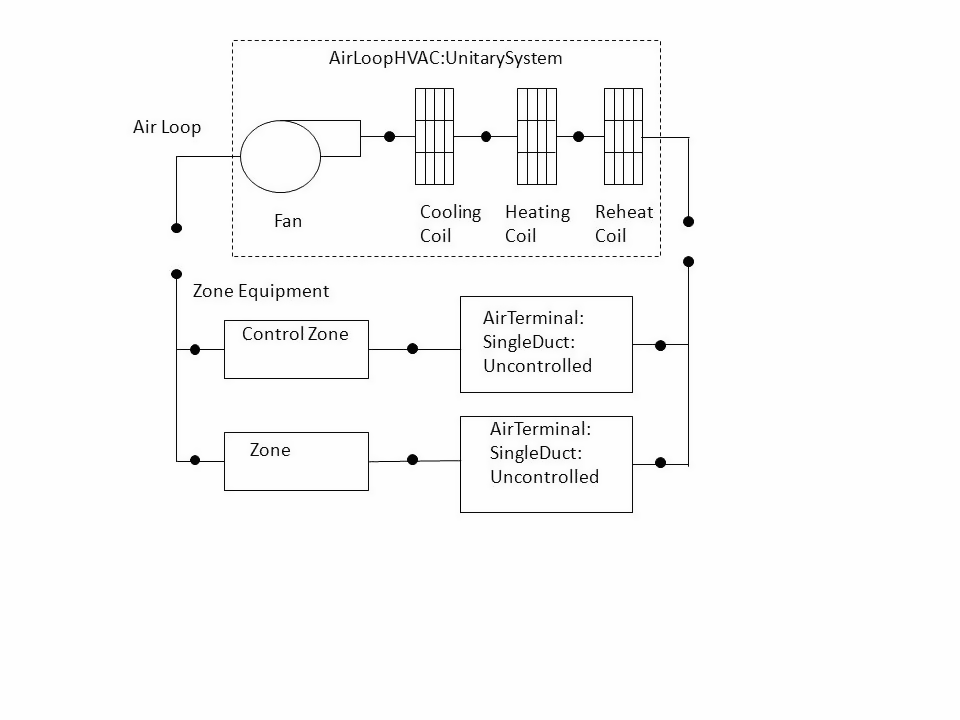
\includegraphics[width=0.9\textwidth, height=0.9\textheight, keepaspectratio=true]{media/image4930.png}
\caption{Schematic of the EnergyPlus Unitary System (Blow Through Configuration) \protect \label{fig:schematic-of-the-energyplus-unitary-system}}
\end{figure}

\subsubsection{Model Description}\label{model-description}

As described previously, the unitary system is a ``virtual'' component consisting of a fan, heating coil, cooling coil and reheat coil. The sole purpose of the unitary system model is to properly coordinate the operation of the various system components. The following sections describe the flow of information within the model, as well as the differences between cycling and continuous supply air fan operation.

\subsubsection{Controls}\label{controls}

There are three types of control types allowed to be specified in the unitary system which are setpoint based, load based or a load based control method according to ASHRAE Standard 90.1. Each control type is described in detail below.

\subsubsection{Setpoint based control:}\label{setpoint-based-control}

The unitary system calculates the current sensible load using the temperature of the inlet node and the System Node Setpoint Temp on the control node. If the control node is not the outlet node, the desired outlet node temperature is adjusted for the current temperature difference between the outlet node and the control node. Likewise, the current latent load is calculated using the humidity ratio of the inlet node and the System Node Humidity Ratio Max on the control node. The controls determine the required coil run-time fraction and dehumidification mode (if applicable) using the steps outlined below.

\paragraph{Step 1 -- Meet Sensible Load Requirement}\label{step-1-meet-sensible-load-requirement}

The controls first attempt to meet the sensible requirement. The specified coil model is called with a part-load ratio (PLR) of 1.0 to determine the full-load output of the coil. This is compared with the desired outlet node temperature and a sensible PLR is calculated. If the PLR is \textless{}1.0, a root solver iteration routine is called to determine the coil run-time fraction which results in the desired outlet node temperature. For a variable-speed DX cooling coil, if the load is smaller than the sensible capacity at the lowest speed, the coil run-time fraction is determined in the same way as a single-speed DX cooling coil. Otherwise, its speed number and speed ratio between two neighboring speeds are selected to match the load.

\paragraph{Step 2 -- Meet Latent Load Requirement (if activated)}\label{step-2-meet-latent-load-requirement-if-activated}

If dehumidification controls are active, the leaving humidity ratio resulting from operation to meet the sensible load (Step 1 above) is compared with the desired outlet node humidity ratio. If the humidity requirement is already met, then no further control action is taken. If the humidity requirement has not been met, then the coil is re-simulated depending on the type of humidity control.

\paragraph{Step 2a -- Humidity Control = MultiMode}\label{step-2a-humidity-control-multimode}

If the humidity control type is MultiMode, then the coil's enhanced dehumidification mode is activated when the coil type is Coil:Cooling:DX:TwoStageWithHumidityControlMode and Step 1 above is repeated to meet the sensible load using the coil performance resulting from the enhanced dehumidification mode. This is a semi-passive approach to dehumidification which may fall short or may exceed the dehumidification requirement.

\paragraph{Step 2b -- Humidity Control = CoolReheat}\label{step-2b-humidity-control-coolreheat}

If the humidity control type is CoolReheat, the coil is re-simulated to achieve the desired outlet node humidity ratio. This option is valid for all cooling coil types. When the coil type is Coil:Cooling:DX:TwoStageWithHumidityControlMode, only the cooling performance mode is used for this step and enhanced dehumidification mode is not activated.

\subsubsection{Load based control:}\label{load-based-control}

While the unitary system may be configured to serve multiple zones, system operation is controlled by a thermostat located in a single ``control'' zone. One of the key parameters for the unitary system component is the fraction of the total system air flow that goes through the control zone. This fraction is calculated as the ratio of the maximum air mass flow rate for the air loop's supply inlet node for the control zone (e.g., AirTerminal:SingleDuct:ConstantVolume:NoReheat, field = Maximum Air Flow Rate, converted to mass flow) to the sum of the maximum air mass flow rates for the air loop's supply inlet nodes for all zones served by this air loop. The unitary system module scales the calculated load for the control zone upward based on this fraction to determine the total load to be met by the unitary system. The module then proceeds to calculate the required part-load ratio for the system coil and the supply air fan to meet this total load. The heating or cooling capacity delivered by the unitary system is distributed to all of the zones served by this system via the terminal units that supply air to each zone. The supply air fraction that goes though the control zone is calculated as follows:

\begin{equation}
Control Zone Air Flow\,Fraction = \frac{{{{\dot m}_{TUMax\,ControlZone}}}}{{\sum\limits_{j = 1}^{NumOfZones} {{{\dot m}_{TUMax\,Zone\,j}}} }}
\end{equation}

where:

\({\dot m_{TUMax\,ControlledZone}}\) is the maximum air mass flow rate for the air loop's supply inlet node (terminal unit) for the control zone (kg/s)

\({\dot m_{TUMax\,Zone\,j}}\) is the maximum air mass flow rate for the air loop's supply inlet node for the jth zone (kg/s)

\(NumOfZones\) is the number of zones, or number of air loop supply air inlet nodes for all zones served by the air loop.

The unitary system component is able to model supply air fan operation in two modes: cycling fan -- cycling coil (i.e., AUTO fan) and continuous fan -- cycling coil (i.e., fan ON). Fan:OnOff must be used to model AUTO fan, while Fan:OnOff or Fan:ConstantVolume can be used to model fan ON. The fan operation mode is specified using a supply air fan operating mode schedule where schedule values of 0 denote cycling fan operation and schedule values other than 0 (a 1 is usually used) denote continuous fan operation. Using this schedule, the unitary system fan may be cycled with cooling or heating coil operation or operated continuously based on time of day (e.g., cycling fan operation at night and continuous fan operation during the daytime). If the fan operating mode schedule name field is left blank in the unitary system object, the unitary system assumes cycling or AUTO fan mode operation throughout the simulation.

The unitary system operates based on the user-specified (or autosized) design supply air flow rate(s). The `design' supply air mass flow rate may be different for cooling, heating, and when no cooling or heating is required and the fan operates continuously based on user-specified inputs.

\textbf{Cooling Operation}

If EnergyPlus determines that the unitary system must supply cooling to the control zone to meet the zone air temperature setpoint, then the model computes the total sensible cooling load to be met by the unitary system based on the control zone sensible cooling load and the fraction of the unitary system air flow that goes through the control zone.

\begin{equation}
UnitarySystemCoolingLoad = \frac{{ControlZoneCoolingLoad}}{{ControlZoneAirFlowFraction}}
\label{eq:UnitarySystemCoolingLoad}
\end{equation}

If the supply air fan operating mode schedule requests cycling fan operation, the model first checks for the presence of an economizer in the outside air system serving the unitary system's air loop (Ref. AirLoopHVAC:OutdoorAirSystem). If an outside air system is not present or if an air-side economizer is not used, the unitary system's compressor is used to meet the unitary system cooling load. If an air-side economizer is used and is active (i.e., economizer controls indicate that conditions are favorable to increase the outside air flow rate), the unitary system will try to meet the cooling load by operating only the supply air fan. If the fan is able to satisfy the unitary system cooling load, the compressor remains off for the entire simulation time step. If the operation of the fan alone is unable to meet the entire cooling load, then the compressor is enabled and additional calculations are performed to determine the compressor's part-load ratio.

The model then calculates the unitary system's sensible cooling energy rate delivered to the zones being served when the system runs at full-load conditions and when the cooling coil is OFF. If the supply air fan cycles with the compressor, then the sensible cooling energy rate is zero when the cooling coil is OFF. However if the fan is configured to run continuously regardless of coil operation, then the sensible cooling energy rate will probably not be zero when the cooling coil is OFF. Calculating the sensible cooling energy rate involves modeling the supply air fan (and associated fan heat), the cooling coil, and the heating and reheat coil (simply to pass the air properties and mass flow rate from its inlet node to its outlet node). For each of these cases (full load and cooling coil OFF), the sensible cooling energy rate delivered by the unitary system is calculated as follows:

\begin{equation}
Full~Cool~Output = (Mass~Flow~Rat{e_{full\;load}}){({h_{out,full~load}} - {h_{control~zone}})_{HR\min }} - {\Delta_{sen,full~load}}
\end{equation}

\begin{equation}
No~Cool~Output = (Mass~Flow~Rat{e_{coil~off}}){({h_{out,coil~off}} - {h_{control~zone}})_{HRmin }} - {\Delta_{sen,coil~off}}
\end{equation}

where:

\emph{Mass Flow Rate\(_{full~load}\)} is the air mass flow rate through unitary system at full-load conditions (kg/s)

\emph{h\(_{coil, full~load}\)} is the enthalpy of air exiting the unitary system at full-load conditions (J/kg)

\(h_{\rm{control~zone}}\) is the enthalpy of air in the control zone where the thermostat is located (J/kg)

\emph{HR\(_{min}\)} is the enthalpies evaluated at a constant humidity ratio, the minimum humidity ratio of the unitary system exiting air or the air in the control zone

\emph{Mass Flow Rate\(_{coil~off}\)} is the air mass flow rate through the unitary system with the cooling coil OFF (kg/s)

\emph{h\(_{out,coil~off}\)} is the enthalpy of air exiting the unitary system with the cooling coil OFF (J/kg)

\(\Delta_{sen,full~load}\) is the sensible load difference between the system output node and the zone inlet node at full-load conditions.

\begin{equation}
  \begin{array}{rl}
    \Delta_{sen,full~load} &= \frac{MassFlowRate_{Zone~Inlet}}{Frac} \PB{h_{Out,full~load} - h_{Zone~Inlet}}_{HRmin} \\
                           &+ \PB{MassFlowRate_{full~load} - \frac{MassFlowRate_{Zone~Inlet}}{Frac}} \PB{ h_{Out,full~load} - h_{Control~Zone}}_{HRmin}
  \end{array}
\end{equation}

where:

Frac is the control zone air fraction with respect to the system mass flow rate

\(\Delta_{sen,coil off}\) is the sensible load difference between the system output node and the zone inlet node with the heating coil OFF conditions.

\begin{equation}
  \begin{array}{rl}
    \Delta_{sen,coil~off} &= \frac{MassFlowRate_{Zone~Inlet}}{Frac} \PB{h_{Out,coil~off} - h_{Zone~Inlet}}_{HRmin} \\
                           &+ \PB{MassFlowRate_{coil~off} - \frac{MassFlowRate_{Zone~Inlet}}{Frac}} \PB{ h_{Out,coil~off} - h_{Control~Zone}}_{HRmin}
  \end{array}
\end{equation}

With the calculated sensible cooling energy rates and the total sensible cooling load to be met by the system, the part-load ratio for the unitary system is estimated.

\begin{equation}
PartLoadRatio = MAX\left( {0.0,\frac{{\left( {UnitarySystemCoolingLoad - NoCoolOutput} \right)}}{{\left( {FullCoolOutput - NoCoolOutput} \right)}}} \right)
\end{equation}

Since the part-load performance of the cooling coil is frequently non-linear, and the supply air fan heat varies based on cooling coil operation for the case of cycling fan/cycling coil (AUTO fan), the final part-load ratio for the cooling coil compressor and fan are determined through iterative calculations (successive modeling of the cooling coil and fan) until the unitary system's cooling output matches the cooling load to be met within the convergence tolerance. The convergence tolerance is fixed at 0.001 and is calculated based on the difference between the load to be met and the unitary system's cooling output divided by the load to be met.

\begin{equation}
Tolerance = 0.001 \ge \frac{{\left( {UnitarySystemCoolingLoad - {Q_{UnitarySystem}}} \right)}}{{UnitarySystemCoolingLoad}}
\end{equation}

where \({Q_{UnitarySystem}}\) is the unitary system delivered sensible capacity (W).

If the unitary system has been specified with cycling fan/cycling coil (AUTO fan), then the unitary system's operating supply air mass flow rate is multiplied by PartLoadRatio to determine the average air mass flow rate for the system simulation time step. In this case, the air conditions at nodes downstream of the cooling coil represent the full-load (steady-state) values when the coil is operating.

If the fan operates continuously (i.e., when the supply air fan operating mode schedule values are NOT equal to 0), the operating air mass flow rate through the unitary system is calculated as the average of the user-specified air flow rate when the cooling coil is ON and the user-specified air flow rate when the cooling coil is OFF (user-specified supply air volumetric flow rates converted to dry air mass flow rates).

\begin{equation}
{\dot{m}_{UnitarySystem}} = PartLoadRatio\left( {{\dot{m}_{CoolCoilON}}} \right) + \left( {1 - PartLoadRatio} \right)\left( {{\dot{m}_{CoilOFF}}} \right)
\end{equation}

where:

\(\dot m_{HeatCoilON}\) is the air mass flow rate through unitary system when the cooling coil is ON (kg/s)

\(\dot m_{CoilOFF}\) is the air mass flow rate through unitary system when no cooling or heating is needed (kg/s).

In this case, the air conditions at nodes downstream of the cooling coil are calculated as the average conditions over the simulation time step (i.e., the weighted average of full-load conditions when the coil is operating and inlet air conditions when the coil is OFF).

\textbf{Cooling Operation (multi or variable speed coils)}

After the unitary system cooling load is determined as described in Equation~\ref{eq:UnitarySystemCoolingLoad} above, the multi or variable speed cooling coil models calculations are described in this section.

The model calculates the unitary system's sensible cooling energy rate delivered to the zones being served when the system runs at full-load conditions at the highest speed and when the DX cooling coil is OFF. If the supply air fan cycles with the compressor, then the sensible cooling energy rate is zero when the cooling coil is OFF. However if the fan is scheduled to run continuously regardless of coil operation, then the sensible cooling energy rate will not be zero when the cooling coil is OFF. Calculating the sensible cooling energy rate involves modeling the supply air fan (and associated fan heat) and the multi/variable speed DX cooling coil. The multi/variable speed DX heating coil and the supplemental heating coil are also modeled, but only to pass the air properties and mass flow rate from their inlet nodes to their outlet nodes. For each of these cases (full load at highest cooling speed and DX cooling coil OFF), the sensible cooling energy rate delivered by the unitary system is calculated as follows:

\begin{equation}
  FullCoolOutpu{t_{Highest\;Speed}} = ({\dot m_{HighestSpeed}}){({h_{out,full~load}} - {h_{control~zone}})_{HRmin}} - {\Delta_{sen,HighestSpeed}}
\end{equation}

\begin{equation}
  NoCoolOutput = ({\dot m_{CoilOff}}){({h_{out,coil~off}} - {h_{control~zone}})_{HRmin}} - {\Delta_{sen,coil~off}}
\end{equation}

where:

\({\dot m_{HighestSpeed}}\) is the air mass flow rate through unitary system at the highest cooling speed (kg/s)

\(h_{out,full~load}\) is the enthalpy of air exiting the unitary system at full-load conditions {[}J/kg{]}

\(h_{control~zone}\) is the enthalpy of air leaving the control zone (where thermostat is located) (J/kg)

\(HR_{min}\) is the minimum humidity ratio of the unitary system exiting air or the air leaving the control zone (kg/kg)

\({\dot m_{CoilOff}}\) is the air mass flow rate through the unitary system with the cooling coil OFF (kg/s)

\(h_{out,coil~off}\) is the enthalpy of air exiting the unitary system with the cooling coil OFF (J/kg)

\(\Delta_{sen,HighestSpeed}\) is the sensible load difference between the system output node and the zone inlet node at full-load conditions

\(\Delta_{sen,coil~off}\) is the sensible load difference between the system output node and the zone inlet node with the cooling coil OFF conditions.

\begin{equation}
\begin{array}{rl}
{\Delta_{sen,HighestSpeed}} = & \frac{\dot{m}_{Zone~Inlet}}{Frac} {\left( {{h_{Out,full~load}} - {h_{Zone~Inlet}}} \right)_{HRmin}} \\
 & + \left( {\dot{m}_{HighestSpeed}} - \frac{\dot{m}_{Zone~Inlet}}{Frac} \right){\left( {{h_{Out,full~load}} - {h_{Control~Zone}}} \right)_{HRmin}}
\end{array}
\end{equation}

\begin{equation}
\begin{array}{rl}
{\Delta_{sen,coil~off}} = & \frac{\dot{m}_{Zone~Inlet}}{Frac} {\left( {{h_{Out,coil~off}} - {h_{Zone~Inlet}}} \right)_{HRmin}} \\
 & + \left( {\dot{m}_{coil~off}} - \frac{\dot{m}_{Zone~Inlet}}{Frac} \right) {\left( {{h_{Out,coil~off}} - {h_{Control~Zone}}} \right)_{HRmin}}
\end{array}
\end{equation}

where Frac is the control zone air fraction with respect to the system mass flow rate.

If the unitary system's sensible cooling rate at the highest speed (full load, no cycling) is insufficient to meet the entire cooling load, the controlled zone conditions will not be met. The reported cycling rate and speed ratio are 1, and the speed number is set to the highest index number. If the total sensible cooling load to be met by the system is less than the sensible cooling rate at the highest speed, then the following steps are performed.

First, calculate the sensible cooling energy rate at Speed 1:

\begin{equation}
FullCoolOutpu{t_{Speed1}} = ({\dot m_{Speed1}}){({h_{out,fullload}} - {h_{control~zone}})_{HRmin}} - {\Delta_{sen,Speed1}}
\end{equation}

where:

\emph{\({\dot m_{Speed1}}\)} is the air mass flow rate through unitary system at Speed 1 (kg/s)

\(\Delta_{sen,Speed1}\) is th sensible load difference between the system output node and the zone inlet node at full-load conditions at Speed 1.

\begin{equation}
  \begin{split}
    \Delta_{sen,Speed1} =& \frac{\dot{m}_{Zone~Inlet}}{Frac} \PB{h_{Out,full~load} - h_{Zone~Inlet}}_{HRmin} \\
                              &+ \PB{\dot{m}_{Speed1} - \frac{\dot{m}_{Zone~Inlet}}{Frac}} \PB{h_{Out,full~load} - h_{Control~Zone}}_{HRmin}
  \end{split}
\end{equation}

If the sensible cooling energy rate delivered by the unitary system at Speed 1 is greater or equal to the sensible load, the cycling ratio (part-load ratio) for the unitary system is estimated.

\begin{equation}
  \begin{array}{rl}
    CyclingRatio &= \frac{ \left| \PB{CoolingCoilSensibleLoad} \right| } {FullCoolingCoilCapacity} \\ 
                 &= \max \PB{0.0,\frac{UnitarySystemCoolingLoad - AddedFanHeat}{FullCoolOutput_{Speed1} - AddedFanHeat_{Speed1}}}
  \end{array}
\end{equation}

where:

\emph{AddedFanHeat} is the generated supply air fan heat, which is a function of part load ratio and as internal component cooling load (W)

\emph{AddedFanHeat\(_{Speed1}\)} is the generated supply air fan heat at Speed 1 for a part load ratio = 1 (W).

Since the part-load performance of the DX cooling coil is frequently non-linear,and the supply air fan heat varies based on cooling coil operation for the case of cycling fan/cycling coil (AUTO fan), the final part-load ratio for the cooling coil compressor and fan are determined through iterative calculations (successive modeling of the cooling coil and fan) until the unitary system's cooling output matches the cooling load to be met within the convergence tolerance. The convergence tolerance is fixed at 0.001 and is calculated based on the difference between the load to be met and the unitary system's cooling output divided by the load to be met.

\begin{equation}
Tolerance = 0.001 \ge \frac{{\left( {UnitarySystemOutpu{t_{cycling}} - {Q_{UnitarySystem}}} \right)}}{{UnitarySystemCoolingLoad}}
\end{equation}

where the UnitarySystemOutput\(_{Cycling}\) is the unitary system delivered sensible capacity for Speed 1 operating at a specific cycling ratio (W).

\begin{equation}
UnitarySystemOutpu{t_{cycling}} = {\dot{m}_{UnitarySystem}}{\left( {{h_{out}} - {h_{ControlZone}}} \right)_{HR\min }} - {\Delta_{cycling}}
\end{equation}

where:

\({\dot m{_{UnitarySystem}}}\) is the average air mass flow rate defined in the next section (kg/s)

\emph{h\(_{out}\)} is the enthalpy of air exiting the unitary system at part load conditions (J/kg)

Δ\(_{cycling}\) is the average sensible load difference between the system output node and the zone inlet node.

\begin{equation}
{\Delta_{cycling}} = \frac{\dot{m}_{ZoneInlet}}{frac} \left( {{h_{ZoneInlet}} - {h_{ControlZone}}} \right) + \left( {\dot{m}_{UnitarySystem}} - \frac{\dot{m}_{ZoneInlet}}{frac} \right) \left( {{h_{Out}} - {h_{ControlZone}}} \right)
\end{equation}

where \({\dot m{_{ZoneInlet}}}\) is the air mass flow rate in the supply inlet node in the controlled zone (kg/s).

For this case where speed 1 operation was able to meet the required cooling load, the speed ratio is set to zero and speed number is equal to 1.

If the unitary system's cooling output at full load for Speed 1 is insufficient to meet the entire cooling load, the Cycling ratio is set equal to 1.0 (compressor and fan are not cycling). Then the cooling speed is increased and the delivered sensible capacity is calculated. If the full load sensible capacity at Speed n is greater than or equal to the sensible load, the speed ratio for the unitary system is estimated:

\begin{equation}
SpeedRatio = \frac{{ABS\left( {UnitarySystemCoolingLoad - AddedFanHeat - FullCoolOutpu{t_{Speedn - 1}}} \right)}}{{ABS\left( {FullCoolOutpu{t_{Speedn}} - FullCoolOutpu{t_{Speedn - 1}}} \right)}}
\end{equation}

Although a linear relationship is assumed by applying the speed ratio to obtain the effective capacity and mass flow rate between speed n and n-1, the outlet air node conditions are dependent on the combined outputs and may not be linear. In addition, the supply air fan heat varies with the speed ratio due to different supply mass flow rates between speed n and n-1 . Therefore, the final speed ratio for the cooling coil compressor and fan are determined through iterative calculations (successive modeling of the cooling coil and fan) until the unitary system's cooling output matches the cooling load to be met within the convergence tolerance. The convergence tolerance is fixed at 0.001 and is calculated based on the difference between the load to be met and the unitary system's cooling output divided by the load to be met.

\begin{equation}
Tolerance = 0.001 \ge \frac{{\left( {UnitarySystemCoolingLoad - UnitarySystemOutpu{t_{SpeedRatio}}} \right)}}{{UnitarySystemCoolingLoad}}
\end{equation}

where \emph{UnitarySystemOutput\(_{Speedn}\)} is the unitary system delivered sensible capacity between two consecutive speeds at a specific speed ratio (W).

\begin{equation}
  \begin{array}{rl}
    UnitarySystemOutput_{SpeedRatio} =& (SpeedRatio)FullCoolOutput_{Speedn} \\
                                     &+ (1 - SpeedRatio)FullCoolOutput_{Speedn - 1} \\
                                     &- AddedFanHeat_{SpeedRatio}
  \end{array}
\end{equation}

where \emph{AddedFanHeat\(_{SpeedRatio}\)} is the generated supply air fan heat at a specific speed ratio (W).

In this case, the reported cycling ratio is 1 and speed number is equal to n.

\paragraph{Air Mass Flow Rate Calculation}\label{air-mass-flow-rate-calculation}

\emph{Speed 1 operation}

If the unitary system has been specified with cycling fan/cycling coil (AUTO fan), then the unitary system's operating supply air mass flow rate is determined by the cycling ratio (PartLoadRatio) for Speed 1. The supply air mass flow rate is multiplied by the cycling ratio to determine the average air mass flow rate for the system simulation time step. The air conditions at nodes downstream of the cooling coils represent the full-load (steady-state) values when the coil is operating.

\begin{equation}
\dot{m}_{UnitarySystem} = \left( {CyclingRatio} \right)\dot{m}_{Speed1}
\end{equation}

If the fan operates continuously (i.e., when the supply air fan operating mode schedule values are NOT equal to 0), the operating air mass flow rate through the unitary system is calculated as the average of the user-specified air flow rate when the unitary system cooling coil is ON at Speed 1 and the user-specified air flow rate when the unitary system cooling coil is OFF (user-specified supply air volumetric flow rates converted to dry air mass flow rates).

\begin{equation}
{\dot{m}_{UnitarySystem}} = \left( {CyclingRatio} \right){\dot{m}_{Speed1}} + \left( {1 - CyclingRatio} \right){\dot{m}_{CoilOff}}
\end{equation}

where:

\({\dot m_{UnitarySystem}}\) is the average air mass flow rate through unitary system (kg/s)

\({\dot m_{Speed1}}\) is the air mass flow rate through unitary system when cooling coil is ON at Speed 1 (kg/s)

\({\dot m_{CoilOff}}\) is the air mass flow rate through unitary system when no heating or cooling is needed (kg/s).

In this case, the air conditions at nodes downstream of the cooling coils are calculated as the average conditions over the simulation time step (i.e., the weighted average of full-load conditions when the coil is operating and inlet air conditions when the coil is OFF).

\paragraph{Higher Speed Operation}\label{higher-speed-operation}

When the unitary system operates at higher speeds to meet the required cooling load, the supply air mass flow rate is linearly interpolated between two consecutive speeds:

\begin{equation}
{\dot{m}_{UnitarySystem}} = \left( {SpeedRatio} \right){\dot{m}_{Speedn}} + \left( {1 - SpeedRatio} \right){\dot{m}_{Speedn - 1}}
\end{equation}

where:

\(\dot{m}_{UnitarySystem}\) is the average air mass flow rate through the unitary system for the time step (kg/s)

\(\dot m_{Speedn}\) is the air mass flow rate through unitary system when cooling coil is ON at Speed n (kg/s)

\(\dot m_{Speedn - 1}\) is the air mass flow rate through unitary system when cooling coil is ON at Speed n-1 (kg/s).

For this case of higher speed operation, the air conditions at nodes downstream of the cooling coils are determined by the delivered cooling capacity and supply air mass flow rates between two consecutive speeds.

Although the above sections present the capacity and air mass flow rate calculation separately, they are dependent and change every iteration until convergence is reached for the time step being simulated.

\textbf{Heating Operation}

Calculations for heating operation are similar to those for cooling operation in most respects. However, due to the inclusion of a supplemental heating coil, additional calculations are necessary to properly meet the total heating load for the zones being served.

If EnergyPlus determines that the unitary system must supply heating to the control zone to meet the zone air temperature setpoint, then the unitary system model computes the total sensible heating load to be delivered to the zones being served based on the control zone sensible heating load and the control zone airflow fraction.

\begin{equation}
UnitarySystemHeatingLoad = \frac{{ControlZoneHeatingLoad}}{{ControlZoneAirFlowFraction}}
\label{eq:UnitarySystemHeatingLoad}
\end{equation}

The model then calculates the unitary system's sensible heating energy rate delivered to the zones being served when the system runs at full-load conditions and when the heating coil is OFF (without supplemental heater operation in either case). If the supply air fan cycles with the compressor, then the sensible heating energy rate is zero when the compressor is OFF. However if the fan is scheduled to run continuously regardless of coil operation, then the sensible heating energy rate will not be zero when the compressor is OFF. Calculating the sensible heating energy rate involves modeling the supply air fan (and associated fan heat), the~ cooling coil (simply to pass the air properties and mass flow rate from its inlet node to its outlet node), the~ heating coil, and the supplemental heating coil (simply to pass the air properties and mass flow rate from its inlet node to its outlet node). For each of these cases (full load and~ heating coil OFF, without supplemental heater operation in either case), the sensible heating energy rate delivered by the unitary system is calculated as follows:

\begin{equation}
Full~Heat~Output = (Mass~Flow~Rat{e_{full~load}}){({h_{out,full~load}} - {h_{control~zone}})_{HRmin}} - {\Delta_{sen,full~load}}
\end{equation}

\begin{equation}
No~Heat~Output = (Mass~Flow~Rat{e_{coil~off}}){({h_{out,coil~off}} - {h_{control~zone}})_{HRmin}} - {\Delta_{sen,coil~off}}
\end{equation}

where:

\emph{Mass Flow Rate\(_{full~load}\)} is the air mass flow rate through unitary system at full-load conditions (kg/s)

\emph{h\(_{out, full~load}\)} is the enthalpy of air exiting the unitary system at full-load conditions (J/kg)

\emph{h\(_{control~zone}\)} is the enthalpy of air leaving the control zone (where thermostat is located) (J/kg)

\emph{HR\(_{min}\)} are the enthalpies evaluated at a constant humidity ratio, the minimum humidity ratio of the unitary system exiting air or the air leaving the control zone

\emph{Mass Flow Rate\(_{coil~off}\)} is the air mass flow rate through the unitary system with the heating coil OFF (kg/s)

\emph{h\(_{out,coil~off}\)} is the enthalpy of air exiting the unitary system with the heating coil OFF (J/kg)

\(\Delta_{sen,full~load}\) is the sensible load difference between the system output node and the zone inlet node at full-load conditions.

\begin{equation}
  \begin{split}
    \Delta_{sen,full~load} =& \frac{\dot{m}_{Zone~Inlet}}{Frac} \PB{h_{Out,full~load} - h_{Zone~Inlet}}_{HRmin} \\
                              &+ \PB{\dot{m}_{full~load} - \frac{\dot{m}_{Zone~Inlet}}{Frac}} \PB{h_{Out,full~load} - h_{Control~Zone}}_{HRmin}
  \end{split}
\end{equation}

where:

Frac is the control zone air fraction with respect to the system mass flow rate

\(\Delta_{sen,coil~off}\) is the sensible load difference between the system output node and the zone inlet node with the heating coil OFF conditions.

\begin{equation}
  \begin{split}
    \Delta_{sen,coil~off} =& \frac{\dot{m}_{Zone~Inlet}}{Frac} \PB{h_{Out,coil~off} - h_{Zone~Inlet}}_{HRmin} \\
                              &+ \PB{\dot{m}_{coil~off} - \frac{\dot{m}_{Zone~Inlet}}{Frac}} \PB{h_{Out,coil~off} - h_{Control~Zone}}_{HRmin}
  \end{split}
\end{equation}

With the calculated sensible heating energy rates and the total sensible heating load to be met by the system, the part-load ratio for the unitary system is estimated.

\begin{equation}
PartLoadRatio = MAX\left( {0.0,\frac{{\left( {UnitarySystemHeatingLoad - NoHeatOutput} \right)}}{{\left( {FullHeatOutput - NoHeatOutput} \right)}}} \right)
\end{equation}

Since the part-load performance of the~ heating coil is frequently non-linear, and the supply air fan heat varies based on heating coil operation for the case of cycling fan/cycling coil (AUTO fan), the final part-load ratio for the heating coil compressor and fan are determined through iterative calculations (successive modeling of the heating coil and fan) until the unitary system's heating output matches the heating load to be met within the convergence tolerance. The convergence tolerance is fixed at 0.001 and is calculated based on the difference between the load to be met and the unitary system's heating output divided by the load to be met.

\begin{equation}
Tolerance = 0.001 \ge \frac{{\left( {UnitarySystemHeatingLoad - {Q_{UnitarySystem}}} \right)}}{{UnitarySystemHeatingLoad}}
\end{equation}

where \({Q_{UnitarySystem}}\) is the unitary system delivered sensible capacity (W).

If the unitary system's~ heating coil output at full load is insufficient to meet the entire heating load, PartLoadRatio is set equal to 1.0 (compressor and fan are not cycling) and the remaining heating load is passed to the supplemental heating coil. If the unitary system model determines that the outdoor air temperature is below the minimum outdoor air temperature for compressor operation, the compressor is turned off and the entire heating load is passed to the supplemental gas or electric heating coil. The unitary system exiting air conditions and energy consumption are calculated and reported by the individual component models (fan,~ heating coil, and supplemental gas or electric heating coil).

If the unitary system has been specified with cycling fan/cycling coil (AUTO fan), then the unitary system's operating supply air mass flow rate is multiplied by PartLoadRatio to determine the average air mass flow rate for the system simulation time step. The air conditions at nodes downstream of the heating coils represent the full-load (steady-state) values when the coils are operating. If the fan operates continuously (i.e., when the supply air fan operating mode schedule values are NOT equal to 0), the operating air mass flow rate through the unitary system is calculated as the average of the user-specified air flow rate when the unitary system heating coil is ON and the user-specified air flow rate when the unitary system heating coil is OFF (user-specified supply air volumetric flow rates converted to dry air mass flow rates).

\begin{equation}
\dot{m}_{UnitarySystem} = PartLoadRatio\left( \dot{m}_{HeatCoilON} \right) + \left( 1 - PartLoadRatio \right)\left( \dot{m}_{CoilOFF} \right)
\end{equation}

where:

\(\dot m_{HeatCoilON}\) is the air mass flow rate through unitary system when the heating coil is ON (kg/s)

\(\dot m_{CoilOFF}\) is the air mass flow rate through unitary system when no heating or cooling is needed (kg/s).

In this case, the air conditions at nodes downstream of the heating coils are calculated as the average conditions over the simulation time step (i.e., the weighted average of full-load conditions when the coils are operating and inlet air conditions when the coils are OFF).

\subsubsection{Heating Operation (multi or variable speed coils )}\label{heating-operation-multi-or-variable-speed-coils}

After the unitary system heating load is determined as described in Equation~\ref{eq:UnitarySystemHeatingLoad} above, the multi or variable speed heating coil models calculation are described in this section.

The model calculates the unitary system's sensible heating energy rate delivered to the zones being served when the system runs at full-load conditions at the highest speed and when the DX heating coil is OFF (without supplemental heater operation in either case). If the supply air fan cycles with the compressor, then the sensible heating energy rate is zero when the compressor is OFF. However if the fan is scheduled to run continuously regardless of coil operation, then the sensible heating energy rate will not be zero when the compressor is OFF. Calculating the sensible heating energy rate involves modeling the supply air fan (and associated fan heat), the DX cooling coil (simply to pass the air properties and mass flow rate from its inlet node to its outlet node), the DX heating coil, and the supplemental heating coil (simply to pass the air properties and mass flow rate from its inlet node to its outlet node). For each of these cases (full load and DX heating coil OFF, without supplemental heater operation in either case), the sensible heating energy rate delivered by the unitary system is calculated as follows:

\begin{equation}
FullHeatOutpu{t_{HighestSpeed}} = ({\dot m_{HighestSpeed}}){({h_{out,full~load}} - {h_{control~zone}})_{HRmin}} - {\Delta_{sen,HighestSpeed}}
\end{equation}

\begin{equation}
NoHeatOutput = ({\dot m_{CoilOff}}){({h_{out,coil~off}} - {h_{control~zone}})_{HRmin}} - {\Delta_{sen,coil~off}}
\end{equation}

where:

\emph{\({\dot m_{HighestSpeed}}\)} is the air mass flow rate through unitary system at the highest heating speed (kg/s)

\emph{h\(_{out, full~load}\)} is the enthalpy of air exiting the unitary system at full-load conditions (J/kg)

\emph{h\(_{control~zone}\)} is the enthalpy of air leaving the control zone (where thermostat is located) (J/kg)

\emph{HR\(_{min}\)} are the enthalpies evaluated at a constant humidity ratio, the minimum humidity ratio of the unitary system exiting air or the air leaving the control zone

\({\dot m_{CoilOff}}\) is the air mass flow rate through the unitary system with the heating coil OFF (kg/s)

\emph{h\(_{out,coil~off}\)} is the enthalpy of air exiting the unitary system with the heating coil OFF (J/kg)

\(\Delta_{sen,full~load}\) is the sensible load difference between the system output node and the zone inlet node at full-load conditions.

\begin{equation}
  \begin{split}
    \Delta_{sen,HighestSpeed} =& \frac{\dot{m}_{Zone~Inlet}}{Frac} \PB{h_{Out,full~load} - h_{Zone~Inlet}}_{HRmin} \\
                              &+ \PB{\dot{m}_{HighestSpeed} - \frac{\dot{m}_{Zone~Inlet}}{Frac}} \PB{h_{Out,coil~off} - h_{Control~Zone}}_{HRmin}
  \end{split}
\end{equation}

where:

Frac is the control zone air fraction with respect to the system mass flow rate

\(\Delta_{sen,coil off}\) is the sensible load difference between the system output node and the zone inlet node with the heating coil OFF conditions.

\begin{equation}
  \begin{split}
    \Delta_{sen,coil~off} =& \frac{\dot{m}_{Zone~Inlet}}{Frac} \PB{h_{Out,coil~off} - h_{Zone~Inlet}}_{HRmin} \\
                              &+ \PB{\dot{m}_{coil~off} - \frac{\dot{m}_{Zone~Inlet}}{Frac}} \PB{h_{Out,coil~off} - h_{Control~Zone}}_{HRmin}
  \end{split}
\end{equation}

If the unitary system's DX heating coil output full load at the highest speed is insufficient to meet the entire heating load, the remaining heating load is passed to the supplemental heating coil. If the unitary system model determines that the outdoor air temperature is below the minimum outdoor air temperature for compressor operation (specified by the user), the compressor is turned off and the entire heating load is passed to the supplemental gas or electric heating coil. The unitary system exiting air conditions and energy consumption are calculated and reported by the individual component models (fan, DX heating coil, and supplemental gas or electric heating coil).

If the total heating load to be met by the system is less than the sensible heating rate at the highest speed, then the following steps are performed.

First, calculate the sensible heating energy rate at Speed 1:

\begin{equation}
FullHeatOutpu{t_{Speed1}} = ({\dot m_{Speed1}}){({h_{out,full~load}} - {h_{control~zone}})_{HRmin}} - {\Delta_{sen,Speed1}}
\end{equation}

where:

\({\dot m_{Speed1}}\) is the air mass flow rate through unitary system at Speed 1 (kg/s)

\(\Delta_{sen,Speed1}\) is the sensible load difference between the system output node and the zone inlet node at full-load conditions at Speed 1.

\begin{equation}
  \begin{split}
    \Delta_{sen,Speed1} =& \frac{\dot{m}_{Zone~Inlet}}{Frac} \PB{h_{Out,full~load} - h_{ZoneInlet}}_{HRmin} \\
                              &+ \PB{\dot{m}_{Speed1} - \frac{\dot{m}_{Zone~Inlet}}{Frac}} \PB{h_{Out,coil~off} - h_{Control~Zone}}_{HRmin}
  \end{split}
\end{equation}

Second, if the sensible heating energy rate delivered by the unitary system at Speed 1 is greater or equal to the sensible load, the cycling ratio (part-load ratio) for the unitary system is estimated.

\begin{equation}
  \begin{array}{rl}
    CyclingRatio &= \frac{\left|\PB{HeatingCoilSensibleLoad}\right|}{FullHeatingCoilCapacity} \\
                 &= \max \PB{0.0,\frac{UnitarySystemHeatingLoad - AddedFanHeat}{FullHeatOutput_{Speed1} - AddedFanHeat_{Speed1}}}
  \end{array}
\end{equation}

where:

\emph{AddedFanHeat} is the generated supply air fan heat, which is a function of part load ratio and as internal component heating load (W)

\emph{AddedFanHeat\(_{Speed1}\)} is the generated supply air fan heat at Speed 1 (part load ratio = 1) (W).

Since the part-load performance of the DX heating coil is frequently non-linear, and the supply air fan heat varies based on heating coil operation for the case of cycling fan/cycling coil (AUTO fan), the final part-load ratio for the heating coil compressor and fan are determined through iterative calculations (successive modeling of the heating coil and fan) until the unitary system's heating output matches the heating load to be met within the convergence tolerance. The convergence tolerance is fixed at 0.001 and is calculated based on the difference between the load to be met and the unitary system's heating output divided by the load to be met.

\begin{equation}
Tolerance = 0.001 \ge \frac{{\left( {UnitarySystemHeatingLoad - UnitarySystemOutpu{t_{cycling}}} \right)}}{{UnitarySystemHeatingLoad}}
\end{equation}

where \emph{UnitarySystemOutput\(_{cycling}\)} is the unitary system delivered sensible capacity for Speed 1 operating at a specific cycling ratio (W).

\begin{equation}
UnitarySystemOutput_{cycling} = \dot{m}_{UnitarySystem} \left( h_{out} - h_{Control~Zone} \right)_{HRmin} - \Delta_{cycling}
\end{equation}

where

\(\dot{m}_{UnitarySystem}\) is the average air mass flow rate defined in the next section (kg/s)

\(h_{out}\) is the enthalpy of air exiting the unitary system at part load conditions (J/kg)

\(\Delta_{cycling}\) is the average sensible load difference between the system output node and the zone inlet node.

\begin{equation}
\Delta_{cycling} = \frac{\dot{m}_{ZoneInlet}}{frac} \left( h_{ZoneInlet} - h_{ControlZone} \right) + \left( \dot{m}_{UnitarySystem} - \frac{\dot{m}_{ZoneInlet}}{frac} \right) \left( h_{Out} - h_{ControlZone} \right)
\end{equation}

where \({\dot m_{Zone~Inlet}}\) is the air mass flow rate in the supply inlet node in the controlled zone (kg/s).

For this case where Speed 1 operation was able to meet the required heating load, the speed ratio is set to zero and speed number is equal to 1.

Third, if the unitary system's heating output at full load for Speed 1 is insufficient to meet the entire heating load, the Cycling ratio (PartLoadRatio) is set equal to 1.0 (compressor and fan are not cycling). Then the heating speed is increased and the delivered sensible capacity is calculated. If the full load sensible capacity at Speed n is greater than or equal to the sensible load, the speed ratio for the unitary system is estimated:

\begin{equation}
SpeedRatio = \frac{{ABS\left( {UnitarySystemHeatingLoad - AddedFanHeat - FullHeatOutpu{t_{Speedn - 1}}} \right)}}{{ABS\left( {FullHeatOutpu{t_{Speedn}} - FullHeatOutpu{t_{Speedn - 1}}} \right)}}
\end{equation}

Although a linear relationship is assumed by applying the speed ratio to obtain the effective capacity and air mass flow rate between speed n and n-1, the outlet node conditions are dependent on the combined outputs and may not be linear. In addition, the supply air fan heat varies based on heating coil operation for the case of cycling fan/cycling coil (AUTO fan). Therefore, the final speed ratio for the heating coil compressor and fan are determined through iterative calculations (successive modeling of the heating coil and fan) until the unitary system's heating output matches the heating load to be met within the convergence tolerance. The convergence tolerance is fixed at 0.001 and is calculated based on the difference between the load to be met and the unitary system's heating output divided by the load to be met.

\begin{equation}
Tolerance = 0.001 \ge \frac{{\left( {UnitarySystemHeatingLoad - UnitarySystemOutpu{t_{SpeedRatio}}} \right)}}{{UnitarySystemHeatingLoad}}
\end{equation}

where \emph{UnitarySystemOutput\(_{SpeedRatio}\)} is the unitary system delivered sensible capacity between two consecutive speeds at a specific ratio (W).

\begin{equation}
  \begin{array}{rl}
    UnitarySystemOutput_{SpeedRatio} &= \PB{SpeedRatio} FullHeatOutput_{Speedn} \\
                                     &+ \PB{1 - SpeedRatio} FullHeatOutput_{Speedn-1} \\ 
                                     &- AddedFanHeat_{SpeedRatio}
  \end{array}
\end{equation}

where \emph{AddedFanHeat\(_{SpeedRatio}\)} is the generated supply air fan heat at a specific speed ratio (W).

In this case, the reported cycling ratio is 1 and speed number is equal to n.

\paragraph{Air Mass Flow Rate Calculation}\label{air-mass-flow-rate-calculation-1}

The air mass flow rate calculations during heating operation are the same as those described above for cooling operation for multi/variable speed.

\subsubsection{Single Zone VAV load based control:}\label{ashrae-901-load-based-control}

The unitary system can also be used to simulate a system capable of maintaining a low fan speed through a range of low to moderate loads. This control scheme is similar to single zone variable-air-volume (VAV) control where the fan speed is maintained at a minimum level and the coil is modulated to a point where the system outlet air temperature reaches a user specified limit. As the outlet air temperature limit is reached and loads increase, the fan speed increases to maintain thermostat control. When the fan speed reaches the maximum flow limit, the system outlet air temperature may exceed the user specified limit, if the coil is capable of providing more capacity, to meet increased load. This model is applicable to AirloopHVAC and ZoneHVAC equipment and is active only for constant fan operating mode. Cycling fan operating may be used, however, during time of cycling fan operating mode, the model reverts to control specified above for Load Based control. Additionally, only specific coil types are allowed for the Single Zone VAV load based control method. 

Allowed coil types are:

\textbf{Cooling coils:}
\begin{itemize}
\item Coil:Cooling:Water
\item Coil:Cooling:WaterDetailed
\item Coil:Cooling:DX:SingleSpeed
\end{itemize}

\textbf{Heating coils:}
\begin{itemize}
\item Coil:Heating:Water
\item Coil:Heating:Fuel
\item Coil:Heating:Electric
\item Coil:Heating:DX:SingleSpeed
\end{itemize}

Other coil types may be used when selecting the Single Zone VAV control method, however, these coils will not be modeled using the Single Zone VAV load based control method and instead will be modeled using the Load Based control method described in a previous section.

The example below shows two implementations of the Single Zone VAV model using the AirloopHVAC:UnitarySystem object as both air loop equipment serving multiple zones and as zone equipment serving a single zone. Chilled and hot water coils are used with autosized limits on supply air temperature. The supply air temperature limits are intended to reflect the model requirement to allow low speed fan operation at zone loads less than or equal to 50\% of the design load. The zone cooling and heating loads identified in the figure are actual simulation data taken from the zone sizing information representative of the control zones used for each system. Outdoor air loads were eliminated for this example (i.e., Outdoor Air = 0).

\begin{figure}[hbtp]
\centering
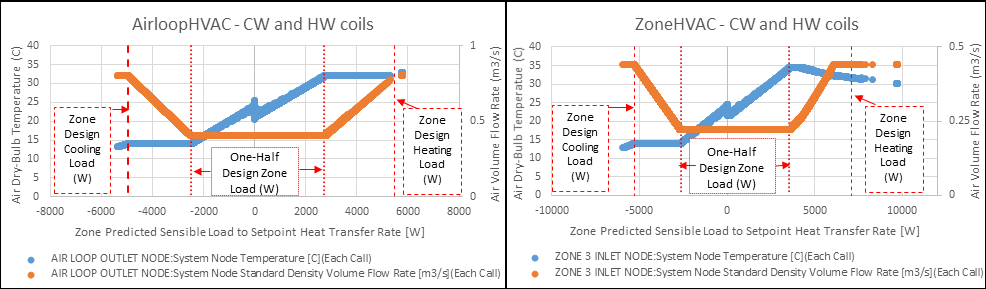
\includegraphics[width=0.9\textwidth, height=0.9\textheight, keepaspectratio=true]{media/UnitarySystem_SZVAV_watercoils.png}
\caption{Example of the EnergyPlus Unitary System Single Zone VAV Model \protect \label{fig:example-of-the-energyplus-unitary-system-single-zone-vav-model}}
\end{figure}

Supply air temperature limits are autosizable and calculated with respect to the zone temperatures at the design cooling and heating peak load conditions. Once the temperature limits are reached and the zone load continues to increase, the fan speed is increased while limiting the maximum outlet air temperature up to the maximum fan speed. At this point, the maximum temperature limits are ignored and the coils are allowed to provide excess temperatures when needed to meet increasing loads. When a supplemental heating coil is used, this coil should be active only when maximum fan speed is reached and will supplement any additional heating required to meet the zone load. The supplemental heating coil also has no maximum temperature limit while attempting to meet high heating loads.

\subsubsection{High Humidity Control}\label{high-humidity-control}

The specific configuration of the unitary system with supplemental heating coil is shown above (see Figure~\ref{fig:schematic-of-the-energyplus-unitary-system}). This figure shows the fan placement when a blow through fan is specified. If a draw through fan is specified, the fan is located between the heating coil and the supplemental heating coil. The system is controlled to keep the high relative humidity in the control zone from exceeding the setpoint specified in the object ZoneControl:Humidistat. This option is available when the supply air fan operates continuously (i.e., the supply air fan operating mode schedule values are never equal to 0) or the supply air fan cycles with the compressor. In addition, when high humidity control is specified and the compressor operates, the unitary system operates at the cooling air flow rate when a zone heating load is present as determined by the zone thermostat. High humidity control is specified as either None, MultiMode, or CoolReheat in the Dehumidification Control Type input field. MultiMode is specified when a heat exchanger is used to improve the dehumidification performance of the cooling coil. The heat exchanger will be activated when the sensible part-load ratio is insufficient to meet the zone latent load. CoolReheat is specified when a cooling coil is used to over-cool the supply air stream in order to meet the zone latent load. In this case, a supplemental heating coil will ensure the zone temperature does not fall below the zone heating temperature set point. When a heat exchanger is used in conjunction with a cooling coil and CoolReheat is specified as the Dehumidification Control Type, the heat exchanger is ``locked on'' to meet either the sensible or latent cooling load. If the dehumidification control type is selected as None and a heat exchanger assisted cooling coil is used, the heat exchanger is ``locked on'' and the air conditioner runs only to meet the sensible cooling load. A supplemental heating coil is required for all dehumidification control types.

The model first calculates the \emph{PartLoadRatio} required to meet the sensible cooling load.~ The unitary system's sensible cooling load is determined from the control zone sensible cooling load to the cooling setpoint and the control zone air flow fraction to maintain the dry-bulb temperature setpoint in the control zone.:

\begin{equation}
UnitarySystemCoolingLoad = \frac{{ControlZoneCoolingLoad}}{{ControlZoneAirFlowFraction}}
\end{equation}

The unitary system's sensible cooling load to be met and the full load cooling output are used to calculate the sensible the part-load ratio iteratively based on user specified convergence criterion.

\begin{equation}
PartLoadRatio = MAX\left( {0.0,\frac{{\left( {UnitarySystemCoolingLoad - NoCoolOutput} \right)}}{{\left( {FullCoolOutput - NoCoolOutput} \right)}}} \right)
\end{equation}

When the unitary system's sensible cooling capacity meets the system sensible cooling load at a given sensible part load ratio, then the Unitary system meets the controlled zone cooling setpoint temperature. If a moisture (latent) load exists because the control zone humidity has exceeded the setpoint, the total moisture load to be met by the unitary systems (UnitarySystemMoistureLoad) is calculated based on the control zone moisture load and the control zone air flow fraction.

\begin{equation}
UnitarySystemMoistureLoad = \frac{{ControlZoneMoistureLoad}}{{ControlZoneAirFlowFraction}}
\end{equation}

Then the \emph{LatentPartLoadRatio} required to meet the high humidity setpoint is calculated as follows:

\begin{equation}
  LatentPartLoadRatio = MIN\left( {PL{R_{Min}},\frac{{\left( {UnitarySystemMoistureLoad - NoLatentOutput} \right)}}{{\left( {FullLatentOutput - NoLatentOutput} \right)}}} \right)
\end{equation}

The model uses the greater of the two part-load ratios, \emph{PartLoadRatio} or \emph{LatentPartLoadRatio}, to determine the operating part-load ratio of the Unitary system's DX cooling coil.

\begin{equation}
LatentPartLoadRatio = MAX\left( {PartLoadRatio,LatentPartLoadRatio} \right)
\end{equation}

As previously described, iterations are performed to converge on the solution within the convergence tolerance.

where:

\(ControlZoneCoolingLoad\) is the control zone sensible cooling load to the cooling setpoint (W)

\(ControlZoneMoistureLoad\) is the control zone moisture load to the dehumidifying relative humidity setpoint (W)

\(ControlZoneAirFlowFraction\) is the supply air fraction that goes though the control zone

\(FullLatentOutput\) is the unitary system latent cooling energy rate at full-load conditions (W)

\(NoLatentOutput\) is the unitary system latent cooling energy rate with cooling coil OFF (W)

\(PartLoadRatio\) is the unitary system part-load-ratio required to meet system sensible load

\(LatentPartLoadRatio\) is the unitary system part-load-ratio required to meet system moisture load

\(PL{R_{Min}}\) is the minimum part-load ratio, which is usually 0.0. For the case when the latent capacity degradation model is used (Ref: DX Cooling Coil Model), this value is the minimum part-load ratio at which the cooling coil will dehumidify the air.

When the predicted zone air temperature is above the heating setpoint and if there is a dehumidification load, the supplemental heating coil load is required to offset the excess cooling as shown in Figure~\ref{fig:supplemental-heating-coil-load-when-predicted}. If the model determines that the LatentPartLoadRatio is to be used as the operating part-load ratio of the unitary system's cooling coil, the supplemental heating coil is used to offset the excess sensible capacity provided by the unitary system cooling coil. The model first checks the sensible load that exists for the current simulation time step (predicted zone temperature with no HVAC operation compared to the thermostat setpoint temperatures). If a sensible cooling load or no sensible cooling or heating load exists, the model calculates the difference between the sensible heating load required to reach or maintain the heating dry-bulb temperature setpoint and the actual sensible cooling energy rate delivered by the unit (with LatentPartLoadRatio). In this case, the supplemental heating coil is used to offset the excess sensible cooling energy provided by the cooling coil (if any) that could have caused an overshoot of the heating dry-bulb temperature setpoint. Note that when a humidistat is used and high humidity control is required, the zone dry-bulb temperature will typically move toward the heating temperature setpoint when a high moisture (latent) load exists.

\begin{figure}[hbtp] % fig 219
\centering
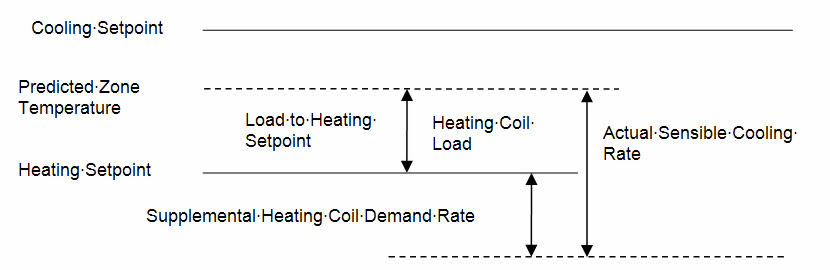
\includegraphics[width=0.9\textwidth, height=0.9\textheight, keepaspectratio=true]{media/image5015.png}
\caption{Supplemental heating coil load when predicted zone air temperature is above the heating Setpoint \protect \label{fig:supplemental-heating-coil-load-when-predicted}}
\end{figure}

If a heating load exists (Figure~\ref{fig:supplemental-heating-coil-load-when-predicted-001}), the supplemental heating coil is used to meet the heating coil load and at the same time offset the entire sensible cooling energy rate of the cooling coil (to meet the humidistat setpoint). Note that when a heating load exists and high humidity control is required, the unitary system operates at the user-specified cooling air flow rate for the entire simulation time step. As with the fan, and cooling coil, report variables associated with supplemental heating coil performance (e.g., heating coil energy, heating coil rate, heating coil gas or electric energy, heating coil runtime fraction, etc.) are managed in the supplemental (heating) coil object.

\begin{figure}[hbtp] % fig 220
\centering
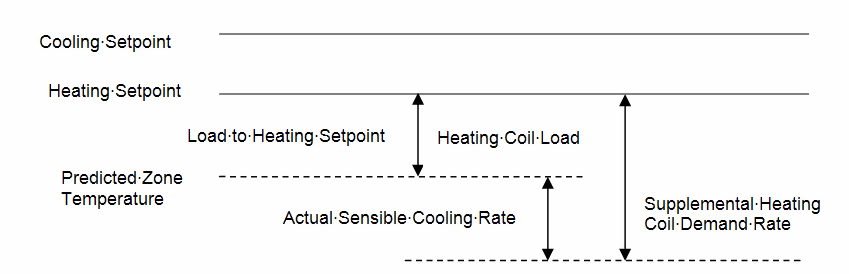
\includegraphics[width=0.9\textwidth, height=0.9\textheight, keepaspectratio=true]{media/image5016.png}
\caption{Supplemental heating coil load when predicted zone air temperature is below the heating setpoint \protect \label{fig:supplemental-heating-coil-load-when-predicted-001}}
\end{figure}

\subsubsection{Waste Heat Calculation}\label{waste-heat-calculation}

Waste heat calculations are done when the multi speed cooling and heating coils are specified in the unitary system and the heat recovery is active (the value of the Design Heat Recovery Water Flow Rate field is greater than 0), the outlet node temperature of heat recovery is calculated based on the recoverable waste heat generated by the child objects Coil:Cooling:DX:MultiSpeed and Coil:Heating:DX:MultiSpeed:

\begin{equation}
{T_{outlet}} = {T_{inlet}} + \frac{{{Q_{WasteHeat}}}}{{{C_p}{{\dot m}_{hr}}}}
\end{equation}

where:

\emph{T\(_{outlet}\)} is the outlet node temperature of heat recovery (\(^{\circ}\)C)

\emph{T\(_{inlet}\)} is the inlet node temperature of heat recovery (\(^{\circ}\)C)

\emph{Q\(_{WasteHeat}\)} is the recoverable waste heat generated by its child objects (W)

\emph{C\(_{p}\)} is the inlet node temperature of heat recovery (\(^{\circ}\)C)

\({\dot m_{hr}}\) is the mass flow rate of heat recovery (kg/s).

If the outlet node temperature is above the value of the Maximum Temp for Heat Recovery field, the outlet node temperature is reset to the value of Maximum Temp for Heat Recovery.

\subsubsection{Multi-Speed Fan with Water Coils In Unitary System}\label{multi-speed-fan-with-water-coils-in-unitary-system}

When modeling multi-speed fan and water coils in unitary system object, the coil's capacity is modulated using speed ratio or part-load ratio. The system load is met by varying the supply air fan speed while operating the coils at maximum water flow. When there is no system load to meet, the water control valve is fully closed. This method of capacity control is called two-position coil control. When the supply fan is cycling between stages, then the speed ratio is calculated, but when the unit cycles between the minimum fan speed and off-position, part-load ratio is calculated. The fan may be off or run at lowest speed continuously to provide ventilation air depending the fan operating schedule. When the fan is operating at the lowest fan speed (Speed = 1), then the water flow rate is reported as the average for the time step by multiplying the maximum water flow by part load ratio. The speed ratio and part-load ratio are calculated iteratively. The set of equations used for the multi-speed fan capacity control in unitary system for water coil AHU modeling are summarized next

\paragraph{Cycling Between Stages:}\label{cycling-between-stages}

When the supply fan is cycling between consecutive speeds, then the speed ratio (SR) and the average mass flow rate are calculated as follows:

\begin{equation}
  {SR_{n}} = Abs({SystemLoad} - {FullLoadOutput_{n-1}}) / Abs({FullLoadOutput_{n}} - {FullLoadOutput_{n-1}})
\end{equation}
  
\begin{equation}
  {\dot m} = {\dot m_{on, n}} {SR_{n}} + {\dot m_{on, n-1}} (1 - {SR_{n}})
\end{equation}

\begin{equation}
  {\dot m{w}} = {\dot m_{w, max}}
\end{equation}

\paragraph{Cycling OnOff at Lowest Stage:}\label{cycling-onoff-at-lowest-stage}

The average supply air flow rate calculation when the fan is running at the lowest fan speed level depends on the fan operating schedule and load. The unitary system part load ratio is given by:

\begin{equation}
{PLR} = Abs({SystemLoad} - {NoLoadOutput}) / Abs({FullLoadOutput_{1}} - {NoLoadOutput})
\end{equation}

\subparagraph{Continuous Fan:}\label{continuous-fan}

\begin{equation}
{\dot m} = {\dot m_{on, 1}} {PLR} + {\dot m_{off}} (1 - {PLR})
\end{equation}

\subparagraph{Cycling Fan:}\label{cycling-fan}

\begin{equation}
  {\dot m} = {\dot m_{on, 1}} {PLR}
\end{equation}
  
\begin{equation}
  {\dot m{w}} = {\dot m_{w, max}} * {PLR}
\end{equation}

where:

$SR_n$ is the speed ratio of the water coil unitary system at speed n

$PLR$ is the part load ratio of the unitary system at speed 1

$\dot{m}$ is the average mass flow rate of supply air (kg/s)

$\dot{m}_{on, n-1}$ is the mass flow rate of supply air at fan speed level n-1 (kg/s)

$\dot{m}_{on, n}$ is the mass flow rate of supply air at fan speed level n (kg/s)

$\dot{m}_{off}$ is the mass flow rate of supply air when the coils are off (kg/s)

$\dot{m}_{w}$ is the average mass flow rate of chilled or hot water (kg/s)

$\dot{m}_{w, max}$ is the maximum or full mass flow rate of chilled or hot water (kg/s)

$SystemLoad$ is the system load to be met by the unitary system (W)

$FullLoadOutput_{n-1}$ is the fully load system output at fan speed level n-1 (W)

$FullLoadOutput_{n}$ is the fully load system output at fan speed level n (W).

\subsection{Forced-Air Furnace and Central Air Conditioning}\label{forced-air-furnace-and-central-air-conditioning}

\subsubsection{Overview}\label{overview-1}

The input objects AirLoopHVAC:Unitary:Furnace:HeatOnly and \\
AirLoopHVAC:Unitary:Furnace:HeatCool provide a ``virtual'' component that collect and control a set of components:~ an on/off or constant volume fan component and a gas or electric heating coil component. If the HeatCool version is selected, then a DX cooling coil is also modeled as part of the system as shown in Figure~\ref{fig:schematic-of-the-energyplus-furnace-blow} below. For the HeatCool version, an optional reheat coil may also be modeled for controlling high zone humidity levels and the furnace's configuration when specifying this option is shown in Figure~\ref{fig:schematic-for-blow-through-furnace-with-high} below. The unit may be configured to have either a blow through or draw through fan. If a blow through fan configuration is specified, the furnace fan is placed before the heating coil for the HeatOnly version, or before the cooling coil for the HeatCool version as shown in the figure below. If a draw through fan configuration is specified, the fan is placed directly after the heating coil.

Note: the coil order shown here has been revised from previous versions of EnergyPlus to configure the cooling coil upstream of the heating coil. This configuration provides uniformity with all unitary equipment. However, for unitary HeatCool systems that do not use a reheat coil, the heating coil can also be placed upstream of the cooling coil. This optional coil placement is retained to allow compatibility with previous versions of EnergyPlus. For input files developed using previous versions of EnergyPlus, it is recommended that the coil order be revised according to the figure below.

\begin{figure}[hbtp] % fig 221
\centering
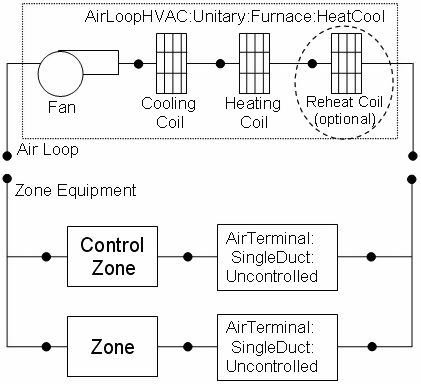
\includegraphics[width=0.9\textwidth, height=0.9\textheight, keepaspectratio=true]{media/image5019.png}
\caption{Schematic of the EnergyPlus Furnace (Blow Through Configuration) \protect \label{fig:schematic-of-the-energyplus-furnace-blow}}
\end{figure}

While the furnace may be configured to serve multiple zones, system operation is controlled by a thermostat located in a single ``control'' zone. One of the key parameters for the furnace component is the fraction of the total system air flow that goes through the control zone. This fraction is calculated as the ratio of the maximum air mass flow rate for the air loop's supply inlet node for the control zone (e.g., AirTerminal:SingleDuct:ConstantVolume:NoReheat, field = Maximum Air Flow Rate, converted to mass flow) to the sum of the maximum air mass flow rates for the air loop's supply inlet nodes for all zones served by this air loop. The furnace module scales the calculated load for the control zone upward based on this fraction to determine the total load to be met by the furnace. The module then proceeds to calculate the required part-load ratio for the system coil and the supply air fan to meet this total load. The heating or cooling capacity delivered by the furnace is distributed to all of the zones served by this system via the terminal units that supply air to each zone. The supply air fraction that goes though the control zone is calculated as follows:

\begin{equation}
Control Zone Air Flow\,Fraction = \frac{{{{\dot m}_{TUMax\,ControlZone}}}}{{\sum\limits_{j = 1}^{NumOfZones} {{{\dot m}_{TUMax\,Zone\,j}}} }}
\end{equation}

where:

\({\dot m_{TUMax\,ControlledZone}}\) is the maximum air mass flow rate for the air loop supply inlet node (terminal unit) for the control zone (kg/s)

\({\dot m_{TUMax\,Zone\,j}}\) is the maximum air mass flow rate for the air loop supply inlet node for the jth zone (kg/s)

\(NumOfZones\) is the number of zones, or number of air loop supply air inlet nodes for all zones served by the air loop.

The furnace component is able to model supply air fan operation in two modes: cycling fan -- cycling coil (i.e., AUTO fan) and continuous fan -- cycling coil (i.e., fan ON). Fan:OnOff must be used to model AUTO fan, while Fan:OnOff or Fan:ConstantVolume can be used to model fan ON. The fan operation mode is specified using a supply air fan operating mode schedule where schedule values of 0 denote cycling fan operation and schedule values other than 0 (a 1 is usually used) denote continuous fan operation. Using this schedule, the furnace fan may be cycled with cooling or heating coil operation or operated continuously based on time of day (e.g., cycling fan operation at night and continuous fan operation during the daytime). If the fan operating mode schedule name field is left blank in the furnace object, the furnace assumes cycling or AUTO fan mode operation throughout the simulation.

The only output variables reported by the furnace object are the fan part-load ratio and the compressor part-load ratio (HeatCool only). The fan part-load ratio is defined as the actual air mass flow rate through the system for the time step divided by the design supply air mass flow rate specified for the furnace (\({{{{\dot m}_{actual}}} \mathord{\left/ {\vphantom {{{{\dot m}_{actual}}} {{{\dot m}_{design}}}}} \right. } {{{\dot m}_{design}}}}\)). The furnace operates based on the user-specified (or autosized) design supply air flow rate(s). The `design' supply air mass flow rate may be different for cooling, heating, and when no cooling or heating is required and the fan operates continuously based on user-specified inputs (HeatCool only). For the HeatCool version, If alternate air flow rates are specified for cooling, heating, and when no cooling or heating is required, the design supply air mass flow rate is the maximum of these specified values. Also for the HeatCool version, the compressor part-load ratio is reported as the ratio of the actual cooling load to the full-load sensible capacity (see Equation~\ref{eq:FurnacePartLoadRatio580}). Reporting of other variables of interest for the furnace (heating rate, cooling rate, energy consumption, etc.) is done by the individual system components (fan, heating coil and DX cooling coil).

\subsubsection{Model Description}\label{model-description-1}

As described previously, the furnace is a ``virtual'' component consisting of a fan, heating coil and, for the HeatCool version, a cooling coil with an optional reheat coil. The sole purpose of the furnace model is to properly coordinate the operation of the various system components. The following sections describe the flow of information within the model for both the HeatOnly and HeatCool configurations, as well as the differences between cycling and continuous supply air fan operation. The last section describes the optional control of high zone humidity with a reheat coil for the HeatCool configuration.

\subsubsection{HeatOnly Configuration}\label{heatonly-configuration}

The HeatOnly configuration consists of an on/off or constant volume fan and an electric or gas heating coil. When the model is first called during an EnergyPlus simulation, all of the input data specified for each furnace in the input data file are read into data structures for use throughout the remainder of the simulation.

For each simulation time step when the performance of a heat-only furnace is being modeled, the first step is to retrieve the heating load required to meet the thermostat setpoint for the ``control'' zone (see Figure~\ref{fig:schematic-of-the-energyplus-furnace-blow}. Schematic of the EnergyPlus Furnace). See the section ``Summary of Predictor-Corrector Procedure'' elsewhere in this document for more details regarding load calculations. Since the furnace may be specified to serve several zones but controlled based on the load calculated for the ``control'' zone, the total heating load to be met by the furnace is determined from the following equation:

\begin{equation}
Furnace~Heating~Load = \frac{{Control~Zone~Heating~Load}}{{Control~Zone~Air~Flow~Fraction}}
\end{equation}

The model then calculates the furnace's sensible heating energy rate delivered to the zones being served when the system runs at full-load conditions and when the heating coil is OFF. If the supply air fan cycles on and off with the heater, then the sensible heating energy rate is zero when the heating coil is OFF. However if the fan is scheduled to run continuously regardless of coil operation, then the sensible heating energy rate will not be zero when the heating coil is OFF. Calculating the sensible heating energy rate involves modeling the supply air fan (and associated fan heat) and the heating coil. For each of these cases (full load and heating coil OFF), the sensible heating energy rate delivered by the furnace is calculated as follows:

\begin{equation}
Full~Heat~Output = (Mass~Flow~Rat{e_{full~load}}){({h_{out,full~load}} - {h_{control~zone}})_{HRmin}} - {\Delta_{sen,full~load}}
\end{equation}

\begin{equation}
No~Heat~Output = (Mass~Flow~Rat{e_{coil~off}}){({h_{out,coil~off}} - {h_{control~zone}})_{HRmin}} - {\Delta_{sen,coil~off}}
\end{equation}

where:

\emph{Mass Flow Rate\(_{full~load}\)} is the air mass flow rate through furnace at full-load conditions (kg/s)

\emph{h\(_{out,full~load}\)} is the enthalpy of air exiting the furnace at full-load conditions (J/kg)

\emph{h\(_{control~zone}\)} is the enthalpy of air in the control zone where thermostat is located (J/kg)

\emph{HR\(_{min}\)} are the enthalpies evaluated at a constant humidity ratio, the minimum humidity ratio of the furnace exiting air or the air in the control zone

\emph{Mass Flow Rate\(_{coil~off}\)} is the air mass flow rate through the furnace with the heating coil OFF (kg/s)

\emph{h\(_{out,coil~off}\)} is the enthalpy of air exiting the furnace with the heating coil OFF (J/kg)

\(\Delta_{sen,full~load}\) is the sensible load difference between the system output node and the zone inlet node at full-load conditions.

\begin{equation}
  \begin{array}{rl}
    \Delta_{sen,full~load} &= \frac{\dot{m}_{Zone~Inlet}}{Frac} \PB{h_{Out,full~load} - h_{Zone~Inlet}}_{HRmin} \\
                           &+ \PB{\dot{m}_{full~load} - \frac{\dot{m}_{Zone~Inlet}}{Frac}} \PB{h_{Out,full~load} - h_{Control~Zone}}_{HRmin}
  \end{array}
\end{equation}

where:

Frac is the control zone air fraction with respect to the system mass flow rate

\(\Delta_{sen,coil~off}\) is the sensible load difference between the system output node and the zone inlet node with the heating coil OFF conditions.

\begin{equation}
  \begin{array}{rl}
    \Delta_{sen,coil~off} &= \frac{\dot{m}_{Zone~Inlet}}{Frac} \PB{h_{Out,coil~off} - h_{Zone~Inlet}}_{HRmin} \\
                           &+ \PB{\dot{m}_{coil~off} - \frac{\dot{m}_{Zone~Inlet}}{Frac}} \PB{h_{Out,coil~off} - h_{Control~Zone}}_{HRmin}
  \end{array}
\end{equation}

With the calculated sensible heating energy rates and the total sensible heating load to be met by the system, the part-load ratio for the furnace is estimated.

\begin{equation}
PartLoadRatio = MAX\left( {0.0,MIN\left( {1.0,\frac{{ABS\left( {FurnaceHeatingLoad - NoHeatOutput} \right)}}{{ABS(FullHeatOutput - NoHeatOutput)}}} \right)} \right)
\end{equation}

The part-load ratio calculated above is used to determine the required heating coil capacity as \(Qheating\,coil = Qdesign\,*PartLoadRatio\) where \emph{Q\(_{design}\)} is the nominal heating coil capacity as specified in the heating coil object. If the fan cycles on and off with the heating coil (i.e., when the supply air fan operating mode schedule values are equal to 0), then this part-load ratio is also used to determine the operating mass flow rate of the furnace as

\begin{equation}
{\dot m_{furnace}} = {\dot m_{design}}*PartLoadRatio
\end{equation}

~If the fan operates continuously (i.e.~fan ON), the operating mass flow rate is specified as \({\dot m_{design}}\) . The furnace's fan and heating coil are then re-simulated to determine the furnace's delivered sensible heating capacity at the above calculated part-load ratio.

\begin{equation}
{Q_{furnace}} = \left( {{{\dot m}_{furnace}}} \right){\left( {{h_{out,actual}} - {h_{control~zone}}} \right)_{HRmin}} - {\Delta_{sen,actual}}
\end{equation}

where:

\({Q_{furnace}}\) is the sensible heating capacity delivered by the furnace (W)

\({\dot m_{furnace}}\) is the air mass flow rate through the furnace (kg/s)

\emph{h\(_{out,\, actual}\)} is the enthalpy of air exiting the furnace (J/kg)

\emph{h\(_{out,\, control\, zone}\)} is the enthalpy of air in the control zone (J/kg)

\emph{HR\(_{min}\)} are the enthalpies evaluated at a constant humidity ratio, the minimum humidity ratio of the furnace exiting air or the air in the control zone

\(\Delta_{sen,actual}\) is the sensible load difference between the system output node and the zone inlet node at the above calculated part-load ratio.

\begin{equation}
  \begin{array}{rl}
    \Delta_{sen,actual} &= \frac{\dot{m}_{Zone~Inlet}}{Frac} \PB{h_{Out,actual} - h_{Zone~Inlet}}_{HRmin} \\
                           &+ \PB{\dot{m}_{furnace} - \frac{\dot{m}_{Zone~Inlet}}{Frac}} \PB{h_{Out,actual} - h_{Control~Zone}}_{HRmin}
  \end{array}
\end{equation}

Since the part-load performance of the heating coil can be non-linear, and the supply air fan heat varies based on heating coil operation for the case of cycling fan/cycling coil (AUTO fan), the final part-load ratio for the heating coil and fan are determined through iterative calculations (successive modeling of the heating coil and fan) until the furnace's heating output matches the heating load to be met within the heating convergence tolerance. The convergence tolerance is fixed at 0.001 and is calculated based on the difference between the load to be met and the furnace's heating output divided by the load to be met.

\begin{equation}
  Tolerance \equiv \frac{FurnaceHeatingLoad - Q_{furnace}}{FurnaceHeatingLoad} \leq 0.001
\end{equation}

If the furnace has been specified with cycling fan/cycling coil (AUTO fan), then the furnace's design air mass flow rate is multiplied by PartLoadRatio to determine the average air mass flow rate for the system simulation time step. The air conditions at nodes downstream of the heating coil represent the full-load (steady-state) values when the coil is operating. If the supply air fan is specified to run continuously (fan ON), then the air mass flow rate remains at the furnace's design air mass flow rate. In this case, the air conditions at nodes downstream of the heating coil are calculated as the average conditions over the simulation time step (i.e., the weighted average of full-load conditions when the coil is operating and inlet air conditions when the coil is OFF).

For the case where the furnace is scheduled to operate with continuous supply air fan operation, but no heating load is required to meet the setpoint temperature in the control zone, the supply air fan model is still called to determine the fan exiting air conditions. The heating coil model is also called, but for the case with no heating load the heating coil model simply passes the inlet air conditions and mass flow rate from its inlet node to its outlet node. The air exiting the heating coil is then sent to the direct air units for distribution to each zone served by the furnace, where the zone heat balance is performed to determine the resulting zone air conditions. The furnace exiting air conditions and energy consumption are calculated and reported by the individual component models (fan and heating coil).

\subsubsection{HeatCool Configuration}\label{heatcool-configuration}

The HeatCool configuration consists of an on/off or constant volume fan, a DX cooling coil, and an electric or gas heating coil. For the cases where a heating load is calculated for the control zone or no heating/cooling load is calculated for the control zone, the model follows nearly identical computational steps as described in the HeatOnly Configuration section above. The only difference is the air mass flow rate during no cooling/heating operation with continuous supply air fan operation can be different from the air mass flow rate during heater operation for the HeatCool configuration. If a cooling load is calculated by EnergyPlus for the control zone, the solution methodology is also virtually identical and is described here for completeness.

If EnergyPlus determines that the furnace must supply cooling to the control zone to meet the zone air temperature setpoint, then the model computes the total sensible cooling load to be met by the furnace based on the control zone sensible cooling load and the fraction of the furnace air flow that goes through the control zone.

\begin{equation}
Furnace~Cooling~Load = \frac{{Control~Zone~Cooling~Load}}{{Control~Zone~Air~Flow~Fraction}}
\end{equation}

If the supply air fan operating mode schedule requests cycling fan operation, the model first checks for the presence of an economizer in the outside air system serving the furnace's air loop (Ref. AirLoopHVAC:OutdoorAirSystem). If an outside air system is not present or if an air-side economizer is not used, the furnace's compressor is used to meet the furnace cooling load. If an air-side economizer is used and is active (i.e., economizer controls indicate that conditions are favorable to increase the outside air flow rate), the furnace will try to meet the cooling load by operating only the supply air fan. If the fan is able to satisfy the furnace cooling load, the compressor remains off for the entire simulation time step. If the operation of the fan alone is unable to meet the entire cooling load, then the compressor is enabled and additional calculations are performed to determine the compressor's part-load ratio.

The model then calculates the furnace's sensible cooling energy rate delivered to the zones being served when the system runs at full-load conditions and when the DX cooling coil is OFF. If the supply air fan cycles with the compressor, then the sensible cooling energy rate is zero when the cooling coil is OFF. However if the fan is configured to run continuously regardless of coil operation, then the sensible cooling energy rate will probably not be zero when the cooling coil is OFF. Calculating the sensible cooling energy rate involves modeling the supply air fan (and associated fan heat), the DX cooling coil, and the heating coil (simply to pass the air properties and mass flow rate from its inlet node to its outlet node). For each of these cases (full load and DX cooling coil OFF), the sensible cooling energy rate delivered by the furnace is calculated as follows:

\begin{equation}
Full~Cool~Output = (Mass~Flow~Rat{e_{full~load}}){({h_{out,full~load}} - {h_{control~zone}})_{HRmin}} - {\Delta_{sen,full~load}}
\end{equation}

\begin{equation}
No~Cool~Output = (Mass~Flow~Rat{e_{coil~off}}){({h_{out,coil~off}} - {h_{control~zone}})_{HRmin}} - {\Delta_{sen,coil~off}}
\end{equation}

where:

\emph{Mass Flow Rate\(_{full~load}\)} is the air mass flow rate through furnace at full-load conditions (kg/s)

\emph{h\(_{out,full~load}\)} is the enthalpy of air exiting the furnace at full-load conditions (J/kg)

\emph{h\(_{control~zone}\)} is the enthalpy of air in the control zone (where thermostat is located) (J/kg)

\emph{HR\(_{min}\)} are the enthalpies evaluated at a constant humidity ratio, the minimum humidity ratio of the furnace exiting air or the air in the control zone

\emph{Mass Flow Rate\(_{coil~off}\)} is the air mass flow rate through the furnace with the cooling coil OFF (kg/s)

\emph{h\(_{out,coil~off}\)} is the enthalpy of air exiting the furnace with the cooling coil OFF (J/kg)

\(\Delta_{sen,full~load}\) is the sensible load difference between the system output node and the zone inlet node at full-load conditions.

\begin{equation}
  \begin{array}{rl}
    \Delta_{sen,full~load} &= \frac{\dot{m}_{Zone~Inlet}}{Frac} \PB{h_{Out,full~load} - h_{Zone~Inlet}}_{HRmin} \\
                           &+ \PB{\dot{m}_{full~load} - \frac{\dot{m}_{Zone~Inlet}}{Frac}} \PB{h_{Out,full~load} - h_{Control~Zone}}_{HRmin}
  \end{array}
\end{equation}
where:

Frac is the control zone air fraction with respect to the system mass flow rate

\(\Delta_{sen,coil~off}\) is the sensible load difference between the system output node and the zone inlet node with the heating coil OFF conditions.

\begin{equation}
  \begin{array}{rl}
    \Delta_{sen,coil~off} &= \frac{\dot{m}_{Zone~Inlet}}{Frac} \PB{h_{Out,coil~off} - h_{Zone~Inlet}}_{HRmin} \\
                           &+ \PB{\dot{m}_{coil~off} - \frac{\dot{m}_{Zone~Inlet}}{Frac}} \PB{h_{Out,coil~off} - h_{Control~Zone}}_{HRmin}
  \end{array}
\end{equation}

With the calculated sensible cooling energy rates and the total sensible cooling load to be met by the system, the part-load ratio for the furnace is estimated.

\begin{equation}
PartLoadRatio = MAX\left( {0.0,\frac{{ABS\left( {FurnaceCoolingLoad - NoCoolOutput} \right)}}{{ABS\left( {FullCoolOutput - NoCoolOutput} \right)}}} \right)
\label{eq:FurnacePartLoadRatio580}
\end{equation}

Since the part-load performance of the DX cooling coil is frequently non-linear (Ref: DX Cooling Coil Model), and the supply air fan heat varies based on cooling coil operation for the case of cycling fan/cycling coil (AUTO fan), the final part-load ratio for the cooling coil compressor and fan are determined through iterative calculations (successive modeling of the cooling coil and fan) until the furnace's cooling output matches the cooling load to be met within the convergence tolerance. The convergence tolerance is fixed at 0.001 and is calculated based on the difference between the load to be met and the furnace's cooling output divided by the load to be met.

\begin{equation}
  Tolerance \equiv \frac{FurnaceHeatingLoad - Q_{furnace}}{FurnaceHeatingLoad} \leq 0.001
\end{equation}

where \({Q_{furnace}}\) is the furnace delivered sensible capacity (W).

If the furnace has been specified with cycling fan/cycling coil (AUTO fan) and high humidity control \emph{has not} been specified, then the furnace's operating supply air mass flow rate is multiplied by PartLoadRatio to determine the average air mass flow rate for the system simulation time step. The air conditions at nodes downstream of the cooling coil represent the full-load (steady-state) values when the coil is operating. If a cycling fan is used and high humidity control \emph{has} been specified, the calculation of average air mass flow rate is based on the greater of the heating or cooling part-load ratio (see following section on high humidity control). When the heating part-load ratio is greater than the cooling part-load ratio, the air conditions at nodes downstream of the cooling coil represent the weighted average of full-load conditions when the cooling coil is operating and inlet air conditions when the cooling coil is off (i.e., the fan continues to operate due to a heating requirement where the heating PLR is greater than the cooling PLR). If the supply air fan is specified to run continuously (fan ON), then the air mass flow rate continues to operate at the user-specified supply air mass flow rate when no cooling or heating is required. In this case, the air conditions at nodes downstream of the cooling coil are calculated as the average conditions over the simulation time step (i.e., the weighted average of full-load conditions when the coil is operating and inlet air conditions when the coil is OFF). The furnace exiting air conditions and energy consumption are calculated and reported by the individual component models (fan and DX cooling coil).

\subsubsection{High Humidity Control with HeatCool Configuration}\label{high-humidity-control-with-heatcool-configuration}

An optional reheat coil can be specified with the HeatCool configuration to allow the furnace to control high zone humidity levels. The specific configuration of the HeatCool Furnace with high humidity control option is shown in Figure~\ref{fig:schematic-for-blow-through-furnace-with-high}. The figure below shows the fan placement when a blow through fan is specified. If a draw through fan is specified, the fan is located between the heating coil and the reheat coil. The system is controlled to keep the relative humidity in the control zone from exceeding the setpoint specified in the object ZoneControl:Humidistat. This option is available when the supply air fan operates continuously (i.e., the supply air fan operating mode schedule values are never equal to 0) or the supply air fan cycles with the compressor. For the case of cycling fan mode when the high humidity control is specified as CoolReheat \emph{and} the heating part-load ratio is greater than the compressor part-load ratio, the air conditions at nodes downstream of the cooling coil are calculated as the average conditions during the duration of fan operation (i.e., the weighted average of full load conditions when the coil is operating and inlet air conditions when the coil is off and the fan continues to operate to meet the heating load). For the case where cycling fan mode is used \emph{and} the heating part-load ratio is less than the compressor part-load ratio, the air conditions at the nodes downstream of the cooling coil are simply the full load (steady-state) values when the coil is operating. In addition, when high humidity control is specified and the compressor operates, the furnace operates at the cooling air flow rate when a zone heating load is present as determined by the zone thermostat.

High humidity control is specified as either None, MultiMode, or CoolReheat in the Dehumidification Control Type input field. MultiMode is specified when a heat exchanger is used to improve the dehumidification performance of the cooling coil. The heat exchanger will be activated when the sensible part-load ratio is insufficient to meet the zone latent load. CoolReheat is specified when a DX cooling coil is used to over-cool the supply air stream in order to meet the zone latent load. In this case, a reheat coil will ensure the zone temperature does not fall below the zone heating temperature set point. When a heat exchanger is used in conjunction with a DX cooling coil and CoolReheat is specified as the Dehumidification Control Type, the heat exchanger is ``locked on'' to meet either the sensible or latent cooling load. If the dehumidification control type is selected as None and a heat exchanger assisted cooling coil is used, the heat exchanger is ``locked on'' and the air conditioner runs only to meet the sensible cooling load. Although a reheat coil is required when CoolReheat is specified in the Dehumidification Control Type input field, this reheat coil may optionally be present for the other Dehumidification Control Types (e.g., None and Multimode). If the reheat coil is present and the dehumidification control type input is not specified as CoolReheat, the reheat coil will not be active. This allows changing the dehumidification control option without requiring a change in the unit's coil configuration.

The model first calculates the PartLoadRatio required to meet the sensible cooling load as described above (see Equation~\ref{eq:FurnacePartLoadRatio580}) to maintain the dry-bulb temperature setpoint in the control zone. If a moisture (latent) load exists because the control zone humidity has exceeded the setpoint, the total moisture load to be met by the HeatCool furnace (SystemMoistureLoad) is calculated based on the control zone moisture load and the control zone air flow fraction. The model then calculates the LatentPartLoadRatio required to meet the humidistat setpoint.

\begin{equation}
SystemMoistureLoad = \frac{{Control~Zone~Moisture~Load}}{{Control~Zone~Air~Flow~Fraction}}
\end{equation}

\begin{equation}
LatentPartLoadRatio = MAX\left( {MinPLR,\frac{{ABS\left( {SystemMoistureLoad - NoLatentOutput} \right)}}{{ABS\left( {FullLatentOutput - NoLatentOutput} \right)}}} \right)
\end{equation}

where:

\emph{FullLatentOutput} is the furnace's latent cooling energy rate at full-load conditions (W)

\emph{NoLatentOutput} is the furnace's latent cooling energy rate with the cooling coil OFF (W)

\emph{MinPLR} is the minimum part-load ratio, which is usually 0.0. For the case when the latent capacity degradation model is used (Ref: DX Cooling Coil Model), this value is the minimum part-load ratio at which the cooling coil will dehumidify the air.

The model uses the greater of the two part-load ratios, PartLoadRatio or LatentPartLoadRatio, to determine the operating part-load ratio of the furnace's DX cooling coil. As previously described, iterations are performed to converge on the solution within the convergence tolerance.

\begin{figure}[hbtp] % fig 222
\centering
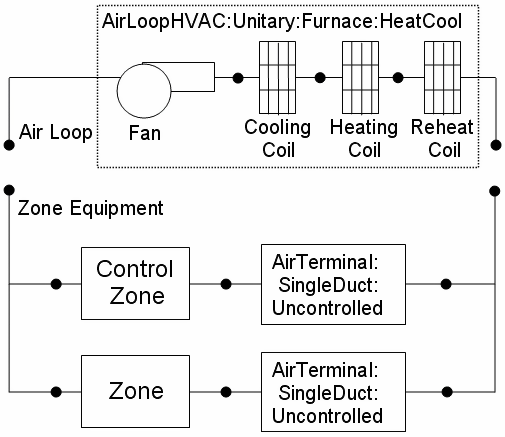
\includegraphics[width=0.9\textwidth, height=0.9\textheight, keepaspectratio=true]{media/image5049.png}
\caption{Schematic for Blow Through Furnace with High Humidity Control \protect \label{fig:schematic-for-blow-through-furnace-with-high}}
\end{figure}

If the model determines that the LatentPartLoadRatio is to be used as the operating part-load ratio of the furnace's cooling coil, the reheat coil is used to offset the excess sensible capacity provided by the unit. The model first checks the sensible load that exists for the current simulation time step (predicted zone temperature with no HVAC operation compared to the thermostat setpoint temperatures). If a sensible cooling load or no sensible cooling or heating load exists (Figure~\ref{fig:reheat-coil-load-when-predicted-zone}), the model calculates the difference between the sensible heating load required to reach or maintain the heating dry-bulb temperature setpoint and the actual sensible cooling energy rate delivered by the unit (with LatentPartLoadRatio). In this case, the reheat coil is used to offset the excess sensible cooling energy provided by the DX cooling coil (if any) that could have caused an overshoot of the heating dry-bulb temperature setpoint. Note that when a humidistat is used and high humidity control is required, the zone dry-bulb temperature will typically move toward the heating temperature setpoint when a high moisture (latent) load exists. If a heating load exists (Figure~\ref{fig:reheat-coil-load-when-predicted-zone-001}), the reheat coil is used to offset the entire sensible cooling energy rate of the DX cooling coil (to meet the humidistat setpoint) and the heating coil is used to meet the entire heating load as described in the HeatOnly configuration section above. Note that when a heating load exists and high humidity control is required, the furnace operates at the user-specified cooling air flow rate for the entire simulation time step. As with the fan, DX cooling coil, and heating coil, report variables associated with reheat coil performance (e.g., heating coil energy, heating coil rate, heating coil gas or electric consumption, heating coil runtime fraction, etc.) are managed in the reheat (heating) coil object.

\begin{figure}[hbtp] % fig 223
\centering
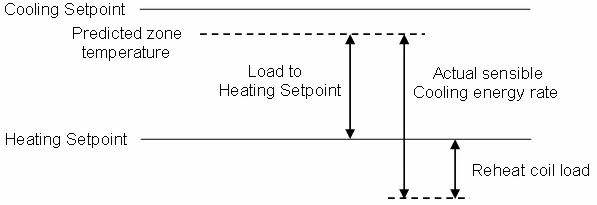
\includegraphics[width=0.9\textwidth, height=0.9\textheight, keepaspectratio=true]{media/image5050.png}
\caption{Reheat Coil Load when Predicted Zone Temperature is Above Heating Setpoint \protect \label{fig:reheat-coil-load-when-predicted-zone}}
\end{figure}

\begin{figure}[hbtp] % fig 224
\centering
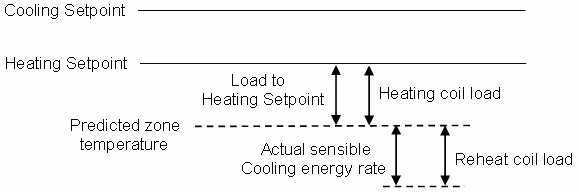
\includegraphics[width=0.9\textwidth, height=0.9\textheight, keepaspectratio=true]{media/image5051.png}
\caption{Reheat Coil Load when Predicted Zone Temperature is Below Heating Setpoint \protect \label{fig:reheat-coil-load-when-predicted-zone-001}}
\end{figure}

\subsection{Unitary Systems}\label{unitary-systems-1}

The input objects AirLoopHVAC:UnitaryHeatCool and AirLoopHVAC:UnitaryHeatOnly provides models that are identical to the Furnace and Central Air models described above.~ Please reference the previous section for details.

\subsection{Unitary System with Changeover-Bypass-Variable Air Volume}\label{unitary-system-with-changeover-bypass-variable-air-volume}

\subsubsection{Overview}\label{overview-2}

The input object AirLoopHVAC:UnitaryHeatCool:VAVChangeoverBypass provides a model for a changeover-bypass variable air volume (CBVAV) unitary system that is a compound object made up of other components. Each CBVAV system consists of an outside air mixer, direct expansion (DX) cooling coil, heating coil, and a supply air fan as shown in the figures below. Zone thermostats and terminal units are required in each zone served by this system. The terminal units are specific to this system type and are either AirTerminal:SingleDuct:VAV:HeatAndCool:Reheat or AirTerminal:SingleDuct:VAV:HeatAndCool:NoReheat. A zone humidistat and single zone max humidity setpoint manager may also be specified to help control high humidity levels. These individual components are described elsewhere in this document. The CBVAV unitary system object coordinates the operation of these components and is modeled as a type of air loop equipment (Ref. AirLoopHVAC).

\begin{figure}[hbtp] % fig 225
\centering
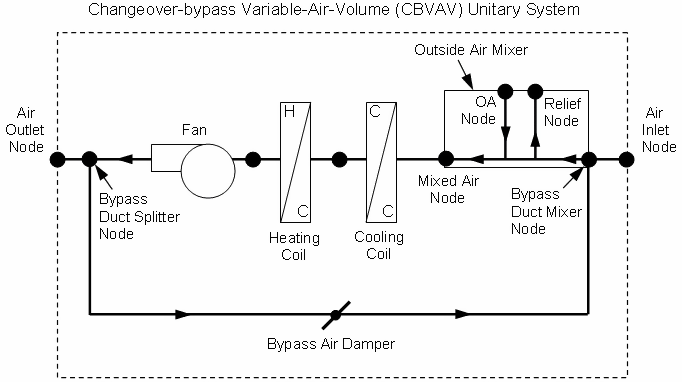
\includegraphics[width=0.9\textwidth, height=0.9\textheight, keepaspectratio=true]{media/image5052.png}
\caption{Schematic of a Changeover Bypass VAV Unitary System with Draw Through Fan \protect \label{fig:schematic-of-a-changeover-bypass-vav-unitary}}
\end{figure}

\begin{figure}[hbtp] % fig 226
\centering
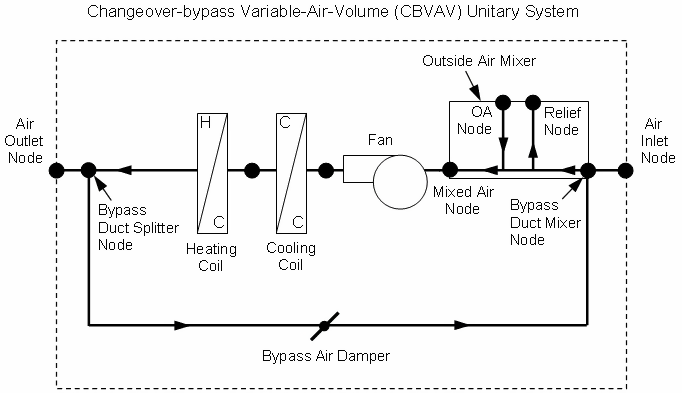
\includegraphics[width=0.9\textwidth, height=0.9\textheight, keepaspectratio=true]{media/image5053.png}
\caption{Schematic of Changeover Bypass VAV Unitary System with Blow Through Fan \protect \label{fig:schematic-of-changeover-bypass-vav-unitary}}
\end{figure}

The CBVAV unitary system conditions one or more zones and is controlled by thermostats located in each zone (the use of a single humidistat is also allowed when using multi-mode DX cooling coils). The CBVAV system operates to meet the zone sensible cooling or sensible heating requirements as dictated by the thermostat schedule(s). The priority control input determines the mode of operation and is specified as Cooling Priority, Heating Priority, or Zone Priority. If Cooling Priority is specified, the system operates to meet the cooling load when any zone served by this system (air loop) requires cooling. If Heating Priority is specified, the system operates to meet the heating load when any zone requires heating. If Zone Priority is specified, the system operates based on the maximum number of zones requiring either heating or cooling.

Once the operating mode is determined, the CBVAV model calculates a target supply air temperature required to operate a single terminal unit at its maximum air flow rate. The remaining terminal units will modulate as required to maintain the dry-bulb temperature in the zone they are serving according to the thermostat schedule for their respective zone. The system air flow rate (through the supply air fan, cooling coil and heat coil) remains constant during cooling operation, heating operation, and no cooling/heating mode as specified by the user. Therefore, as the zone terminal units modulate to reduce zone air flow rates, the excess system air flow is ``bypassed'' from the bypass duct splitter node back to the bypass duct mixer node of the CBVAV system (see figures above).

The CBVAV system is able to model supply air fan operation in two modes: cycling fan -- cycling coil (i.e., AUTO fan) and continuous fan -- cycling coil (i.e., fan ON). A Fan:OnOff or Fan:ConstantVolume is used in either case. Since the excess system air flow is bypassed while the zone terminal units modulate, the supply air fan operates the entire simulation time step when heating or cooling is required. For this reason, AUTO fan only allows the supply air fan to turn off when no cooling or heating is required. If fan ON is specified, the supply air fan runs the entire time the system is scheduled to operate (via its availability schedule). The mode of operation for the supply air fan is specified through a fan operating mode schedule where a value of 0 in the schedule indicates cycling fan mode and a value greater than 0 indicates continuous fan mode. If the schedule is not provided, the supply air fan operating mode is considered to be continuous (fan ON).

Output variables reported for the CBVAV system include the supply air fan part-load ratio, the compressor part-load ratio, and the electric consumption of the CBVAV system. Additional output variables report the total heating rate and total cooling rate provided by the CBVAV system. The sensible and latent components for total system cooling and heating are also available as output variables. Reporting of other variables of interest for the CBVAV system (DX coil cooling rate, heating rate, crankcase electric power and energy, supply air fan electric power, etc.) is done by the individual system components (fan, DX cooling coil, and heating coil).

\subsubsection{Model Description}\label{model-description-2}

As described previously, the CBVAV system conditions one or more zones and is controlled by zone thermostats (Ref. ZoneControl:Thermostat). For each simulation time step, EnergyPlus performs a zone air heat balance to determine if cooling or heating is required to meet the zone thermostat setpoints, excluding any impacts from CBVAV system operation. CBVAV system performance is then modeled with all heating/cooling coils off but with the supply air fan operating according to the user specified supply air fan operating mode schedule. If the zone air heat balance plus the impact of CBVAV system operation with coils off results in no requirement for heating or cooling by the CBVAV coils, or if the CBVAV system is scheduled off (via its availability schedule), then the CBVAV coils do not operate and the compressor part-load ratio output variable is set to 0. If the model determines that cooling or heating is required and the CBVAV system is scheduled to operate, the model calculates a target supply air temperature required to maintain a single terminal unit at it's maximum air flow rate, the amount of bypass air returning to the bypass duct mixer node, and the part-load ratio of the cooling or heating coils in order to meet the target supply air temperature.

When high humidity control is desired, a ZoneControl:Humidistat input object and a SetpointManager:SingleZone:Humidity:Maximum, SetpointManager:MultiZone:MaximumHumidity:Average~ ~~or SetpointManager:MultiZone:Humidity:Maximum object are required. The air outlet node of the CBVAV system is used as the control node for the setpoint manager. For this reason, only a single humidistat should be specified for one of the zones being served by this system. If humidistat/setpoint manager objects are specified for more than one zone served by this system, only the last of the SetpointManager:SingleZone:Humidity:Maximum objects is used (the setpoint manager objects are read in order of occurrence in the input file). Since the outlet node of the CBVAV system is always used as the control node, the setpoints calculated by the previous setpoint managers are overwritten by the last setpoint manager in the input. When a heat exchanger is used to improve the dehumidification performance of the cooling coil (i.e.~CoilSystem:Cooling:DX:HeatExchangerAssisted), the heat exchanger is always active and can not be turned on and off based on zone humidity levels.

The remainder of this section describes the calculations performed when cooling or heating coil operation is required. For any HVAC simulation time step, the CBVAV system can only cool or heat the air, not both. Because the CBVAV system bypasses system air flow back to the inlet of the CBVAV unit, the system operates for the entire simulation time step. If the user specifies continuous fan operation, then the supply air fan continues to operate at a user-specified flow rate even during periods when the coils cycle off. If the user specifies AUTO fan operation, then the supply air fan cycles off for the entire simulation time step only when no cooling or heating is required.

\paragraph{Operating Mode}\label{operating-mode}

The first step in modeling a CBVAV system is to obtain the cooling or heating load for each zone as calculated by EnergyPlus based on the zone thermostat setpoint temperature(s). The calculated loads for each zone are used to determine the total cooling and heating requirements for all zones served by this system. In addition to summing the zone cooling and heating loads, the number of zones in cooling and the number of zones in heating are totalized. The priority control mode specified by the user is then used to determine the operating mode for this simulation time step.

If Cooling Priority is specified and the total cooling requirement in all zones is not equal to zero, then cooling is selected as the operating mode. If the total cooling requirement is equal to zero and the total heating requirement is not equal to zero, then heating is selected as the operating mode. If the total cooling requirement and total heating requirement are equal to zero then the zones are allowed to float (no heating or cooling provided).

If Heating Priority is specified and the total heating requirement in all zones is not equal to zero, then heating is selected as the operating mode. If the total heating requirement is equal to zero and the total cooling requirement is not equal to zero, then cooling is selected as the operating mode. If the total cooling requirement and total heating requirement are equal to zero then the zones are allowed to float (no heating or cooling provided).

If Zone Priority is specified and the total number of zones requiring cooling is greater than the total number of zones requiring heating, then cooling is selected as the operating mode. If the total number of zones requiring heating is greater than the total number of zones requiring cooling, then heating is selected as the operating mode. If the total number of zones requiring cooling is equal to the total number of zones requiring heating, then the magnitude of the total cooling and heating requirements for all zones sets the operating mode. In this case, if the magnitudes of the cooling and heating requirements are zero, then the zones are allowed to float (no heating or cooing provided). If the magnitudes of the cooling and heating requirements are non-zero and identical, then cooling is selected as the operating mode.

\paragraph{Calculation of Bypass Duct Mixer Node Conditions}\label{calculation-of-bypass-duct-mixer-node-conditions}

The operation of this system is unique in that it uses constant-air-volume equipment to provide variable air volume to the conditioned zones. This is accomplished with the use of a bypass duct (shown in the figures above) which shunts excess system air flow from the bypass duct splitter node at the system's outlet back to the bypass duct mixer node at the system's inlet. The air conditions at the bypass duct mixer node are based on the inlet air to the CBVAV system, the system outlet air conditions required to meet the zone loads, and the fraction of bypassed air. The following calculations are performed each simulation time step.

\begin{equation}
BypassFrac = 1.0 - \left( {\frac{{{{\dot m}_{supply}}}}{{{{\dot m}_{system}}}}} \right)
\end{equation}

\begin{equation}
{T_{bypassductmixernode}} = \left( {1 - BypassFrac} \right){T_{inlet}} + \left( {BypassFrac} \right){T_{outlet}}
\end{equation}

\begin{equation}
{\omega_{bypassductmixernode}} = \left( {1 - BypassFrac} \right){\omega_{inlet}} + \left( {BypassFrac} \right){\omega_{outlet}}
\end{equation}

\begin{equation}
{h_{bypassductmixernode}} = PsyHFnTdbW\left( {{T_{mixerinlet}},{\omega_{mixerinlet}}} \right)
\end{equation}

where:

\(BypassFrac\) is the fraction of system air directed to the bypass duct mixer node

\({\dot m_{supply}}\) is the air mass flow rate at the system's air outlet node (kg/s)

\({\dot m_{system}}\) is the air mass flow rate through the CBVAV system including the coils and supply air fan (kg/s)

\({T_{bypassductmixernode}}\) is the air temperature at the bypass duct mixer node (\(^{\circ}\)C)

\({T_{inlet}}\) is the air inlet node temperature (\(^{\circ}\)C)

\({T_{outlet}}\) is the air outlet node temperature (\(^{\circ}\)C)

\({\omega_{bypassductmixernode}}\) is the air humidity ratio at the bypass duct mixer node (kg/kg)

\({\omega_{inlet}}\) is the air inlet node humidity ratio (kg/kg)

\({\omega_{outlet}}\) is the air outlet node humidity ratio (kg/kg)

\({h_{bypassductmixernode}}\) is the air enthalpy at the bypass duct mixer node (J/kg)

\(PsyHFnTdbW\) is an EnergyPlus psychrometric function calculating enthalpy given dry-bulb temperature and humidity ratio.

\paragraph{Cooling Operation}\label{cooling-operation}

If the model determines that the CBVAV system must supply cooling to the zones, the model first calculates a target outlet air dry-bulb temperature required to operate a single terminal unit at its maximum air flow rate. The minimum target temperature for all zones is used to control the CBVAV system in cooling mode.

\begin{equation}
  T_{target}^i = T_{Zone}^i + \frac{Q_{Zone}^i}{\dot{m}_{zone,max}^i C_p};~~~~i = 1,n
\end{equation}

\begin{equation}
{T_{target}} = MIN\left( {T_{target}^i} \right);~~~~i = 1,n
\end{equation}

where:

\(T_{target}^i\) is the target supply air temperature for zone \emph{i} (\(^{\circ}\)C)

\(T_{zone}^i\) is the air temperature in zone \emph{i} (\(^{\circ}\)C)

\(Q_{zone}^i\) is the cooling or heating load for zone \emph{i} where cooling loads are negative values and heating loads are positive values (W)

\(Cp\) is the specific heat of supply air with coils off (J/kg-K)

\(\dot m_{zone,max}^i\) is the maximum terminal unit mass flow rate in zone \emph{i} (kg/s)

\(T_{target}^{}\) is the target supply (outlet) air temperature for the CBVAV system (\(^{\circ}\)C).

The model then calculates the part-load ratio of the DX compressor required to meet the target supply (outlet) air temperature. Since the part-load performance of the DX cooling coil is frequently non-linear (Ref: Coil:Cooling:DX:SingleSpeed model), the actual part-load ratio for the cooling coil compressor is determined through iterative calculations (successive modeling of the DX cooling coil model) until the CBVAV system's outlet air temperature (including on/off cycling effects of the DX coil) matches the target supply (outlet) air temperature within a small temperature convergence tolerance (1E-5\(^{\circ}\)C).

Since the supply air fan operates continuously for each simulation time step (or is OFF for the entire HVAC system time step), the air conditions at nodes downstream of the cooling coil are calculated as the average conditions over the simulation time step (i.e., the weighted average of coil's outlet node conditions when the coil is operating and the coil's inlet node conditions when the coil is OFF).

\paragraph{Heating Operation}\label{heating-operation}

Modeling the CBVAV system's DX heating coil is identical to the calculations described above for cooling operation except that the maximum target supply air temperature for all zones is used to control the CBVAV system in heating mode.

\begin{equation}
{T_{target}} = MAX\left( {T_{target}^i} \right);~~~~i = 1,n
\end{equation}

Iterative calculations (successive modeling of the DX heating coil model) are used to determine the final heating coil part-load ratio to account for the non-linear performance of the DX heating coil at part-load conditions.

When a gas or electric heating coil is used instead of a DX heating coil, the amount of heat required by the coil is calculated based on the target supply (outlet) air temperature and the coil inlet air temperature as follows:

\begin{equation}
{Q_{heating}} = {\dot m_{system}}{C_p}({T_{target}} - {T_{inlet,heatcoil}})
\end{equation}

where:

\({Q_{heating}}\) is the heating coil load (W)

\({C_p}\) is the specific heat of heating coil inlet air (J/kg-K)

\({T_{inlet,heatcoil}}\) is the heating coil inlet air temperature (\(^{\circ}\)C).

\paragraph{Floating Operation (no cooling or heating)}\label{floating-operation-no-cooling-or-heating}

When the zone thermostats determine that there is no cooling or heating requirement in any zone, the CBVAV coils are OFF and the zone temperatures are allowed to float. However, a special case exists where the user specifies continuous supply air fan operation and no cooling or heating requirements exist in any zone. In this case, the outlet air temperature of the CBVAV system (with fan ON and coils OFF) is compared to the target outlet air temperatures required to maintain the zone's cooling and heating setpoint temperatures. If the outlet air temperature with the supply fan ON and coils OFF is below the target outlet air temperature required to maintain the heating setpoint, then heating mode is enabled to avoid overshooting the zone heating setpoint temperature. Conversely, if the outlet air temperature with the supply fan ON and coils OFF is above the target outlet air temperature required to maintain the cooling setpoint, then cooling mode is enabled to avoid overshooting the zone cooling setpoint temperature. This special case is handled at any time a no load condition is reported by the thermostats and overshooting the zone air temperature setpoint is possible regardless of the priority control mode selected by the user.

\paragraph{Minimum and Maximum Outlet Air Temperature in Cooling/Heating Operation}\label{minimum-and-maximum-outlet-air-temperature-in-coolingheating-operation}

The user also specifies a minimum outlet air temperature during cooling operation and a maximum outlet air temperature during heating operation. The target outlet air temperature, as calculated above, is compared to each of these limits during each simulation time step. The resulting target outlet air temperature is used to control the heating and cooling coils.

\begin{equation}
{T_{target}} = MAX\left( {{T_{target}},{T_{min,cooling}}} \right)
\end{equation}

\begin{equation}
{T_{target}} = MIN\left( {{T_{target}},{T_{max,heating}}} \right)
\end{equation}

where:

\({T_{min,cooling}}\) is the minimum outlet air temperature during cooling operation (\(^{\circ}\)C)

\({T_{max,heating}}\) is the maximum outlet air temperature during heating operation (\(^{\circ}\)C).

\paragraph{Air Flow Calculations}\label{air-flow-calculations}

The changeover-bypass VAV system operates based on user-specified (or autosized) air flow rates. The CBVAV system air flow rate (i.e., air flow through the supply air fan and heating/cooling coils) during cooling operation may be different than the system air flow rate during heating operation. In addition, the system air flow rate when no cooling or heating is required but the supply air fan remains ON can be different than the air flow rates when cooling or heating is required. The outside air flow rates can likewise be different in these various operating modes. The model takes these different air flow rates into account when simulating the performance of the CBVAV system. The system air flow rate for each simulation time step is based on the current operating mode (cooling, heating, or no cooling/heating) and is reported on the inlet/outlet air nodes of the various CBVAV components (e.g.~fan, cooling coil, and heating coil). The supply air flow rate delivered to the individual zones is calculated based on the sum of the air flow rates through each terminal unit and is reported at the air inlet and outlet nodes of the CBVAV system each simulation time step. The difference between the system air mass flow rate and the supply air mass flow rate delivered to all zones is equal to the bypass air mass flow rate which is also reported each simulation time step.

The system and outside air flow rates when a system coil is ON (e.g., system air volumetric flow rate during cooling operation, system air volumetric flow rate during heating operation, outside air volumetric air flow rate during cooling operation, and outside air volumetric air flow rate during heating operation) or the system coils are OFF and the fan operates continuously (e.g., system air volumetric flow rate when no cooling or heating is needed and outside air volumetric air flow rate when no cooling or heating is needed) are specified by the user, or can be autosized, and are converted from volumetric flow rate to mass flow rate at standard conditions. If the user has specified cycling fan operation, then the system air and outside air mass flow rates when the system coils are OFF the entire time step are zero. If the user has specified constant fan operation, then the air flow rates when no cooling or heating is needed are used when the system coils are OFF the entire time step.

There is one special case. If the user has specified constant fan operation and they specify that the system air volumetric flow rate when no cooling or heating is needed is zero (or if the field is left blank), then the model assumes that the system air mass flow rate when the system coils are OFF the entire time step is equal to the corresponding air mass flow rate when any system coil was last operating (ON). This model handles the zero (or blank) entry for outside air volumetric flow rate when no cooling or heating is needed in an analogous fashion.

\begin{equation}
{\dot m_{system}} = {\rho_{air,std}}*{\dot V_{mode}}
\end{equation}

\begin{equation}
{\dot m_{system,OA}} = {\rho_{air,std}}*{\dot V_{mode,OA}}
\end{equation}

\begin{equation}
{\dot m_{supply}} = \sum\limits_{i = 1}^n {{{\dot m}_{zone}}}
\end{equation}

\begin{equation}
{\dot m_{bypass}} = {\dot m_{system}} - {\dot m_{supply}}
\end{equation}

where:

\({\rho_{air,std}}\) is the standard air density (1.204 kg/m\(^{3}\)) adjusted for the local barometric pressure (standard barometric pressure corrected for altitude, ASHRAE 1997 HOF pg. 6.1)

\({\dot V_{mode}}\) is the user-specified system volumetric flow rate in cooling, heating, or no cooling or heating mode (m\(^{3}\)/s)

\({\dot m_{system,OA}}\) is the outdoor air mass flow rate introduced through the CBVAV system (kg/s)

\({\dot V_{mode,OA}}\) is the user-specified outdoor air volumetric flow rate in cooling, heating, or no cooling or heating mode (m\(^{3}\)/s).

\paragraph{Calculation of System Heating and Cooling Rates}\label{calculation-of-system-heating-and-cooling-rates}

At the end of each HVAC simulation time step, this object reports the heating or cooling rate and energy delivered by the system, as well as the electric power and consumption by the system. In terms of thermal energy delivered by the system, the sensible, latent and total energy transfer rates for the system are calculated as follows:

\begin{equation}
{\dot Q_{total}} = ({\dot m_{supply}})({h_{outlet}} - {h_{inlet}})
\end{equation}

\begin{equation}
{\dot Q_{sensible}} = ({\dot m_{supply}}){({h_{outlet}} - {h_{inlet}})_{HRmin}}
\end{equation}

\begin{equation}
{\dot Q_{latent}} = {\dot Q_{total}} - {\dot Q_{sensible}}
\end{equation}

where:

\(\dot{Q}_{total}\) is the total energy transfer rate by the system (W)

\(\dot{Q}_{sensible}\) is the sensible energy transfer rate by the system (W)

\(\dot{Q}_{latent}\) is the latent energy transfer rate by the system (W)

\emph{h\(_{inlet}\)} is the enthalpy of the air entering the unit at its inlet node (J/kg)

\emph{h\(_{outlet}\)} is the enthalpy of the air leaving the unit at its outlet node (J/kg)

\(H{R_{min}}\) is the minimum of the inlet air and outlet air humidity ratio (kg/kg).

Since each of these energy transfer rates can be calculated as positive or negative values, individual reporting variables are established for cooling and heating and only positive values are reported. The following calculations are representative of what is done for each of the energy transfer rates:

If $\dot{Q}_{total}<0$, then:

\begin{equation}
  \begin{array}{rl}
    \dot{Q}_{total,cooling} &= \left|\dot{Q}_{total}\right| \\
    \dot{Q}_{total,heating} &= 0
  \end{array}
\end{equation}

Else:

\begin{equation} 
  \begin{array}{rl}
    \dot{Q}_{total,cooling} &= 0.0 \\
    \dot{Q}_{total,heating} &= \dot{Q}_{total}
  \end{array}
\end{equation}

where:

\(\dot{Q}_{total,cooling}\) is the output variable `Unitary System Total Cooling Rate, W'

\(\dot{Q}_{total,heating}\) is the output variable `Unitary System Total Heating Rate, W'.

In addition to heating and cooling rates, the heating and cooling energy supplied by the system are also calculated for the time step being reported. The following example for total zone cooling energy is representative of what is done for the sensible and latent energy as well as the heating counterparts.

\begin{equation}
{Q_{total,cooling}} = {\dot Q_{total,cooling}}*TimeStepSys*3600
\end{equation}

where:

\(Q_{total,cooling}\) is the output variable `Unitary System Total Cooling Energy, J'

\emph{TimeStepSys} is the HVAC system simulation time step (hr)

3600 is a conversion factor (sec/hr).

\subsubsection{Changeover-bypass VAV Unitary System Sizing}\label{changeover-bypass-vav-unitary-system-sizing}

The changeover-bypass VAV system is modeled as an air loop component and is sized according to the methodology described elsewhere in this document (Ref. System Design Loads and Air Flow Rates). The following volumetric air flow rates may be autosized:

\begin{itemize}
\item System air volumetric flow rate during cooling operation
\item System air volumetric flow rate during heating operation
\item System air volumetric flow rate when no cooling or heating is needed
\item Outside air volumetric air flow rate during cooling operation
\item Outside air volumetric air flow rate during heating operation
\item Outside air volumetric air flow rate when no cooling or heating is needed
\end{itemize}

\subsection{Unitary Air-To-Air Heat Pump}\label{unitary-air-to-air-heat-pump}

\subsubsection{Overview}\label{overview-3}

The input object AirLoopHVAC:UnitaryHeatPump:AirToAir provides a model for an air-to-air heat pump that is a ``virtual'' component that consists of an on/off or constant volume fan component, a DX cooling coil, a DX heating coil, and a gas or electric supplemental heating coil. The specific configuration of the blow through heat pump is shown in the following figure. For a draw through heat pump, the fan is located between the DX heating coil and the supplemental heating coil.

\begin{figure}[hbtp] % fig 227
\centering
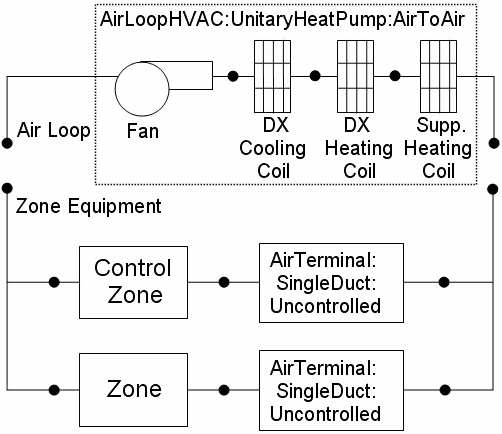
\includegraphics[width=0.9\textwidth, height=0.9\textheight, keepaspectratio=true]{media/image5106.png}
\caption{Schematic of a Blow Through Air-to-Air Heat Pump \protect \label{fig:schematic-of-a-blow-through-air-to-air-heat}}
\end{figure}

While the heat pump may be configured to serve multiple zones, system operation is controlled by a thermostat located in a single ``control'' zone. One of the key parameters for the heat pump component is the fraction of the total system airflow that goes through the control zone. This fraction is calculated as the ratio of the maximum air mass flow rate for the air loop's supply inlet node for the control zone (e.g., AirTerminal:SingleDuct:ConstantVolume:NoReheat, field = Maximum Air Flow Rate, converted to mass flow) to the sum of the maximum air mass flow rates for the air loop's supply inlet nodes for all zones served by this air loop. The heat pump module scales the calculated load for the control zone upward based on this fraction to determine the total load to be met by the heat pump. The module then proceeds to calculate the required part-load ratio for the system coil and the supply air fan to meet this total load. The heating or cooling capacity delivered by the heat pump is distributed to all of the zones served by this system via the direct air units that supply air to each zone. The supply air fraction that goes though the control zone is calculated as follows:

\begin{equation}
Control~Zone~Air~Flow~Fraction = \frac{{{{\dot m}_{TUMax~ControlZone}}}}{{\sum\limits_{j = 1}^{NumOfZones} {{{\dot m}_{TUMax~Zone~j}}} }}
\end{equation}

where:

\({\dot m_{TUMax~ControlledZone}}\) is the maximum air mass flow rate for the air loop's supply inlet node (terminal unit) for the control zone (kg/s)

\({\dot m_{TUMax~Zone~j}}\) is the maximum air mass flow rate for the air loop's supply inlet node for the jth zone (kg/s)

\(NumOfZones\) is the number of zones, or number of air loop supply air inlet nodes for all zones served by the air loop.

The heat pump component is able to model supply air fan operation in two modes: cycling fan -- cycling coil (i.e., AUTO fan) and continuous fan -- cycling coil (i.e., fan ON). Fan:OnOff must be used to model AUTO fan, while Fan:OnOff or Fan:ConstantVolume can be used to model fan ON. The fan operation mode is specified using a supply air fan operating mode schedule where schedule values of 0 denote cycling fan operation and schedule values other than 0 (a 1 is usually used) denote continuous fan operation. Using this schedule, the furnace fan may be cycled with cooling or heating coil operation or operated continuously based on time of day (e.g.~cycling fan operation at night and continuous fan operation during the day). If the fan operating mode schedule name field is left blank in the heat pump object, the heat pump assumes cycling or AUTO fan mode operation throughout the simulation.

The output variables reported by the heat pump object are fan part-load ratio and compressor part-load ratio. Fan part-load ratio is defined as the actual air mass flow rate through the system for the time step divided by the operating supply air mass flow rate specified for the heat pump (\({\dot{m}_{actual}} / {\dot{m}_{ON}}\)). The operating supply air mass flow rate may be different for cooling, heating, and when no cooling or heating is required and the fan operates continuously. Compressor part-load ratio is the actual load for the time step divided by the full-load sensible capacity (see Equation~\ref{eq:UnitarySystemPartLoadRatioCooling586} or~\ref{eq:UnitarySystemPartLoadRatioHeating590}). Reporting of other variables of interest for the heat pump (heating rate, cooling rate, energy consumption, etc.) is done by the individual system components (fan, DX cooling coil, DX heating coil, and supplemental heating coil).

\subsubsection{Model Description}\label{model-description-3}

As described previously, the heat pump is a ``virtual'' component consisting of a fan, DX cooling coil, DX heating coil and a supplemental heating coil. The sole purpose of the heat pump model is to properly coordinate the operation of the various system components. The following sections describe the flow of information within the model, as well as the differences between cycling and continuous supply air fan operation.

\subsubsection{Cooling Operation}\label{cooling-operation-1}

If EnergyPlus determines that the heat pump must supply cooling to the control zone to meet the zone air temperature setpoint, then the heat pump model computes the total sensible cooling load to be delivered to the zones being served based on the control zone sensible cooling load and the fraction of the heat pump air flow that goes through the control zone.

\begin{equation}
Heat~Pump~Cooling~Load = \frac{{Control~Zone~Cooling~Load}}{{Control~Zone~Air~Flow~Fraction}}
\end{equation}

If the supply air fan operating mode schedule requests cycling fan operation, the model first checks for the presence of an economizer in the outside air system serving the heat pump's air loop (Ref. AirLoopHVAC:OutdoorAirSystem). If an outside air system is not present or if an air-side economizer is not used, the heat pump's compressor is used to meet the heat pump cooling load. If an air-side economizer is used and is active (i.e., economizer controls indicate that conditions are favorable to increase the outside air flow rate), the heat pump will try to meet the cooling load by operating only the supply air fan. If the fan is able to satisfy the heat pump cooling load, the compressor remains off for the entire simulation time step. If the operation of the fan alone is unable to meet the entire cooling load, then the compressor is enabled and additional calculations are performed to determine the compressor's part-load ratio.

The model then calculates the heat pump's sensible cooling energy rate delivered to the zones being served when the system runs at full-load conditions and when the DX cooling coil is OFF. If the supply air fan cycles with the compressor, then the sensible cooling energy rate is zero when the cooling coil is OFF. However if the fan is scheduled to run continuously regardless of coil operation, then the sensible cooling energy rate will not be zero when the cooling coil is OFF. Calculating the sensible cooling energy rate involves modeling the supply air fan (and associated fan heat) and the DX cooling coil. The DX heating coil and the supplemental heating coil are also modeled, but only to pass the air properties and mass flow rate from their inlet nodes to their outlet nodes. For each of these cases (full load and DX cooling coil OFF), the sensible cooling energy rate delivered by the heat pump is calculated as follows:

\begin{equation}
Full~Cool~Output = (Mass~Flow~Rat{e_{full~load}}){({h_{out,full~load}} - {h_{control~zone}})_{HRmin}} - {\Delta_{sen,full~load}}
\end{equation}

\begin{equation}
No~Cool~Output = (Mass~Flow~Rat{e_{coil~off}}){({h_{out,coil~off}} - {h_{control~zone}})_{HRmin}} - {\Delta_{sen,coil~off}}
\end{equation}

where:

\emph{Mass Flow Rate\(_{full~load}\)} is the air mass flow rate through heat pump at full-load conditions, (kg/s)

\emph{h\(_{out,full~load}\)} is the enthalpy of air exiting the heat pump at full-load conditions (J/kg)

\emph{h\(_{control~zone}\)} is the enthalpy of air leaving the control zone where the thermostat is located (J/kg)

\emph{HR\(_{min}\)} are the enthalpies evaluated at a constant humidity ratio, the minimum humidity ratio of the heat pump exiting air or the air leaving the control zone

\emph{Mass Flow Rate\(_{coil~off}\)} is the air mass flow rate through the heat pump with the cooling coil OFF (kg/s)

\(h_{out,coil~off}\) is the enthalpy of air exiting the heat pump with the cooling coil OFF (J/kg)

\(\Delta_{sen,full~load}\) is the sensible load difference between the system output node and the zone inlet node at full-load conditions.

\begin{equation}
  \begin{array}{rl}
    \Delta_{sen,full~load} &= \frac{\dot{m}_{Zone~Inlet}}{Frac} \PB{h_{Out,full~load} - h_{Zone~Inlet}}_{HRmin} \\
                           &+ \PB{\dot{m}_{full~load} - \frac{\dot{m}_{Zone~Inlet}}{Frac}} \PB{h_{Out,full~load} - h_{Control~Zone}}_{HRmin}
  \end{array}
\end{equation}

where:

Frac is the control zone air fraction with respect to the system mass flow rate

\(\Delta_{sen,coil~off}\) is the sensible load difference between the system output node and the zone inlet node with the heating coil OFF conditions.

\begin{equation}
  \begin{array}{rl}
    \Delta_{sen,coil~off} &= \frac{\dot{m}_{Zone~Inlet}}{Frac} \PB{h_{Out,coil~off} - h_{Zone~Inlet}}_{HRmin} \\
                           &+ \PB{\dot{m}_{coil~off} - \frac{\dot{m}_{Zone~Inlet}}{Frac}} \PB{h_{Out,coil~off} - h_{Control~Zone}}_{HRmin}
  \end{array}
\end{equation}

With the calculated sensible cooling energy rates and the total sensible cooling load to be met by the system, the part-load ratio for the heat pump is estimated.

\begin{equation}
PartLoadRatio = MAX\left( {0.0,\frac{{ABS\left( {Heat~Pump~Cooling~Load - NoCoolOutput} \right)}}{{ABS\left( {FullCoolOutput - NoCoolOutput} \right)}}} \right)
\label{eq:UnitarySystemPartLoadRatioCooling586}
\end{equation}

Since the part-load performance of the DX cooling coil is frequently non-linear, and the supply air fan heat varies based on cooling coil operation for the case of cycling fan/cycling coil (AUTO fan), the final part-load ratio for the cooling coil compressor and fan are determined through iterative calculations (successive modeling of the cooling coil and fan) until the heat pump's cooling output matches the cooling load to be met within the convergence tolerance. The convergence tolerance is fixed at 0.001 and is calculated based on the difference between the load to be met and the heat pump's cooling output divided by the load to be met.

\begin{equation}
  Tolerance \equiv \frac{HeatPumpCoolingLoad - Q_{HeatPump}}{HeatPumpCoolingLoad} \leq 0.001
\end{equation}

where \(Q_{HeatPump}\) is the heat pump delivered sensible capacity (W).

If the heat pump has been specified with cycling fan/cycling coil (AUTO fan), then the heat pump's operating supply air mass flow rate is multiplied by PartLoadRatio to determine the average air mass flow rate for the system simulation time step. In this case, the air conditions at nodes downstream of the cooling coil represent the full-load (steady-state) values when the coil is operating.

If the fan operates continuously (i.e., when the supply air fan operating mode schedule values are NOT equal to 0), the operating air mass flow rate through the heat pump is calculated as the average of the user-specified air flow rate when the cooling coil is ON and the user-specified air flow rate when the cooling coil is OFF (user-specified supply air volumetric flow rates converted to dry air mass flow rates).

\begin{equation}
{\dot{m}_{furnace}} = PartLoadRatio\left( {\dot{m}_{CoolCoilON}} \right) + \left( {1 - PartLoadRatio} \right)\left( {\dot{m}_{CoilOFF}} \right)
\end{equation}

where:

\({\dot{m}_{CoolCoilON}}\) is the air mass flow rate through heat pump when the cooling coil is ON (kg/s)

\({\dot{m}_{CoilOFF}}\) is the air mass flow rate through heat pump when no cooling or heating is needed (kg/s).

In this case, the air conditions at nodes downstream of the cooling coil are calculated as the average conditions over the simulation time step (i.e., the weighted average of full-load conditions when the coil is operating and inlet air conditions when the coil is OFF).

\emph{\textbf{Heating Operation}}

Calculations for heating operation are similar to those for cooling operation in most respects. However, due to the inclusion of a supplemental heating coil, additional calculations are necessary to properly meet the total heating load for the zones being served.

If EnergyPlus determines that the heat pump must supply heating to the control zone to meet the zone air temperature setpoint, then the heat pump model computes the total sensible heating load to be delivered to the zones being served based on the control zone sensible heating load and the control zone airflow fraction.

\begin{equation}
Heat~Pump~Heating~Load = \frac{{Control~Zone~Heating~Load}}{{Control~Zone~Air~Flow~Fraction}}
\end{equation}

The model then calculates the heat pump's sensible heating energy rate delivered to the zones being served when the system runs at full-load conditions and when the DX heating coil is OFF (without supplemental heater operation in either case). If the supply air fan cycles with the compressor, then the sensible heating energy rate is zero when the compressor is OFF. However if the fan is scheduled to run continuously regardless of coil operation, then the sensible heating energy rate will not be zero when the compressor is OFF. Calculating the sensible heating energy rate involves modeling the supply air fan (and associated fan heat), the DX cooling coil (simply to pass the air properties and mass flow rate from its inlet node to its outlet node), the DX heating coil, and the supplemental heating coil (simply to pass the air properties and mass flow rate from its inlet node to its outlet node). For each of these cases (full load and DX heating coil OFF, without supplemental heater operation in either case), the sensible heating energy rate delivered by the heat pump is calculated as follows:

\begin{equation}
Full~Heat~Output = ({\dot{m}_{full~load}}){({h_{out,full~load}} - {h_{control~zone}})_{HRmin}} - {\Delta_{sen,full~load}}
\end{equation}

\begin{equation}
No~Heat~Output = ({\dot{m}_{coil~off}}){({h_{out,coil~off}} - {h_{control~zone}})_{HRmin}} - {\Delta_{sen,coil~off}}
\end{equation}

where:

\({\dot{m}_{full~load}}\) is the air mass flow rate through heat pump at full-load conditions (kg/s)

\emph{h\(_{out,full~load}\)} is the enthalpy of air exiting the heat pump at full-load conditions (J/kg)

\emph{h\(_{control~zone}\)} is the enthalpy of air leaving the control zone (where thermostat is located) (J/kg)

\emph{HR\(_{min}\)} are the enthalpies evaluated at a constant humidity ratio, the minimum humidity ratio of the heat pump exiting air or the air leaving the control zone

\({\dot{m}_{coil~off}}\) is the air mass flow rate through the heat pump with the heating coil OFF (kg/s)

\emph{h\(_{out,\, coil \, off}\)} is the enthalpy of air exiting the heat pump with the heating coil OFF (J/kg)

\(\Delta_{sen,full~load}\) is the sensible load difference between the system output node and the zone inlet node at full-load conditions.

\begin{equation}
  \begin{array}{rl}
    \Delta_{sen,full~load} &= \frac{\dot{m}_{Zone~Inlet}}{Frac} \PB{h_{Out,full~load} - h_{Zone~Inlet}}_{HRmin} \\
                           &+ \PB{\dot{m}_{full~load} - \frac{\dot{m}_{Zone~Inlet}}{Frac}} \PB{h_{Out,full~load} - h_{Control~Zone}}_{HRmin}
  \end{array}
\end{equation}
where:

Frac is the control zone air fraction with respect to the system mass flow rate

\(\Delta_{sen,coil~off}\) is the sensible load difference between the system output node and the zone inlet node with the heating coil OFF conditions.

\begin{equation}
  \begin{array}{rl}
    \Delta_{sen,coil off} &= \frac{\dot{m}_{ZoneInlet}}{Frac} \PB{h_{Out,coil off} - h_{ZoneInlet}}_{HRmin} \\
                           &+ \PB{\dot{m}_{coil off} - \frac{\dot{m}_{ZoneInlet}}{Frac}} \PB{h_{Out,coil off} - h_{ControlZone}}_{HRmin}
  \end{array}
\end{equation}

With the calculated sensible heating energy rates and the total sensible heating load to be met by the system, the part-load ratio for the heat pump is estimated.

\begin{equation}
PartLoadRatio = MAX\left( {0.0,\frac{{ABS\left( {Heat~Pump~Heating~Load - NoHeatOutput} \right)}}{{ABS\left( {FullHeatOutput - NoHeatOutput} \right)}}} \right)
\label{eq:UnitarySystemPartLoadRatioHeating590}
\end{equation}

Since the part-load performance of the DX heating coil is frequently non-linear (Ref: Single-Speed Electric Heat Pump DX Air Heating Coil), and the supply air fan heat varies based on heating coil operation for the case of cycling fan/cycling coil (AUTO fan), the final part-load ratio for the heating coil compressor and fan are determined through iterative calculations (successive modeling of the heating coil and fan) until the heat pump's heating output matches the heating load to be met within the convergence tolerance. The convergence tolerance is fixed at 0.001 and is calculated based on the difference between the load to be met and the heat pump's heating output divided by the load to be met.

\begin{equation}
  Tolerance \equiv \frac{HeatPumpHeatingLoad - Q_{HeatPump}}{HeatPumpHeatingLoad} \leq 0.001
\end{equation}

where \(Q_{HeatPump}\) is the heat pump delivered sensible capacity (W).

If the heat pump's DX heating coil output at full load is insufficient to meet the entire heating load, PartLoadRatio is set equal to 1.0 (compressor and fan are not cycling) and the remaining heating load is passed to the supplemental heating coil. If the heat pump model determines that the outdoor air temperature is below the minimum outdoor air temperature for compressor operation, the compressor is turned off and the entire heating load is passed to the supplemental gas or electric heating coil. The heat pump exiting air conditions and energy consumption are calculated and reported by the individual component models (fan, DX heating coil, and supplemental gas or electric heating coil).

If the heat pump has been specified with cycling fan/cycling coil (AUTO fan), then the heat pump's operating supply air mass flow rate is multiplied by PartLoadRatio to determine the average air mass flow rate for the system simulation time step. The air conditions at nodes downstream of the heating coils represent the full-load (steady-state) values when the coils are operating. If the fan operates continuously (i.e., when the supply air fan operating mode schedule values are NOT equal to 0), the operating air mass flow rate through the heat pump is calculated as the average of the user-specified air flow rate when the heat pump heating coil is ON and the user-specified air flow rate when the heat pump heating coil is OFF (user-specified supply air volumetric flow rates converted to dry air mass flow rates).

\begin{equation}
{\dot{m}_{HeatPump}} = PartLoadRatio\left( {\dot{m}_{HeatCoilON}} \right) + \left( {1 - PartLoadRatio} \right)\left( {\dot{m}_{CoilOFF}} \right)
\end{equation}

where:

\({\dot{m}_{HeatCoilON}}\) is the air mass flow rate through heat pump when the heating coil is ON (kg/s)

\({\dot{m}_{CoilOFF}}\) is the air mass flow rate through heat pump when no heating or cooling is needed (kg/s).

In this case, the air conditions at nodes downstream of the heating coils are calculated as the average conditions over the simulation time step (i.e., the weighted average of full-load conditions when the coils are operating and inlet air conditions when the coils are OFF).

\subsubsection{High Humidity Control with AirToAir HeatPump Model}\label{high-humidity-control-with-airtoair-heatpump-model}

The specific configuration of the AirToAir HeatPump with supplemental heating coil is shown above (see Figure~\ref{fig:schematic-of-a-blow-through-air-to-air-heat}). This figure shows the fan placement when a blow through fan is specified. If a draw through fan is specified, the fan is located between the heating coil and the supplemental heating coil. The system is controlled to keep the high relative humidity in the control zone from exceeding the setpoint specified in the object ZoneControl:Humidistat. This option is available when the supply air fan operates continuously (i.e., the supply air fan operating mode schedule values are never equal to 0) or the supply air fan cycles with the compressor. In addition, when high humidity control is specified and the compressor operates, the heatpump operates at the cooling air flow rate when a zone heating load is present as determined by the zone thermostat. High humidity control is specified as either None, MultiMode, or CoolReheat in the Dehumidification Control Type input field. MultiMode is specified when a heat exchanger is used to improve the dehumidification performance of the cooling coil. The heat exchanger will be activated when the sensible part-load ratio is insufficient to meet the zone latent load. CoolReheat is specified when a DX cooling coil is used to over-cool the supply air stream in order to meet the zone latent load. In this case, a supplemental heating coil will ensure the zone temperature does not fall below the zone heating temperature set point. When a heat exchanger is used in conjunction with a DX cooling coil and CoolReheat is specified as the Dehumidification Control Type, the heat exchanger is ``locked on'' to meet either the sensible or latent cooling load. If the dehumidification control type is selected as None and a heat exchanger assisted cooling coil is used, the heat exchanger is ``locked on'' and the air conditioner runs only to meet the sensible cooling load. A supplemental heating coil is required for all dehumidification control types.

The model first calculates the \emph{PartLoadRatio} required meeting the sensible cooling load.~ The heatpump's sensible cooling load is determined from the control zone sensible cooling load to the cooling setpoint and the control zone air flow fraction to maintain the dry-bulb temperature setpoint in the control zone:

\begin{equation}
HeatPumpCoolingLoad = \frac{{ControlZoneCoolingLoad}}{{ControlZoneAirFlowFraction}}
\end{equation}

The heatpump's sensible cooling load to be met and the full load cooling output are used to calculate the sensible the part-load ratio iteratively based on user specified convergence criterion.

\begin{equation}
PartLoadRatio = MAX\left( {0.0, \frac{{ABS\left( {HeatPumpCoolingLoad - NoCoolOutput} \right)}}{{ABS\left( {FullCoolOutput - NoCoolOutput} \right)}}} \right)
\end{equation}

When the heat pump's sensible cooling capacity meets the system sensible cooling load at a given sensible part load ratio, then the Heat pump meets the controlled zone cooling setpoint temperature. If a moisture (latent) load exists because the control zone humidity has exceeded the setpoint, the total moisture load to be met by the heat pumps (HeatPumpMoistureLoad) is calculated based on the control zone moisture load and the control zone air flow fraction.

\begin{equation}
HeatPumpMoistureLoad = \frac{{ControlZoneMoitureLoad}}{{ControlZoneAirFlowFraction}}
\end{equation}

Then, the \emph{LatentPartLoadRatio} required to meet the high humidity setpoint is calculated as follows:

\begin{equation}
LatentPartLoadRatio = MIN\left( {PL{R_{Min}}, \frac{{ABS\left( {HeatPumpMoistureLoad - NoLatentOutput} \right)}}{{ABS\left( {FullLatentOutput - NoLatentOutput} \right)}}} \right)
\end{equation}

The model uses the greater of the two part-load ratios, \emph{PartLoadRatio} or \emph{LatentPartLoadRatio}, to determine the operating part-load ratio of the Heat Pump's DX cooling coil.

\begin{equation}
LatentPartLoadRatio = MAX\left( {PartLoadRatio,\,LatentPartLoadRatio} \right)
\end{equation}

As previously described, iterations are performed to converge on the solution within the convergence tolerance.

In the above equations, the following definitions apply:

\(ControlZoneCoolingLoad\) is the control zone sensible cooling load to the cooling setpoint (W)

\(ControlZoneMoistureLoad\) is the control zone moisture load to the dehumidifying relative humidity setpoint (W)

\(ControlZoneAirFlowFraction\) is the supply air fraction that goes though the control zone

\emph{FullLatentOutput} is the Heat Pump's latent cooling energy rate at full-load conditions (W)

\emph{NoLatentOutput} is the Heat Pump's latent cooling energy rate with cooling coil OFF (W)

\(PartLoadRatio\) is the heat pump's part-load-ratio required to meet system sensible load

\(LatentPartLoadRatio\) is the heat pump's part-load-ratio required to meet system moisture load

\(PL{R_{MIN}}\) is the minimum part-load ratio, which is usually 0.0. For the case when the latent capacity degradation model is used (Ref: DX Cooling Coil Model), this value is the minimum part-load ratio at which the cooling coil will dehumidify the air.

When the predicted zone air temperature is above the heating setpoint and if there is a dehumidification load, the supplemental heating coil load is required to offset the excess cooling as shown in Figure~\ref{fig:supplemental-heating-coil-load-when-predicted-002}. If the model determines that the LatentPartLoadRatio is to be used as the operating part-load ratio of the heatpump's cooling coil, the supplemental heating coil is used to offset the excess sensible capacity provided by the heat pump DX cooling coil. The model first checks the sensible load that exists for the current simulation time step (predicted zone temperature with no HVAC operation compared to the thermostat setpoint temperatures). If a sensible cooling load or no sensible cooling or heating load exists (see Figure~\ref{fig:flows-of-warmup-convergence-checks}), the model calculates the difference between the sensible heating load required to reach or maintain the heating dry-bulb temperature setpoint and the actual sensible cooling energy rate delivered by the unit (with LatentPartLoadRatio). In this case, the supplemental heating coil is used to offset the excess sensible cooling energy provided by the DX cooling coil (if any) that could have caused an overshoot of the heating dry-bulb temperature setpoint. Note that when a humidistat is used and high humidity control is required, the zone dry-bulb temperature will typically move toward the heating temperature setpoint when a high moisture (latent) load exists.

\begin{figure}[hbtp] % fig 228
\centering
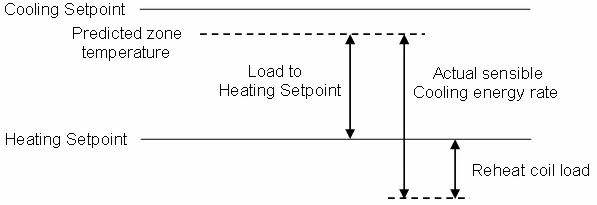
\includegraphics[width=0.9\textwidth, height=0.9\textheight, keepaspectratio=true]{media/image5145.png}
\caption{Supplemental heating coil load when predicted zone air temperature is above the heating Setpoint \protect \label{fig:supplemental-heating-coil-load-when-predicted-002}}
\end{figure}

If a heating load exists (Figure~\ref{fig:supplemental-heating-coil-load-when-predicted-003}), the supplemental heating coil is used to meet the heating coil load and at the same time offset the entire sensible cooling energy rate of the DX cooling coil (to meet the humidistat setpoint). Note that when a heating load exists and high humidity control is required, the heat pump operates at the user-specified cooling air flow rate for the entire simulation time step. As with the fan, and DX cooling coil, report variables associated with supplemental heating coil performance (e.g., heating coil energy, heating coil rate, heating coil gas or electric energy, heating coil runtime fraction, etc.) are managed in the supplemental (heating) coil object.

\begin{figure}[hbtp] % fig 229
\centering
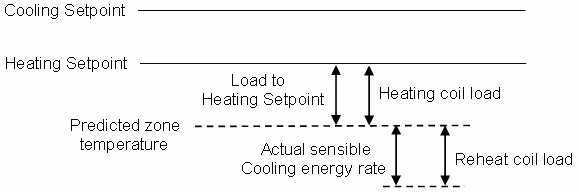
\includegraphics[width=0.9\textwidth, height=0.9\textheight, keepaspectratio=true]{media/image5146.png}
\caption{Supplemental heating coil load when predicted zone air temperature is below the heating setpoint \protect \label{fig:supplemental-heating-coil-load-when-predicted-003}}
\end{figure}

\subsection{Unitary Multi-Speed Air-To-Air Heat Pump}\label{unitary-multi-speed-air-to-air-heat-pump}

\subsubsection{Overview}\label{overview-4}

The input object AirLoopHVAC:UnitaryHeatPump:AirToAir:MultiSpeed provides a model for a multispeed air-to-air heat pump that is a ``virtual'' component that consists of an on/off or constant volume fan component, a multispeed DX cooling coil, a multispeed DX heating coil, and a gas or electric supplemental heating coil. The main difference between this heat pump object and other EnergyPlus heat pump objects is that this object allows from two to four discrete compressor speeds for heating and cooling operation (instead of a single speed for each mode). The specific configuration of the blow through heat pump is shown in the following figure. For a draw through heat pump, the fan is located between the DX heating coil and the supplemental heating coil.

\begin{figure}[hbtp] % fig 230
\centering
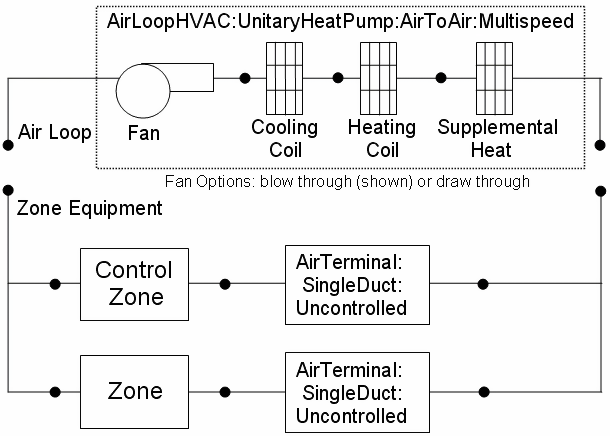
\includegraphics[width=0.9\textwidth, height=0.9\textheight, keepaspectratio=true]{media/image5147.png}
\caption{Schematic of a Multispeed Air-to-Air Heat Pump (Blow-through Configuration) \protect \label{fig:schematic-of-a-multispeed-air-to-air-heat}}
\end{figure}

While the heat pump may be configured to serve multiple zones, system operation is controlled by a thermostat located in a single ``control'' zone. One of the key parameters for the heat pump component is the fraction of the total system airflow that goes through the control zone. This fraction is calculated as the ratio of the maximum air mass flow rate for the air loop's supply inlet node for the control zone (e.g., AirTerminal:SingleDuct:ConstantVolume:NoReheat, field = Maximum Air Flow Rate, converted to mass flow) to the sum of the maximum air mass flow rates for the air loop's supply inlet nodes for all zones served by this air loop. The heat pump module scales the calculated load for the control zone upward based on this fraction to determine the total load to be met by the heat pump. The module then proceeds to calculate the required cycling ratio, speed ratio and speed number for the system coil and determines the supply air mass flow rate to meet this total load based on the speed number. The cycling ratio is the ratio of the sensible load (heating or cooling) to the steady-state capacity of the multispeed heat pump's DX heating or cooling coil at Speed 1 for the entire system time step. It is equivalent to the part load ratio for a single speed DX coil. The value is between 0.0 and 1.0 when the system operates at its lowest speed (Speed 1) and 1.0 when the multispeed heat pump operates at speeds above 1. The speed ratio is the ratio of time in a system time step that the compressor is at rated speed between two consecutive speed numbers ({[}Compressor Speed - Compressor speed at Speed i-1{]} / {[}Compressor speed at Speed i - Compressor speed at Speed i-1{]}). The compressor speed ratio is between 0.0 and 1.0 when the speed number is above 1 and is 0.0 during Speed 1 operation. The speed number is the lowest index number whose corresponding full-load sensible capacity at the given air mass flow rate is greater than or equal to the sensible load (heating or cooling) in a system time step. The heating or cooling capacity delivered by the heat pump is distributed to all of the zones served by this system via the direct air units that supply air to each zone.

The heat pump component is able to model supply air fan operation in two modes: cycling fan -- cycling coil (i.e., AUTO fan) and continuous fan -- cycling coil (i.e., fan ON). Fan:OnOff must be used to model AUTO fan, while Fan:OnOff or Fan:ConstantVolume can be used to model fan ON. The fan operation mode is specified using a supply air fan operating mode schedule where schedule values of 0 denote cycling fan operation and schedule values other than 0 (a 1 is usually used) denote continuous fan operation. Using this schedule, the supply air fan may be cycled with cooling or heating coil operation or operated continuously based on time of day (e.g.~cycling fan operation at night and continuous fan operation during the day).

Several output variables are reported by the heat pump object including fan part-load ratio, compressor part-load ratio, cycling ratio, speed ratio and speed number. Fan part-load ratio is defined as the actual air mass flow rate through the system for the time step divided by the operating supply air mass flow rate specified for the heat pump (\({{{{\dot m}_{actual}}} \mathord{\left/ {\vphantom {{{{\dot m}_{actual}}} {{{\dot m}_{design}}}}} \right. } {{{\dot m}_{ON}}}}\) ) at speed 1. Fan part-load ratio is set to 1.0 when the heat pump operates at speeds above 1. The operating supply air mass flow rate may be different for cooling, heating, and when no cooling or heating is required. Compressor part-load ratio is the actual load for the time step divided by the full-load sensible capacity (see Equation~\ref{eq:UnitaryMultiSpeedCyclingRatioCooling} or~\ref{eq:UnitaryMultiSpeedCyclingRatioHeating}). If the defrost strategy is reverse cycle for a DX heating coil, the compressor part-load ratio is the sum of the actual load and the defrost load divided by the full-load sensible capacity. Therefore, the compressor part load ratio for the DX heating coil may be greater than the cycling ratio. This heat pump object also reports the sensible, latent and total cooling and heating rate, as well as the electricity consumption for the unit with separate accounting of auxiliary electric consumption. Furthermore, five report variables related to waste heat recovery are available if the user chooses to model this option.

\subsubsection{Model Description}\label{model-description-4}

As described previously, the heat pump is a ``virtual'' component consisting of a fan, multispeed DX cooling coil, multispeed DX heating coil and supplemental heating coil. The sole purpose of the heat pump model is to properly coordinate the operation of the various system components. The following sections describe the flow of information within the model, as well as the differences between cycling and continuous supply air fan operation.

\subsubsection{Cooling Operation}\label{cooling-operation-2}

The description of heat pump cooling operation is divided in two sections: sensible capacity and average supply air flow rate. Actually, the determinations of capacity and supply air flow rate are related, so these calculations are performed in unison.

\paragraph{Capacity calculation}\label{capacity-calculation}

If EnergyPlus determines that the heat pump must supply cooling to the control zone to meet the zone air temperature setpoint, then the heat pump model computes the total sensible cooling load (negative) to be delivered to the zones being served based on the control zone sensible cooling load and the fraction of the heat pump air flow that goes through the control zone.

\begin{equation}
Heat~Pump~Cooling~Load = \frac{{Control~Zone~Cooling~Load}}{{Control~Zone~Air~Flow~Fraction}}
\end{equation}

The model then calculates the heat pump's sensible cooling energy rate delivered to the zones being served when the system runs at full-load conditions at the highest speed and when the DX cooling coil is OFF. If the supply air fan cycles with the compressor, then the sensible cooling energy rate is zero when the cooling coil is OFF. However if the fan is scheduled to run continuously regardless of coil operation, then the sensible cooling energy rate will not be zero when the cooling coil is OFF. Calculating the sensible cooling energy rate involves modeling the supply air fan (and associated fan heat) and the multispeed DX cooling coil. The multispeed DX heating coil and the supplemental heating coil are also modeled, but only to pass the air properties and mass flow rate from their inlet nodes to their outlet nodes. For each of these cases (full load at highest cooling speed and DX cooling coil OFF), the sensible cooling energy rate delivered by the heat pump is calculated as follows:

\begin{equation}
FullCoolOutpu{t_{Highest~Speed}} = \left( {{{\dot m}_{HighestSpeed}}} \right){\left( {{h_{out,full~load}} - {h_{control~zone}}} \right)_{HRmin}} - {\Delta_{sen,HighestSpeed}}
\end{equation}

\begin{equation}
NoCoolOutput = \left( {{{\dot m}_{coil~off}}} \right){\left( {{h_{out,coil~off}} - {h_{control~zone}}} \right)_{HRmin}} - {\Delta_{sen,coil~off}}
\end{equation}

where:

\({\dot m}_{HighestSpeed}\) is the air mass flow rate through heat pump at the highest cooling speed (kg/s)

\(h_{out,full~load}\) is the enthalpy of air exiting the heat pump at full-load conditions (J/kg)

\(h_{control~zone}\) is the enthalpy of air leaving the control zone (where thermostat is located) (J/kg)

\(HR_{min}\) is the minimum humidity ratio of the heat pump exiting air or the air leaving the control zone (kg/kg)

\({\dot m}_{CoilOff}\) is the air mass flow rate through the heat pump with the cooling coil OFF (kg/s)

\(h_{out,coil~off}\) is the enthalpy of air exiting the heat pump with the cooling coil OFF (J/kg)

\(\Delta_{sen,full~load}\) is the sensible load difference between the system output node and the zone inlet node at full-load conditions.

\begin{equation}
\begin{split}
{\Delta_{sen,HighestSpeed}} = \frac{{{{\dot m}_{Zone~Inlet}}}}{Frac}{\left( {{h_{Out,full~load}} - {h_{Zone~Inlet}}} \right)_{HRmin}} \\
+ \left( {{{\dot m}_{HighestSpeed}} - \frac{{{{\dot m}_{Zone~Inlet}}}}{Frac}} \right){\left( {h_{Out,full~load} - {h_{Control~Zone}}} \right)_{HRmin}}
\end{split}
\end{equation}

where:

Frac is the control zone air fraction with respect to the system mass flow rate

\(\Delta_{sen,coil~off}\) is the sensible load difference between the system output node and the zone inlet node with the cooling coil OFF conditions.

\begin{equation}
\begin{split}
{\Delta_{sen,coil~off}} = \frac{{{{\dot m}_{Zone~Inlet}}}}{{Frac}}{\left( {{h_{Out,coil~off}} - {h_{Zone~Inlet}}} \right)_{HRmin}} \\ 
+ \left( {{{\dot m}_{coil~off}} - \frac{{{{\dot m}_{Zone~Inlet}}}}{{Frac}}} \right){\left( {{h_{Out,coil~off}} - {h_{Control~Zone}}} \right)_{HRmin}}
\end{split}
\end{equation}

If the heat pump's sensible cooling rate at the highest speed (full load, no cycling) is insufficient to meet the entire cooling load, the controlled zone conditions will not be met. The reported cycling rate and speed ratio are 1, and the speed number is set to the highest index number. If the total sensible cooling load to be met by the system is less than the sensible cooling rate at the highest speed, then the following steps are performed.

First, calculate the sensible cooling energy rate at Speed 1:

\begin{equation}
FullCoolOutpu{t_{Speed1}} = \left( {{{\dot m}_{Speed1}}} \right){\left( {{h_{out,full~load}} - {h_{control~zone}}} \right)_{HRmin}} - {\Delta_{sen,Speed1}}
\end{equation}

where:

\({{{\dot m}_{Speed1}}}\) is the air mass flow rate through heat pump at Speed 1 (kg/s)

\(\Delta_{sen,Speed1}\) is the sensible load difference between the system output node and the zone inlet node at full-load conditions at Speed 1.

\begin{equation}
\begin{array}{rl}
{\Delta_{sen,Speed1}} =& \frac{{{{\dot m}_{Zone~Inlet}}}}{{Frac}}{\left( {{h_{Out,full~load}} - {h_{Zone~Inlet}}} \right)_{HRmin}} \\
 & + \left( {{{\dot m}_{Speed1}} - \frac{{{{\dot m}_{Zone~Inlet}}}}{{Frac}}} \right){\left( {{h_{Out,full~load}} - {h_{Control~Zone}}} \right)_{HRmin}}
\end{array}
\end{equation}

Second, if the sensible cooling energy rate delivered by the heat pump at Speed 1 is greater or equal to the sensible load, the cycling ratio (part-load ratio) for the heat pump is estimated.

\begin{equation}
  \begin{array}{rl}
    CyclingRatio &= \frac{\left|\PB{HeatingCoilSensibleLoad}\right|}{FullHeatingCoilCapacity} \\
                 &= \max \PB{0.0, \frac{\left|\PB{HeatPumpHeatingLoad-AddedFanHeat}\right|}{\left|\PB{FullHeatOutput_{Speed1}-AddedFanHeat_{Speed1}}\right|} }
  \end{array}
\label{eq:UnitaryMultiSpeedCyclingRatioCooling}
\end{equation}

where:

AddedFanHeat is the generated supply air fan heat, which is a function of part load ratio and as internal component cooling load (W)

AddedFanHeat\(_{Speed1}\) is the generated supply air fan heat at Speed 1 for a part load ratio of 1 (W).

Since the part-load performance of the DX cooling coil is frequently non-linear,and the supply air fan heat varies based on cooling coil operation for the case of cycling fan/cycling coil (AUTO fan), the final part-load ratio for the cooling coil compressor and fan are determined through iterative calculations (successive modeling of the cooling coil and fan) until the heat pump's cooling output matches the cooling load to be met within the convergence tolerance. The convergence tolerance is fixed at 0.001 and is calculated based on the difference between the load to be met and the heat pump's cooling output divided by the load to be met.

\begin{equation}
  Tolerance \equiv \frac{HeatPumpCoolingLoad - HeatPumpOutput_{Cycling}}{HeatPumpCoolingLoad} \leq 0.001
\end{equation}

where HeatPumpOutput\(_{Cycling}\) is the heat pump delivered sensible capacity for Speed 1 operating at a specific cycling ratio (W).

\begin{equation}
HeatPumpOutpu{t_{cycling}} = {\dot m_{_{HeatPump}}}{\left( {{h_{out}} - {h_{Control~Zone}}} \right)_{HRmin}} - {\Delta_{cycling}}
\end{equation}

where:

\({\dot m_{HeatPump}}\) is the average air mass flow rate defined in the next section (kg/s)

h\(_{out}\) is the enthalpy of air exiting the heat pump at part load conditions (J/kg)

\(\Delta_{cycling}\) is the average sensible load difference between the system output node and the zone inlet node.

\begin{equation}
  \begin{array}{rl}
    \Delta_{cycling} &= \frac{\dot{m}_{Zone~Inlet}}{Frac} \PB{h_{Zone~Inlet}-h_{Control~Zone}} \\
                           &+ \PB{\dot{m}_{HeatPump} - \frac{\dot{m}_{Zone~Inlet}}{Frac}} \PB{h_{Out} - h_{Control~Zone}}
  \end{array}
\end{equation}

where \({{{\dot m}_{Zone~Inlet}}}\) is the air mass flow rate in the supply inlet node in the controlled zone (kg/s).

For this case where speed 1 operation was able to meet the required cooling load, the speed ratio is set to zero and speed number is equal to 1.

Finally, if the heat pump's cooling output at full load for Speed 1 is insufficient to meet the entire cooling load, the Cycling ratio is set equal to 1.0 (compressor and fan are not cycling). Then the cooling speed is increased and the delivered sensible capacity is calculated. If the full load sensible capacity at Speed n is greater than or equal to the sensible load, the speed ratio for the heat pump is estimated:

\begin{equation}
Speed~Ratio = \frac{{ABS(Heat~Pump~Cooling~Load - AddedFanHeat - Full~Cool~ Outpu{t_{Speedn-1}})}}{{ABS(Full~Cool~Outpu{t_{Speedn}} - Full~Cool~Outpu{t_{Speedn-1}})}} 
\end{equation}

Although a linear relationship is assumed by applying the speed ratio to obtain the effective capacity and mass flow rate between speed n and n-1, the outlet air node conditions are dependent on the combined outputs and may not be linear. In addition, the supply air fan heat varies with the speed ratio due to different supply mass flow rates between speed n and n-1 . Therefore, the final speed ratio for the cooling coil compressor and fan are determined through iterative calculations (successive modeling of the cooling coil and fan) until the heat pump's cooling output matches the cooling load to be met within the convergence tolerance. The convergence tolerance is fixed at 0.001 and is calculated based on the difference between the load to be met and the heat pump's cooling output divided by the load to be met.

\begin{equation}
Tolerance = 0.001 \ge \frac{{Heat~Pump~Cooling~Load - HeatPumpOutpu{t_{SpeedRatio}}}}{{Heat~Pump~Cooling~Load}}
\end{equation}

where HeatPumpOutput\(_{SpeedRatio}\) is the heat pump delivered sensible capacity between two consecutive speeds at a specific speed ratio (W).

\begin{equation}
\begin{array}{rl}
HeatPumpOutpu{t_{SpeedRatio}} & = (SpeedRatio)FullCoolOutpu{t_{Speedn}} \\
 & = (1 - SpeedRatio)FullCoolOutpu{t_{Speedn-1}} - AddedFanHea{t_{SpeedRatio}}
\end{array}
\end{equation}

where AddedFanHeat\(_{SpeedRatio}\) is the generated supply air fan heat at a specific speed ratio (W).

In this case, the reported cycling ratio is 1 and speed number is equal to n.

\paragraph{Air Mass Flow Rate Calculation}\label{air-mass-flow-rate-calculation-2}

\emph{\textbf{Speed 1 operation}}

If the heat pump has been specified with cycling fan/cycling coil (AUTO fan), then the heat pump's operating supply air mass flow rate is determined by the cycling ratio (PartLoadRatio) for Speed 1. The supply air mass flow rate is multiplied by the cycling ratio to determine the average air mass flow rate for the system simulation time step. The air conditions at nodes downstream of the cooling coils represent the full-load (steady-state) values when the coil is operating.

\begin{equation}
{\dot m_{HeatPump}} = (CyclingRatio){\dot m_{Speed1}}
\end{equation}

If the fan operates continuously (i.e., when the supply air fan operating mode schedule values are NOT equal to 0), the operating air mass flow rate through the heat pump is calculated as the average of the user-specified air flow rate when the heat pump cooling coil is ON at Speed 1 and the user-specified air flow rate when the heat pump cooling coil is OFF (user-specified supply air volumetric flow rates converted to dry air mass flow rates).

\begin{equation}
{\dot m_{HeatPump}} = (CyclingRatio){\dot m_{Speed1}} + (1.0 - CyclingRatio){\dot m_{CoilOff}}
\end{equation}

where:

\({\dot m_{HeatPump}}\) is the average air mass flow rate through heat pump (kg/s)

\({{{\dot m}_{Speed1}}}\) is the air mass flow rate through heat pump when cooling coil is ON at Speed 1 (kg/s)

\({{{\dot m}_{CoilOff}}}\) is the air mass flow rate through heat pump when no heating or cooling is needed (kg/s).

In this case, the air conditions at nodes downstream of the cooling coils are calculated as the average conditions over the simulation time step (i.e., the weighted average of full-load conditions when the coil is operating and inlet air conditions when the coil is OFF).

\paragraph{Higher Speed Operation}\label{higher-speed-operation-1}

When the heat pump operates at higher speeds to meet the required cooling load, the supply air mass flow rate is linearly interpolated between two consecutive speeds:

\begin{equation}
{\dot m_{HeatPump}} = (SpeedRatio){\dot m_{Speedn}} + (1.0 - SpeedRatio){\dot m_{Speedn-1}}
\end{equation}

where:

\({\dot m_{HeatPump}}\) is the average air mass flow rate through the heat pump for the time step (kg/s)

\({\dot m_{Speedn}}\) is the air mass flow rate through heat pump when cooling coil is ON at Speed n (kg/s)

\({\dot m_{Speedn-1}}\) is the air mass flow rate through heat pump when cooling coil is ON at Speed n-1 (kg/s).

For this case of higher speed operation, the air conditions at nodes downstream of the cooling coils are determined by the delivered cooling capacity and supply air mass flow rates between two consecutive speeds.

Although the above sections present the capacity and air mass flow rate calculation separately, they are dependent and change every iteration until convergence is reached for the time step being simulated.

\subsubsection{Heating Operation}\label{heating-operation-1}

The description of heat pump heating operation is divided in two sections: total (sensible) capacity and average supply air flow rate. Actually, the determinations of capacity and supply air flow rate are related, so these calculation are performed in unison.

\paragraph{Capacity calculation}\label{capacity-calculation-1}

If EnergyPlus determines that the heat pump must supply heating to the control zone to meet the zone air temperature setpoint, then the heat pump model computes the total sensible heating load (positive) to be delivered to the zones being served based on the control zone sensible heating load and the fraction of the heat pump air flow that goes through the control zone.

\begin{equation}
Heat~Pump~Heating~Load = \frac{{Control~Zone~Heating~Load}}{{Control~Zone~Air~Flow~Fraction}}
\end{equation}

The model then calculates the heat pump's sensible heating energy rate delivered to the zones being served when the system runs at full-load conditions at the highest speed and when the DX heating coil is OFF (without supplemental heater operation in either case). If the supply air fan cycles with the compressor, then the sensible heating energy rate is zero when the compressor is OFF. However if the fan is scheduled to run continuously regardless of coil operation, then the sensible heating energy rate will not be zero when the compressor is OFF. Calculating the sensible heating energy rate involves modeling the supply air fan (and associated fan heat), the DX cooling coil (simply to pass the air properties and mass flow rate from its inlet node to its outlet node), the DX heating coil, and the supplemental heating coil (simply to pass the air properties and mass flow rate from its inlet node to its outlet node). For each of these cases (full load and DX heating coil OFF, without supplemental heater operation in either case), the sensible heating energy rate delivered by the heat pump is calculated as follows:

\begin{equation}
FullHeatOutpu{t_{HighestSpeed}} = \left( {{{\dot m}_{HighestSpeed}}} \right){\left( {{h_{out,full~load}} - {h_{control~zone}}} \right)_{HRmin}} - {\Delta_{sen,HighestSpeed}}
\end{equation}

\begin{equation}
NoHeatOutput = \left( {{{\dot m}_{CoilOff}}} \right){\left( {{h_{out,coil~off}} - {h_{control~zone}}} \right)_{HRmin}} - {\Delta_{sen,coil~off}}
\end{equation}

where:

\({\dot m}_{HighestSpeed}\) is the air mass flow rate through heat pump at the highest heating speed (kg/s)

\(h_{out,\, full\, load}\) is the enthalpy of air exiting the heat pump at full-load conditions (J/kg)

\(h_{control~zone}\) is the enthalpy of air leaving the control zone (where thermostat is located) (J/kg)

\(HR_{min}\) are the enthalpies evaluated at a constant humidity ratio, the minimum humidity ratio of the heat pump exiting air or the air leaving the control zone

\({\dot m}_{CoilOff}\) is the air mass flow rate through the heat pump with the heating coil OFF (kg/s)

\(h_{out,coil~off}\) is the enthalpy of air exiting the heat pump with the heating coil OFF (J/kg)

\(\Delta_{sen,full~load}\) is the sensible load difference between the system output node and the zone inlet node at full-load conditions.

\begin{equation}
\begin{array}{rl}
{\Delta_{sen,HighestSpeed}} =& \frac{{{{\dot m}_{Zone~Inlet}}}}{{Frac}}{\left( {{h_{Out,full~load}} - {h_{Zone~Inlet}}} \right)_{HRmin}} \\
 & + \left( {{{\dot m}_{HighestSpeed}} - \frac{{{{\dot m}_{Zone~Inlet}}}}{{Frac}}} \right){\left( {h_{Out,full~load} - {h_{Control~Zone}}} \right)_{HRmin}}
\end{array}
\end{equation}

where:

Frac = Control zone air fraction with respect to the system mass flow rate

\(\Delta_{sen,coil\, off}\) = Sensible load difference between the system output node and the zone inlet node with the heating coil OFF conditions

\begin{equation}
\begin{array}{rl}
{\Delta_{sen,coil~off}} =& \frac{{{{\dot m}_{Zone~Inlet}}}}{{Frac}}{\left( {{h_{Out,coil~off}} - {h_{Zone~Inlet}}} \right)_{HRmin}} \\
 & + \left( {{{\dot m}_{coil~off}} - \frac{{{{\dot m}_{Zone~Inlet}}}}{{Frac}}} \right){\left( {{h_{Out,coil~off}} - {h_{Control~Zone}}} \right)_{HRmin}}
\end{array}
\end{equation}

If the heat pump's DX heating coil output full load at the highest speed is insufficient to meet the entire heating load, the remaining heating load is passed to the supplemental heating coil. If the heat pump model determines that the outdoor air temperature is below the minimum outdoor air temperature for compressor operation (specified by the user), the compressor is turned off and the entire heating load is passed to the supplemental gas or electric heating coil. The heat pump exiting air conditions and energy consumption are calculated and reported by the individual component models (fan, DX heating coil, and supplemental gas or electric heating coil).

If the total heating load to be met by the system is less than the sensible heating rate at the highest speed, then the following steps are performed.

First, calculate the sensible heating energy rate at Speed 1:

\begin{equation}
FullHeatOutpu{t_{Speed1}} = \left( {{{\dot m}_{Speed1}}} \right){\left( {{h_{out,full~load}} - {h_{control~zone}}} \right)_{HRmin}} - {\Delta_{sen,Speed1}}
\end{equation}

where:

\({{{\dot m}_{Speed1}}}\) is the air mass flow rate through heat pump at Speed 1 (kg/s)

\(\Delta_{sen,Speed1}\) is the sensible load difference between the system output node and the zone inlet node at full-load conditions at Speed 1.

\begin{equation}
\begin{array}{rl}
{\Delta_{sen,Speed1}} =& \frac{{{{\dot m}_{Zone~Inlet}}}}{{Frac}}{\left( {{h_{Out,full~load}} - {h_{Zone~Inlet}}} \right)_{HRmin}} \\
 & + \left( {{{\dot m}_{Speed1}} - \frac{{{{\dot m}_{Zone~Inlet}}}}{{Frac}}} \right){\left( {{h_{Out,full~load}} - {h_{Control~Zone}}} \right)_{HRmin}}
\end{array}
\end{equation}

Second, if the sensible heating energy rate delivered by the heat pump at Speed 1 is greater or equal to the sensible load, the cycling ratio (part-load ratio) for the heat pump is estimated.

\begin{equation}
  \begin{array}{rl}
    CyclingRatio &= \frac{\left|\PB{HeatingCoilSensibleLoad}\right|}{FullHeatingCoilCapacity} \\
                 &= \max \PB{0.0, \frac{\left|\PB{HeatPumpHeatingLoad-AddedFanHeat}\right|}{\left|\PB{FullHeatOutput_{Speed1}-AddedFanHeat_{Speed1}}\right|} }
  \end{array}
\label{eq:UnitaryMultiSpeedCyclingRatioHeating}
\end{equation}

where:

AddedFanHeat is the generated supply air fan heat, which is a function of part load ratio and as internal component heating load (W)

AddedFanHeat\(_{Speed1}\) is the generated supply air fan heat at Speed 1 for a part load ratio of 1 (W).

Since the part-load performance of the DX heating coil is frequently non-linear (Ref: Single-Speed Electric Heat Pump DX Air Heating Coil), and the supply air fan heat varies based on heating coil operation for the case of cycling fan/cycling coil (AUTO fan), the final part-load ratio for the heating coil compressor and fan are determined through iterative calculations (successive modeling of the heating coil and fan) until the heat pump's heating output matches the heating load to be met within the convergence tolerance. The convergence tolerance is fixed at 0.001 and is calculated based on the difference between the load to be met and the heat pump's heating output divided by the load to be met.

\begin{equation}
  Tolerance \equiv \frac{HeatPumpHeatingLoad - HeatPumpOutput_{Cycling}}{HeatPumpHeatingLoad} \leq 0.001
\end{equation}

where HeatPumpOutput\(_{Cycling}\) is the heat pump delivered sensible capacity for Speed 1 operating at a specific cycling ratio (W).

\begin{equation}
HeatPumpOutpu{t_{cycling}} = {\dot m_{_{HeatPump}}}{\left( {{h_{out}} - {h_{Control\;Zone}}} \right)_{HR\min }} - {\Delta_{cycling}}
\end{equation}

where:

\({\dot m_{HeatPump}}\) is the average air mass flow rate defined in the next section (kg/s)

\(h_{out}\) is the enthalpy of air exiting the heat pump at part load conditions (J/kg)

\(\Delta_{cycling}\) is the average sensible load difference between the system output node and the zone inlet node.

\begin{equation}
  \begin{array}{rl}
    \Delta_{cycling} &= \frac{\dot{m}_{Zone~Inlet}}{Frac} \PB{h_{Zone~Inlet} - h_{Control~Zone}} \\
                           &+ \PB{\dot{m}_{HeatPump} - \frac{\dot{m}_{Zone~Inlet}}{Frac}} \PB{h_{Out} - h_{Control~Zone}}
  \end{array}
\end{equation}

where \({{{\dot m}_{Zone~Inlet}}}\) is the air mass flow rate in the supply inlet node in the controlled zone (kg/s).

For this case where speed 1 operation was able to meet the required heating load, the speed ratio is set to zero and speed number is equal to 1.

Finally, if the heat pump's heating output at full load for Speed 1 is insufficient to meet the entire heating load, the Cycling ratio (PartLoadRatio) is set equal to 1.0 (compressor and fan are not cycling). Then the heating speed is increased and the delivered sensible capacity is calculated. If the full load sensible capacity at Speed n is greater than or equal to the sensible load, the speed ratio for the heat pump is estimated:

\begin{equation}
Speed~Ratio = \frac{{ABS(Heat~Pump~Heating~Load - AddedFanHeat - Full~Heat~Outpu{t_{Speedn-1}})}}{{ABS(Full~Heat~Outpu{t_{Speedn}} - Full~Heat~Outpu{t_{Speedn-1}})}}
\end{equation}

Although a linear relationship is assumed by applying the speed ratio to obtain the effective capacity and air mass flow rate between speed n and n-1, the outlet node conditions are dependent on the combined outputs and may not be linear. In addition, the supply air fan heat varies based on heating coil operation for the case of cycling fan/cycling coil (AUTO fan). Therefore, the final speed ratio for the heating coil compressor and fan are determined through iterative calculations (successive modeling of the heating coil and fan) until the heat pump's heating output matches the heating load to be met within the convergence tolerance. The convergence tolerance is fixed at 0.001 and is calculated based on the difference between the load to be met and the heat pump's heating output divided by the load to be met.

\begin{equation}
Tolerance = 0.001 \ge \frac{{Heat~Pump~Heating~Load - HeatPumpOutpu{t_{SpeedRatio}}}}{{Heat~Pump~Heating~Load}}
\end{equation}

where Heat~Pump~Output\(_{SpeedRatio}\) is the heat pump delivered sensible capacity between two consecutive speeds at a specific ratio (W).

\begin{equation}
\begin{array}{rl}
HeatPumpOutpu{t_{SpeedRatio}} &= (SpeedRatio)FullHeatOutpu{t_{Speedn}} \\
 &= (1 - SpeedRatio)FullHeatOutpu{t_{Speedn-1}} - AddedFanHea{t_{SpeedRatio}}
 \end{array}
\end{equation}

where AddedFanHeat\(_{SpeedRatio}\) is the generated supply air fan heat at a specific speed ratio (W).

In this case, the reported cycling ratio is 1 and speed number is equal to n.

\paragraph{Air Mass Flow Rate Calculation}\label{air-mass-flow-rate-calculation-3}

The air mass flow rate calculations during heating operation are the same as those described above for cooling operation.

\subsubsection{Fan Placement}\label{fan-placement}

Supply air fan placement impacts the iteration strategy. When the fan placement type is blow through, the air mass flow rate and coil part load factor (PLF) affect the fan outlet conditions. Since the fan is upstream of the coil components with this fan placement, the fan outlet conditions are calculated without knowing the next component's performance at the beginning of each iteration. DX coil performance is strongly dependent on the inlet conditions, so without correct inlet conditions the DX coil components may not be simulated correctly. Therefore, the heat pump components are called twice for each iteration when fan placement is `blow through'. The correct part load factor for the fan component is obtained after the first call, so that the more realistic fan outlet conditions are used to simulate the coil performance in the second call. This extra call to the heat pump components is not required for the draw through fan since the supply air fan is located downstream of the DX coils with this fan placement.

\subsubsection{Waste Heat Calculation}\label{waste-heat-calculation-1}

When the heat recovery is active (the value of the Design Heat Recovery Water Flow Rate field is greater than 0), the outlet node temperature of heat recovery is calculated based on the recoverable waste heat generated by its child objects (Coil:Cooling:DX:MultiSpeed and Coil:Heating:DX:MultiSpeed):

\begin{equation}
{T_{outlet}} = {T_{inlet}} + \frac{{{Q_{WasteHeat}}}}{{{C_p}{{\dot m}_{hr}}}}
\end{equation}

where:

T\(_{outlet}\) is the outlet node temperature of heat recovery (\(^{\circ}\)C)

T\(_{inlet}\) is the inlet node temperature of heat recovery (\(^{\circ}\)C)

Q\(_{WasteHeat}\) is the recoverable waste heat generated by its child objects (W)

C\(_{p}\) is the inlet node temperature of heat recovery (\(^{\circ}\)C)

\({{{\dot m}_{hr}}}\) is the mass flow rate of heat recovery (kg/s).

If the outlet node temperature is above the value of the Maximum Temp for Heat Recovery field, the outlet node temperature is reset to the value of Maximum Temp for Heat Recovery.

\subsection{DX Cooling Package}\label{dx-cooling-package}

\subsubsection{Overview}\label{overview-5}

The DX cooling package subsystem model provides a ``virtual'' component that consists of a DX air cooling coil component as shown in the figure below. The CoilSystem:Cooling:DX input object provides a container component that controls the associated DX cooling coil which is specified in a separate object. This coil can be specified anywhere in the air loop simulation and is controlled by the setpoint(s) on the control node. Optional dehumidification controls may also be specified. CoilSystem:Cooling:DX assumes continuous fan operation for any given time step, because it is not able to control cycling fan operation in the way that other AirLoopHVAC:Unitary* systems can.

This system does not need any plant specification and will provide the electric consumption necessary to operate the compressor and the condenser fan.

\begin{figure}[hbtp] % fig 231
\centering
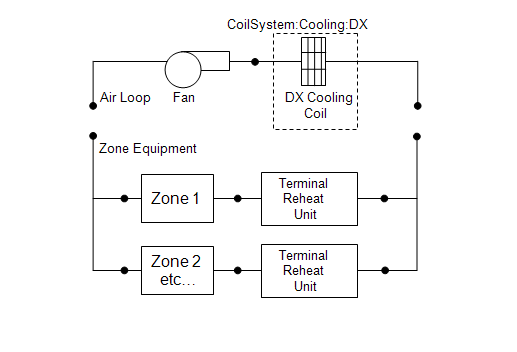
\includegraphics[width=0.9\textwidth, height=0.9\textheight, keepaspectratio=true]{media/image5198.png}
\caption{Schematic of Packaged DX Cooling Subsystem in Air Loop for a Blow-Thru Application \protect \label{fig:schematic-of-packaged-dx-cooling-subsystem-in}}
\end{figure}

\subsubsection{Controls}\label{controls-1}

The system calculates the current sensible load using the temperature of the inlet node and the System Node Setpoint Temp on the control node. If the control node is not the outlet node, the desired outlet node temperature is adjusted for the current temperature difference between the outlet node and the control node. Likewise, the current latent load is calculated using the humidity ratio of the inlet node and the System Node Humidity Ratio Max on the control node. The controls determine the required coil run-time fraction and dehumidification mode (if applicable) using the steps outlined below.

\paragraph{Step 1 -- Meet Sensible Load Requirement}\label{step-1-meet-sensible-load-requirement-1}

The controls first attempt to meet the sensible requirement. The specified DX coil model is called with a part-load ratio (PLR) of 1.0 to determine the full-load output of the coil. This is compared with the desired outlet node temperature and a sensible PLR is calculated. If the PLR is \textless{}1.0, a root solver iteration routine is called to determine the coil run-time fraction which results in the desired outlet node temperature. For a variable-speed DX cooling coil, if the load is smaller than the sensible capacity at the lowest speed, the coil run-time fraction is determined in the same way as a single-speed DX cooling coil. Otherwise, its speed level and speed ratio between two neighboring speeds are selected to match the load.

If the cooling coil type is specified as CoilSystem:Cooling:DX:CoolingHeatExchanganerAssisted and the dehumidification control type is specified as CoolReheat, the heat exchanger is active during this attempt to meet the sensible requirement.

\paragraph{Step 2 -- Meet Latent Load Requirement (if activated)}\label{step-2-meet-latent-load-requirement-if-activated-1}

If dehumidification controls are active, the leaving humidity ratio resulting from operation to meet the sensible load (Step 1 above) is compared with the desired outlet node humidity ratio. If the humidity requirement is already met, then no further control action is taken. If the humidity requirement has not been met, then the coil is re-simulated depending on the type of humidity control.

\paragraph{Step 2a -- Humidity Control = MultiMode}\label{step-2a-humidity-control-multimode-1}

If the humidity control type is MultiMode, then the coil's enhanced dehumidification mode is activated when the coil type is Coil:Cooling:DX:TwoStageWithHumidityControlMode or the heat exchanger is activated when the coil type is \\
CoilSystem:Cooling:DX:CoolingHeatExchangerAssisted and Step 1 above is repeated to meet the sensible load using the coil performance resulting from the enhanced dehumidification mode. This is a semi-passive approach to dehumidification which may fall short or may exceed the dehumidification requirement. If the user has specified Run on Latent Load = Yes in the CoilSystem:Cooling:DX object, and there is no sensible load to be met, then the system will try to meet the entire dehumidification load. If dehumidification mode should not be active when there is no sensible load, then choose Run on Latent Load = No.

\paragraph{Step 2b -- Humidity Control = CoolReheat}\label{step-2b-humidity-control-coolreheat-1}

If the humidity control type is CoolReheat, the coil is re-simulated to achieve the desired outlet node humidity ratio. This option is valid for all cooling coil types. When the coil type is Coil:Cooling:DX:TwoStageWithHumidityControlMode, only the cooling performance mode is used for this step and enhanced dehumidification mode is not activated.

\subsection{DX Heating Package}\label{dx-heating-package}

\subsubsection{Overview}\label{overview-6}

The DX heating package subsystem model provides a ``virtual'' component that consists of a DX air-to-air heating coil component and associated controls. The CoilSystem:Heating:DX input object provides a container component that controls the associated DX heating coil~ which is specified in a separate object. See the entry called Single-Speed and Variable-Speed Electric Heat Pump DX Air Heating Coil for details of the coil model itself.~ This coil can be specified anywhere in the air loop simulation and is controlled by the setpoint on the heating coil's outlet node. This model is analogous to the model for CoilSystem:Cooling:DX which is similar but for cooling.~ The model assumes continuous fan operation for any given time step, because it is not able to control cycling fan operation in the way that other AirLoopHVAC:Unitary* systems can.

This system does not need any plant specification and will provide the electric consumption necessary to operate the compressor and the condenser fan.

\subsubsection{Controls}\label{controls-2}

The DX heating package system calculates how the coil should operate to meet current sensible load using the temperature of the inlet node and the System Node Setpoint Temp on the outlet node. The controls determine the required coil run-time fraction to meet the sensible requirement. The Single-Speed Electric Heat Pump DX Air Heating Coil model is called with a part-load ratio (PLR) of 1.0 to determine the full-load output of the coil. If the PLR is \textless{}1.0, a root solver iteration routine is called to determine the coil run-time fraction which results in the desired outlet node temperature. For a variable-speed DX heating coil, if the load is smaller than the heating capacity at the lowest speed, the coil run-time fraction is determined in the same way as a single-speed DX heating coil. Otherwise, its speed level and speed ratio between two neighboring speeds are selected to match the load.

\subsection{Desiccant Dehumidifier Package}\label{desiccant-dehumidifier-package}

\subsubsection{Overview}\label{overview-7}

The input object Dehumidifier:Desiccant:System provides a model that packages components for a desiccant-based subsystem that dehumidifies an air stream, normally called the process air stream. A second heated air stream, called the regeneration air stream, is used to remove the collected moisture from the desiccant heat exchanger and this moisture-laden air is then usually exhausted from the building. This Dehumidifier:Desiccant:System object is similar to the Dehumidifier:Desiccant:NoFans object but has some additional modeling capabilities.

The Dehumidifier:Desiccant:System desiccant dehumidifier object in EnergyPlus is a compound object that can be placed anywhere in an air loop. Common locations for this object are in an AirLoopHVAC:OutdoorAirSystem or in the main air loop downstream of a cooling coil (postcooling desiccant dehumidifier). This compound object coordinates the operation of several `children' objects: a desiccant heat exchanger, a regeneration air fan, and an optional regeneration air heater. If this dehumidifier is placed in the main air loop immediately downstream of a direct expansion (DX) cooling coil, then the dehumidifier's operation can be coordinated with the operation of the companion DX coil and it is also possible to specify that the DX system's condenser waste heat can be used to help regenerate the desiccant heat exchanger. For the case of condenser waste heat regeneration, an optional exhaust fan can also be modeled by this desiccant dehumidifier compound object to help maintain a setpoint temperature for air entering the regeneration side of the desiccant heat exchanger. Refer to the EnergyPlus Input Output Reference for the specific input syntax for this desiccant dehumidifier object.

\begin{figure}[hbtp] % fig 232
\centering
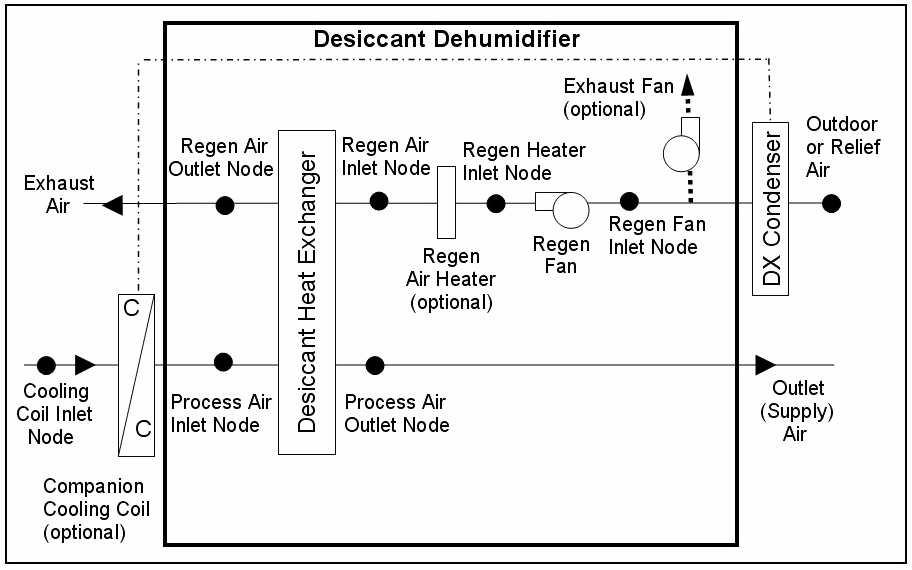
\includegraphics[width=0.9\textwidth, height=0.9\textheight, keepaspectratio=true]{media/image5199.png}
\caption{Schematic of a Desiccant Dehumidifier with Draw Through Regeneration Fan Placement \protect \label{fig:schematic-of-a-desiccant-dehumidifier-with}}
\end{figure}

\begin{figure}[hbtp] % fig 233
\centering
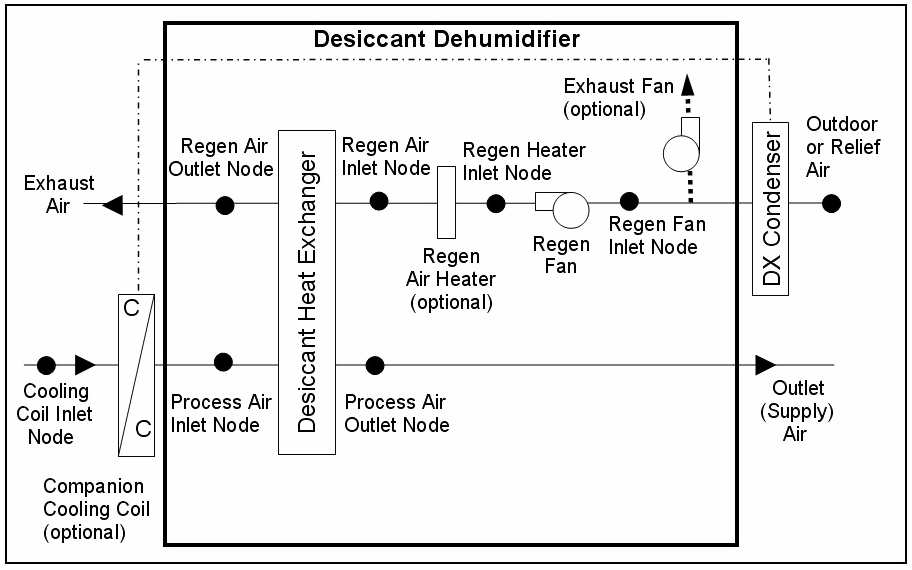
\includegraphics[width=0.9\textwidth, height=0.9\textheight, keepaspectratio=true]{media/image5200.png}
\caption{Schematic of a Desiccant Dehumidifier in Blow Through Regeneration Fan Placement \protect \label{fig:schematic-of-a-desiccant-dehumidifier-in-blow}}
\end{figure}

\subsubsection{Control Logic}\label{control-logic}

The model first decides if the dehumidifier can operate for the simulation time step, based on its availability schedule and if there is air flow detected on the process air inlet node. If available to operate, then the target humidity ratio for the process outlet air is determined based on the maximum humidity ratio setpoint on the control node (System Node Setpoint Humidity Ratio Max). If the control node is not the process air outlet node, the target humidity ratio is adjusted for the current humidity ratio difference between the process air outlet node and the control node. If the humidity ratio of the process inlet air is greater than the target humidity ratio for the process outlet air, then the dehumidifier operates to meet the target to the extent possible.

Once it is determined that the dehumidifier should operate, the components upstream of the desiccant heat exchanger's regeneration inlet are modeled. The actual components that are modeled depend on the configuration specified by the user.

If the waste heat from the companion cooling coil is being used to heat the regeneration air, then this model determines the temperature of the air leaving the cooling coil condenser. The user may also specify a setpoint temperature for the regeneration air entering the desiccant heat exchanger and an optional exhaust fan, which can impact the condenser leaving air temperature. For this case, the exhaust fan is used to control the condenser leaving air temperature by boosting the air flow rate through the condenser to meet the setpoint temperature (minus regeneration fan heat if blow through fan placement).

Note: If the desiccant dehumidifier is OFF for a simulation time step but its companion cooling coil is operating and is specified to provide regeneration air heating, then the exhaust fan operates at the maximum air flow rate (i.e., this fan serves at the condenser fan for the companion cooling coil system when regeneration air heating is specified, so the inputs for the companion cooling coil object should not include the condenser fan energy since the condenser fan energy is modeled by the Dehumidifier:Desiccant:SystemDesiccant Dehumidifier object).

The exhaust fan power is determined as follows:

If dehumidifier is operating:

\begin{equation}
  \begin{array}{rl}
    PLR_{exhaust} &= \frac{\dot{m}_{exhaust}}{\rho_{Std}\dot{V}_{exhaust,max}} \\
    P_{exhaust} &= P_{exhaust,max} \times ExhFanModFac
  \end{array}
\end{equation}

If dehumidifier is not operating, but companion coil is operating:

\begin{equation}
  P_{exhaust} = P_{exhaust,max} \times PLR_{companion~coil}
\end{equation}

where:

\(PL{R_{exhaust}}\) is the part load ratio of the exhaust fan

\({\dot{V}_{exhaust,max}}\) is the exhaust fan maximum volumetric flow rate, user input (m\(^{3}\)/s)

\({\rho_{Std}}\) is the density of air at standard temperature and pressure {[}dry air at 20$^\circ$C{]} (m\(^{3}\)/kg)

\({P_{exhaust,max}}\) is the exhaust fan maximum power, user input (W)

\(ExhFanModFac\) is the exhaust fan power modifier curve evaluated at PLR\(_{exhaust}\). If modifier curve not provided by the user, then this factor is assumed to be 1.0.

\(PL{R_{companion~coil}}\) is the part load ratio of the companion cooling coil

\({P_{exhaust}}\) is the output variable `Dehumidifier Exhaust Fan Electric Power, W'.

The exhaust fan electric consumption is then calculated as:

\begin{equation}
{E_{exhaust}} = {P_{exhaust}}*TimeStepSys*3600
\end{equation}

where:

\({E_{exhaust}}\) is the output variable `Dehumidifier Exhaust Fan Electric Energy, J'

\(TimeStepSys\) is the HVAC system simulation time step (hr).

Once the outlet conditions from the companion coil condenser are determined (if present), then the regeneration air fan (if blow through configuration) and regeneration air heater (if present) are simulated. To the extent possible (e.g., if the heater is available to operate based on its availability schedule and it has sufficient heating capacity), the regeneration air heater operates to raise its outlet air temperature to the specified regeneration inlet air setpoint temperature.

With the inlet air conditions to the regeneration and process sides of the desiccant heat exchanger now known, the performance of the desiccant heat exchanger is modeled. If the desiccant dehumidifier is specified with a companion cooling coil upstream of the heat exchanger's process inlet, then the model assumes that the dehumidifier operates at the same time as the companion coil (same part-load ratio). If not, then the desiccant dehumidifier model calculates the fraction of time it must operate to meet the process outlet air maximum humidity target (setpoint) using the following equation:

\begin{equation}
  \begin{array}{rl}
    DDPartLoadRatio &= \frac{w_{Proc,in} - w_{max,setpoint}}{w_{Proc,in} - w_{Proc,out,HXon}} \\
    DDPartLoadRatio &= \max\PB{0.0,DDPartLoadRatio} \\
    DDPartLoadRatio &= \min\PB{1.0,DDPartLoadRatio}
  \end{array}
\end{equation}

where:

\(\,DDPartLoadRatio\) is the output variable `Dehumidifier Part Load Ratio'

\({w_{Proc,in}}\) is the process inlet air humidity ratio (kg/kg)

\({w_{max,setpoint}}\) is the target humidity ratio (setpoint) for the process outlet air (kg/kg)

\({w_{Proc,out,HXon}}\) is the process outlet air humidity ratio when the desiccant heat exchanger operates (kg/kg).

After all of the desiccant dehumidifier components are modeled at the appropriate part load ratio, the water removal rate and water removed are calculated.

\begin{equation}
  \begin{array}{rl}
    \dot{m}_{water~removed,Proc} & = \dot{m}_{Proc,in} \PB{w_{Proc,in} - w_{Proc,out}} \\
    m_{water~removed,Proc}       & = \dot{m}_{water~removed,Proc} \times TimeStepSys \times 3600
  \end{array}
\end{equation}

where:

\({\dot{m}_{water~removed,Proc}}\) is the output variable `Dehumidifier Removed Water Mass Flow Rate, kg/s'

\({\dot{m}_{Proc,in}}\) is the air mass flow rate at the process air inlet node (kg/s)

\({w_{Proc,out}}\) is the process outlet air humidity ratio (kg/kg)

\({m_{water~removed,Proc}}\) is the output variable `Dehumidifier Removed Water Mass, kg'.

\subsubsection{References}\label{references-000}

ASHRAE. 2004. Chapter 22: Desiccant Dehumidification and Pressure-Drying Equipment. 2004 ASHRAE HVAC Systems and Equipment Handbook. Atlanta, GA: American Society of Heating, Refrigerating and Air-Conditioning Engineers, Inc.

Kosar, D. 2006. Dehumidification Enhancements, ASHRAE Journal, Vol. 48, No. 2, February 2006.

Kosar, D. et al. 2006. Dehumidification Enhancement of Direct Expansion Systems Through Component Augmentation of the Cooling Coil. 15\(^{th}\) Symposium on Improving Building Systems in Hot and Humid Climates, July 24-26, 2006.

\subsection{Unitary Water-To-Air Heat Pump}\label{unitary-water-to-air-heat-pump}

\subsubsection{Overview}\label{overview-8}

The input object AirLoopHVAC:UnitaryHeatPump:WaterToAir provides a model for a water-to-Air heat pump that is a ``virtual'' component that consists of an on/off fan component, a water-to-air heat pump cooling coil, a water-to-air heat pump heating coil, and a gas or electric supplemental heating coil. The specific configuration of the blowthru heat pump is shown in the following figure. For a drawthru heat pump, the fan is located between the water-to-air heat pump heating coil and the supplemental heating coil. The configuration of the water-to-air heat pump in the air loop is similar to an air-to-air heat pump. In addition, a water-to-air heat pump has a water loop connection on its source side. The water loop can be served by a condenser loop (like GHE for Ground source systems), or by a cooling tower/ boiler plant loop (for water loop systems).

\begin{figure}[hbtp] % fig 234
\centering
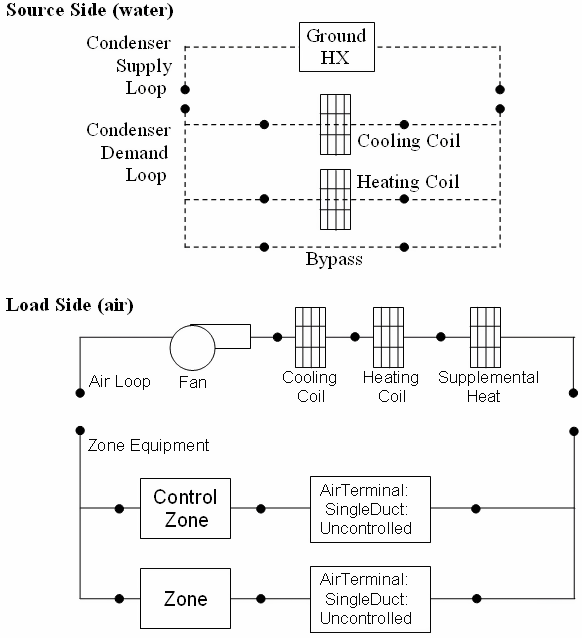
\includegraphics[width=0.9\textwidth, height=0.9\textheight, keepaspectratio=true]{media/image5222.png}
\caption{Source Side and Load Side Configuration of a BlowThru Water-To-Air Heat Pump \protect \label{fig:source-side-and-load-side-configuration-of-a}}
\end{figure}

There are two different models for water-to-air heat pump cooling and heating coils. Cooling and heating coils are modeled using a Single Speed or Variable Speed Equation Fit model or a Parameter Estimation model. The parameter estimation procedure is quite detailed and the equation fit model is designed to simplify the user inputs. Each model is discussed in short in the following sections. The Variable-Speed Equation Fit model is described in a separate section, as Coil:Cooling:WaterToAirHeatPump:VariableSpeedEquationFit and Coil:Heating:WaterToAirHeatPump:VariableSpeedEquationFit.

\subsubsection{Single Speed Equation-Fit Model:}\label{single-speed-equation-fit-model}

This section describes the equation-fit model for Water-to-Air heat pump (Object names: \textbf{Coil:Cooling:WaterToAirHeatPump:EquationFit} and \\ \textbf{Coil:Heating:WaterToAirHeatPump:EquationFit}). This documentation is derived from the M.S. dissertation of Tang (2005) which is available on the Oklahoma State University web site . The model uses five non-dimensional equations or curves to predict the heat pump performance in cooling and heating mode. The methodology involved using the generalized least square method to generate a set of performance coefficients from the catalog data at indicated reference conditions. Then the respective coefficients and indicated reference conditions are used in the model to simulate the heat pump performance. The variables or inlet conditions that influenced the water-to-air heat pump performance are load side inlet water temperature, source side inlet temperature, source side water flow rate and load side water flow rate. The governing equations for the cooling and heating mode are as following:

Cooling Mode:

\begin{equation}
\frac{{Q{}_{total}}}{{Q{}_{total,ref}}} = A1 + A2\left[ {\frac{{{T_{wb}}}}{{{T_{ref}}}}} \right] + A3\left[ {\frac{{T{}_{w,in}}}{{T{}_{ref}}}} \right] + A4\left[ {\frac{{{{\dot V}_{air}}}}{{{{\dot V}_{air,ref}}}}} \right] + A5\left[ {\frac{{{{\dot V}_w}}}{{{{\dot V}_{w,ref}}}}} \right]
\end{equation}

\begin{equation}
\frac{{{Q_{sens}}}}{{{Q_{sens,ref}}}} = B1 + B2\left[ {\frac{{T{}_{db}}}{{T{}_{ref}}}} \right] + B3\left[ {\frac{{T{}_{wb}}}{{T{}_{ref}}}} \right] + B4\left[ {\frac{{T{}_{w,in}}}{{T{}_{ref}}}} \right] + B5\left[ {\frac{{{{\dot V}_{air}}}}{{{{\dot V}_{air,ref}}}}} \right] + B6\left[ {\frac{{\dot V{}_w}}{{\dot V{}_{w,ref}}}} \right]
\end{equation}

\begin{equation}
\frac{{Power{}_c}}{{Power{}_{c,ref}}} = C1 + C2\left[ {\frac{{{T_{wb}}}}{{{T_{ref}}}}} \right] + C3\left[ {\frac{{T{}_{w,in}}}{{T{}_{ref}}}} \right] + C4\left[ {\frac{{{{\dot V}_{air}}}}{{{{\dot V}_{air,ref}}}}} \right] + C5\left[ {\frac{{{{\dot V}_w}}}{{{{\dot V}_{w,ref}}}}} \right]
\end{equation}

Heating Mode:

\begin{equation}
\frac{{{Q_h}}}{{Q{}_{h,ref}}} = E1 + E2\left[ {\frac{{{T_{db}}}}{{{T_{ref}}}}} \right] + E3\left[ {\frac{{T{}_{w,in}}}{{T{}_{ref}}}} \right] + E4\left[ {\frac{{{{\dot V}_{air}}}}{{{{\dot V}_{air,ref}}}}} \right] + E5\left[ {\frac{{{{\dot V}_w}}}{{{{\dot V}_{w,ref}}}}} \right]
\end{equation}

\begin{equation}
\frac{{Power{_h}}}{{Power{}_{h,ref}}} = F1 + F2\left[ {\frac{{{T_{db}}}}{{{T_{ref}}}}} \right] + F3\left[ {\frac{{T{}_{w,in}}}{{T{}_{ref}}}} \right] + F4\left[ {\frac{{{{\dot V}_{air}}}}{{{{\dot V}_{air,ref}}}}} \right] + F5\left[ {\frac{{{{\dot V}_w}}}{{{{\dot V}_{w,ref}}}}} \right]
\end{equation}

Assuming no losses, the source side heat transfer rate for cooling and heating mode is calculated as following:

\begin{equation}
{Q_{source,c}} = {Q_{total}} + Powe{r_c}
\end{equation}

\begin{equation}
{Q_{source,h}} = {Q_h} - Powe{r_h}
\end{equation}

where:

\(A1 - F5\) are the equation fit coefficients for the cooling and heating mode

\({T_{ref}}\) is 283K

\({T_{w,in}}\) is the entering water temperature (K)

\({T_{db}}\) is the entering air dry-bulb temperature (K)

\({T_{wb}}\) is the entering air wet-bulb temperature (K)

\({\dot V_{air}}\) is the load side air volumetric flow rate (m\(^{3}\)/s)

\({\dot V_w}\) is the source side water volumetric flow rate (m\(^{3}\)/s)

\({Q_{total}}\) is the total cooling capacity (W)

\({Q_{sens}}\) is the sensible cooling capacity (W)

\(Powe{r_c}\) is the power consumption in cooling mode (W)

\({Q_{source,c}}\) is the source side heat transfer rate in cooling mode (W)

\({Q_h}\) is the total heating capacity (W)

\(Powe{r_h}\) is the power consumption in heating mode (W)

\({Q_{source,h}}\) is the source side heat transfer rate in heating mode (W).

The inlet conditions or variables are divided by the reference conditions. This formulation allows the coefficients to fall into smaller range of values. Moreover, the value of the coefficient indirectly represents the sensitivity of the output to that particular inlet variable. The reference conditions used when generating the performance coefficients must be the same as the reference conditions used later in the model. The reference temperature \({T_{ref}}\) is fixed at 283K. Temperature unit of Kelvin is used instead of Celsius to keep the ratio of the water inlet temperature and reference temperature positive value should the water inlet temperature drop below the freezing point.

For cooling mode, the reference conditions; reference load side air volumetric flow rate \(\left( {{{\dot V}_{air,ref}}} \right)\), reference source side water volumetric flow rate\(\left( {{{\dot V}_{w,ref}}} \right)\), reference sensible capacity \(\left( {{Q_{sens,ref}}} \right)\) and reference power input \(\left( {Powe{r_{c,ref}}} \right)\) are the conditions when the heat pump is operating at the highest cooling capacity or reference cooling capacity \(\left( {{Q_{total,ref}}} \right)\) indicated in the manufacturer's catalog. Note that the reference conditions for heating mode might differ from the reference conditions specified for the cooling mode.

\subsubsection{Coefficient estimation procedure:}\label{coefficient-estimation-procedure}

The generalized least square method is used to generate the coefficients. This method utilizes an optimization method which calculates the coefficients that will give the least amount of differences between the model outputs and the catalog data. A set of coefficients for the cooling mode is generated which includes A1-A5 for total cooling capacity, B1-B6 for sensible cooling capacity, and C1-C5 for power consumption. The same procedure is repeated for the heating mode to generate the coefficients E1-E5 and F1-F5. An information flow chart showing the inputs, reference conditions, performance coefficients and outputs are shown in the Figure~\ref{fig:information-flow-chart-for-water-to-air-heat}.

\begin{figure}[hbtp] % fig 235
\centering
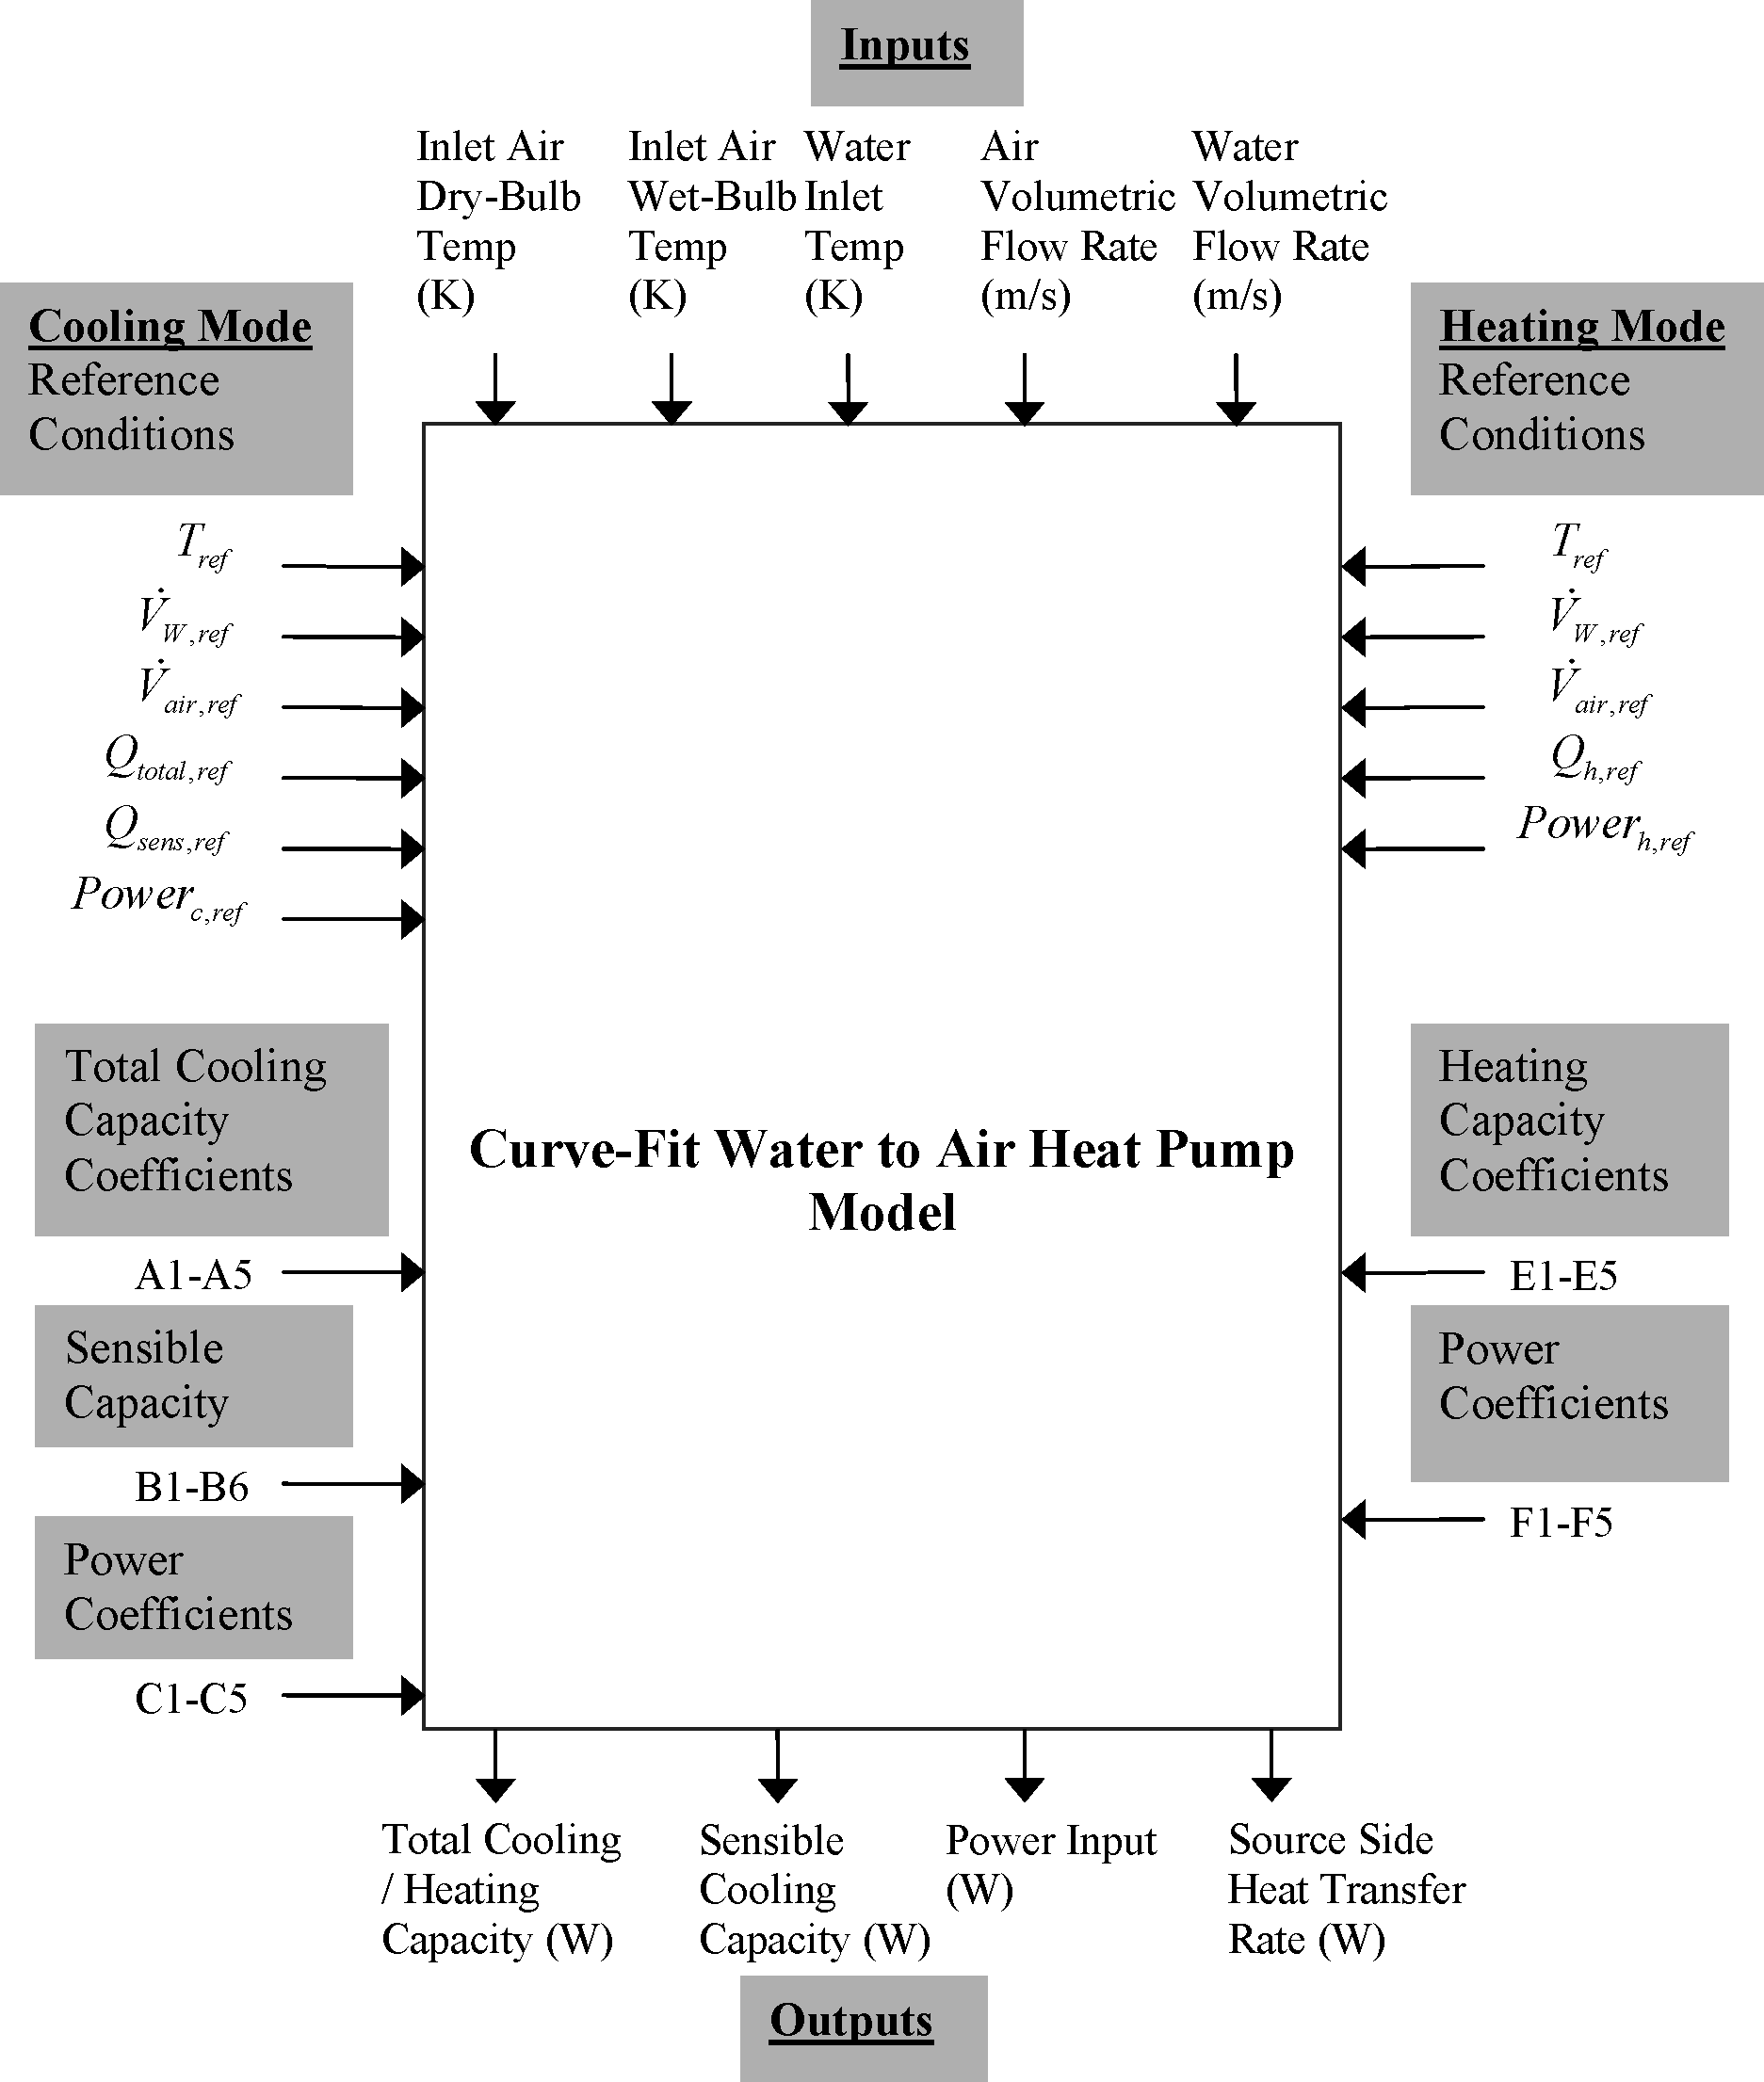
\includegraphics[width=0.9\textwidth, height=0.9\textheight, keepaspectratio=true]{media/image5250.png}
\caption{Information Flow Chart for Water-to-Air Heat Pump Equation Fit Model (Tang 2005) \protect \label{fig:information-flow-chart-for-water-to-air-heat}}
\end{figure}

\subsubsection{High Humidity Control with WaterToAir HeatPump Equation Fit model}\label{high-humidity-control-with-watertoair-heatpump-equation-fit-model}

The specific configuration of the WaterToAir HeatPump with supplemental heating coil is shown above (see Figure~\ref{fig:source-side-and-load-side-configuration-of-a}). This figure shows the fan placement when a blow through fan is specified. If a draw through fan is specified, the fan is located between the heating coil and the reheat coil. The system is controlled to keep the high relative humidity in the control zone from exceeding the setpoint specified in the object ZoneControl:Humidistat. When high humidity control is specified and the compressor operates, the heatpump always operates at the cooling air flow rate when a zone heating load is present as determined by the zone thermostat. High humidity control is specified as either None, or CoolReheat in the Dehumidification Control Type input field. CoolReheat is specified when a DX cooling coil is used to over-cool the supply air stream in order to meet the zone latent load. In this case, a supplemental heating coil will ensure the zone temperature does not fall below the zone heating temperature set point. If the dehumidification control type is selected as None, the WaterToAir HeatPump runs only to meet the sensible cooling load. A supplemental heating coil is required for all dehumidification control types.

The model first calculates the \emph{PartLoadRatio} required meeting the sensible cooling load.~ The heatpump's sensible cooling load is determined from the control zone sensible cooling load to the cooling setpoint and the control zone air flow fraction to maintain the dry-bulb temperature setpoint in the control zone:

\begin{equation}
HeatPumpCoolingLoad = \frac{{ControlZoneCoolingLoad}}{{ControlZoneAirFlowFraction}}
\end{equation}

The heatpump's sensible cooling load to be met and the full load cooling output are used to calculate the sensible the part-load ratio iteratively based on user specified convergence criterion.

\begin{equation}
PartLoadRatio = MAX\left( {0.0,\frac{{ABS\left( {HeatPumpCoolingLoad - NoCoolOutput} \right)}}{{ABS\left( {FullCoolOutput - NoCoolOutput} \right)}}} \right)
\end{equation}

When the heat pumps sensible cooling capacity meets the system sensible cooling load at a given sensible part load ratio, then the Heat pump meets the controlled zone cooling setpoint temperature.~ If a moisture (latent) load exists because the control zone humidity has exceeded the setpoint, the total moisture load to be met by the heat pumps (HeatPumpMoistureLoad) is calculated based on the control zone moisture load and the control zone air flow fraction.

\begin{equation}
HeatPumpMoistureLoad = \frac{{ControlZoneMoitureLoad}}{{ControlZoneAirFlowFraction}}
\end{equation}

Then the \emph{LatentPartLoadRatio} required to meet the high humidity setpoint is calculated as follows:

\begin{equation}
LatentPartLoadRatio = MIN\left( {PL{R_{Min}},\frac{{ABS\left( {HeatPumpMoistureLoad - NoLatentOutput} \right)}}{{ABS\left( {FullLatentOutput - NoLatentOutput} \right)}}} \right)
\end{equation}

The model uses the greater of the two part-load ratios, \emph{PartLoadRatio} or \emph{LatentPartLoadRatio}, to determine the operating part-load ratio of the Heat Pump's DX cooling coil.

\begin{equation}
LatentPartLoadRatio = MAX\left( {PartLoadRatio,LatentPartLoadRatio} \right)
\end{equation}

As previously described, iterations are performed to converge on the solution within the convergence tolerance.

where:

\(ControlZoneCoolingLoad\) is the control zone sensible cooling load to the cooling setpoint (W)

\(ControlZoneMoistureLoad\) is the control zone moisture load to the dehumidifying relative humidity setpoint (W)

\(ControlZoneAirFlowFraction\) ~~~~ =is  the supply air fraction that goes though the control zone

\emph{FullLatentOutput} is the Heat Pump's latent cooling energy rate at full-load conditions (W)

\emph{NoLatentOutput} is the Heat Pump's latent cooling energy rate with cooling coil OFF (W)

\(PartLoadRatio\) is the heat pump's part-load-ratio required to meet system sensible load

\(LatentPartLoadRatio\) is the heat pump's part-load-ratio required to meet system moisture load

\(PL{R_{MIN}}\) is the minimum part-load ratio, which is usually 0.0. For the case when the latent capacity degradation model is used (Ref: DX Cooling Coil Model), this value is the minimum part-load ratio at which the cooling coil will dehumidify the air.

When the predicted zone air temperature is above the heating setpoint and if there is a dehumidification load, the supplemental heating coil load is required to offset the excess cooling as shown in Figure~\ref{fig:supplemental-heating-coil-load-when-predicted-004}. If the model determines that the LatentPartLoadRatio is to be used as the operating part-load ratio of the heatpump's cooling coil, the supplemental coil is used to offset the excess sensible capacity provided by the unit. The model first checks the sensible load that exists for the current simulation time step (predicted zone temperature with no HVAC operation compared to the thermostat setpoint temperatures). If a sensible cooling load or no sensible cooling or heating load exists (see Figure~\ref{fig:supplemental-heating-coil-load-when-predicted-004}),~ the model calculates the difference between the sensible heating load required to reach or maintain the heating dry-bulb temperature setpoint and the actual sensible cooling energy rate delivered by the heat pump (with LatentPartLoadRatio). In this case, the supplemental heating coil is used to offset the excess sensible cooling energy provided by the DX cooling coil (if any) that could have caused an overshoot of the heating dry-bulb temperature setpoint. Note that when a humidistat is used and high humidity control is required, the zone dry-bulb temperature will typically move toward the heating temperature setpoint when a high moisture (latent) load exists.

\begin{figure}[hbtp] % fig 236
\centering
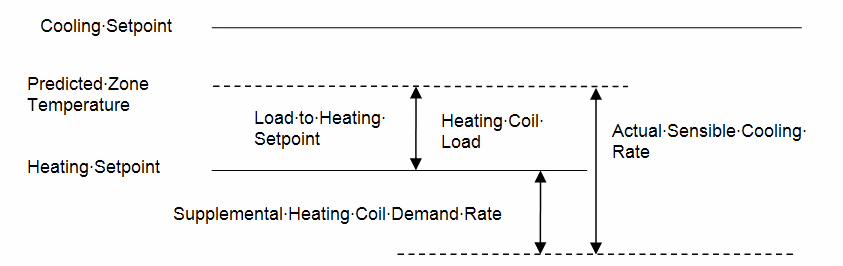
\includegraphics[width=0.9\textwidth, height=0.9\textheight, keepaspectratio=true]{media/image5262.png}
\caption{Supplemental heating coil load when predicted zone air temperature is above the heating Setpoint \protect \label{fig:supplemental-heating-coil-load-when-predicted-004}}
\end{figure}

If a heating load exists (Figure~\ref{fig:supplemental-heating-coil-load-when-predicted-005}), the supplemental heating coil is used to meet the heating coil load and at the same time offset the entire sensible cooling energy rate of the DX cooling coil (to meet the humidistat setpoint). Note that when a heating load exists and high humidity control is required, the heat pump operates at the user-specified cooling air flow rate for the entire simulation time step. As with the fan, and DX cooling coil, report variables associated with supplemental heating coil performance (e.g., heating coil energy, heating coil rate, heating coil gas or electric energy, heating coil runtime fraction, etc.) are managed in the supplemental (heating) coil object.

\begin{figure}[hbtp] % fig 237
\centering
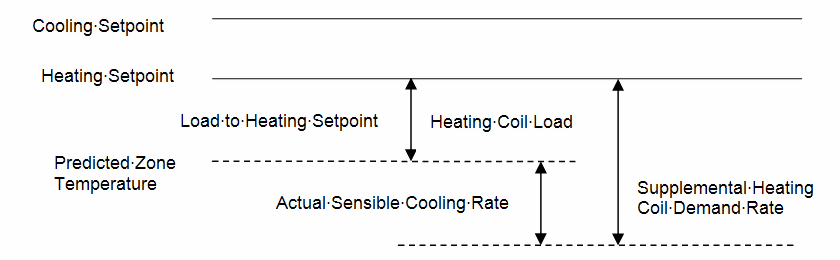
\includegraphics[width=0.9\textwidth, height=0.9\textheight, keepaspectratio=true]{media/image5263.png}
\caption{Supplemental heating coil load when predicted zone air temperature is below the heating setpoint \protect \label{fig:supplemental-heating-coil-load-when-predicted-005}}
\end{figure}

\subsubsection{Parameter Estimation Model}\label{parameter-estimation-model}

The steady state simulation model (Object: AirLoopHVAC:UnitaryHeatPump:WaterToAir) for a water-to-air vapor compression heat pump is described in this section. The model is implemented under the air-loop manager similar to the algorithm discussed under AirLoopHVAC:UnitaryHeatPump. The heat pump `coil' objects \\
(Coil:Cooling:WaterToAirHeatPump:ParameterEstimation and Coil:Heating:WaterToAirHeatPump:ParameterEstimation) actually consist of a steady state simulation of the unitary heat pump in cooling or heating mode respectively.~ This documentation is derived from the Ph.D.~dissertation of Hui Jin which is available on the Oklahoma State University web site . ~The model parameters, solution technique and solution algorithm are all identical to that of the water to water heat pump.~ The only difference between the two models is in the modeling of the water to air heat exchanger.

The effectiveness of this heat exchanger is given by:

\begin{equation}
\varepsilon  = 1 - {e^{ - NTU}}
\end{equation}

where NTU is defined by:

\begin{equation}
NTU = \frac{{UA}}{{(\dot mC{}_p){}_{water/air}}}
\end{equation}

UA for the source side and the load side are two of the parameters estimated in the parameter estimation procedure.

Additional model details and a discussion of the parameters and parameter estimation technique are described in the following section on Plant Loop Heat Pumps.

\section{Plant Loop Heat Pumps}\label{plant-loop-heat-pumps}

There are four plant loop heat pump models available in EnergyPlus:

\begin{itemize}
  \item \hyperref[equation-fit-water-to-water-heat-pump-model]{Equation fit} (water-to-water)
  \item \hyperref[parameter-estimation-water-to-water-heat-pump-model]{Parameter estimation} (water-to-water)
  \item \hyperref[eir-plant-loop-heat-pump-model]{EIR-formulated} (water-to-water or air-to-water)
  \item \hyperref[fuel-fired-air-to-water-heat-pumps]{Fuel-fired absorption} (air-to-water)
\end{itemize}

Detailed descriptions of the former two models are available in the references Tang and Jin.  The EIR formulation was added with EnergyPlus 9.1, based on the popular EIR formulation used in the chiller model.  This section describes the important details of the three models.

\subsection{Equation Fit Water To Water Heat Pump Model}\label{equation-fit-water-to-water-heat-pump-model}

This section describes the equation-fit model for water-to-water heat pump. (Object names: HeatPump:WaterToWater:EquationFit:Cooling \& HeatPump:WaterToWater:EquationFit:Heating). This documentation is derived from the M.S. dissertation of Tang (2005) which is available on the Oklahoma State University web site . The model uses four non-dimensional equations or curves to predict the heat pump performance in cooling and heating mode. The methodology involved using the generalized least square method to generate a set of performance coefficients from the catalog data at indicated reference conditions. Then the respective coefficients and indicated reference conditions are used in the model to simulate the heat pump performance. The variables that influenced the water-to-water heat pump performance are load side inlet water temperature, source side inlet temperature, source side water flow rate and load side water flow rate. The governing equations for the cooling and heating mode are as following:

Cooling Mode:

\begin{equation}
\frac{{Q{}_c}}{{Q{}_{c,ref}}} = A1 + A2\left[ {\frac{{T{}_{L,in}}}{{T{}_{ref}}}} \right] + A3\left[ {\frac{{T{}_{S,in}}}{{T{}_{ref}}}} \right] + A4\left[ {\frac{{{{\dot V}_L}}}{{{{\dot V}_{L,ref}}}}} \right] + A5\left[ {\frac{{{{\dot V}_S}}}{{{{\dot V}_{S,ref}}}}} \right]
\end{equation}

\begin{equation}
\frac{{Power{}_c}}{{Power{}_{c,ref}}} = B1 + B2\left[ {\frac{{T{}_{L,in}}}{{T{}_{ref}}}} \right] + B3\left[ {\frac{{T{}_{S,in}}}{{T{}_{ref}}}} \right] + B4\left[ {\frac{{{{\dot V}_L}}}{{{{\dot V}_{L,ref}}}}} \right] + B5\left[ {\frac{{{{\dot V}_S}}}{{{{\dot V}_{S,ref}}}}} \right]
\end{equation}

Heating Mode:

\begin{equation}
\frac{{{Q_h}}}{{Q{}_{h,ref}}} = C1 + C2\left[ {\frac{{T{}_{L,in}}}{{T{}_{ref}}}} \right] + C3\left[ {\frac{{T{}_{S,in}}}{{T{}_{ref}}}} \right] + C4\left[ {\frac{{{{\dot V}_L}}}{{{{\dot V}_{L,ref}}}}} \right] + C5\left[ {\frac{{{{\dot V}_S}}}{{{{\dot V}_{S,ref}}}}} \right]
\end{equation}

\begin{equation}
\frac{{Power{_h}}}{{Power{}_{h,ref}}} = D1 + D2\left[ {\frac{{T{}_{L,in}}}{{T{}_{ref}}}} \right] + D3\left[ {\frac{{T{}_{S,in}}}{{T{}_{ref}}}} \right] + D4\left[ {\frac{{{{\dot V}_L}}}{{{{\dot V}_{L,ref}}}}} \right] + D5\left[ {\frac{{{{\dot V}_S}}}{{{{\dot V}_{S,ref}}}}} \right]
\end{equation}

Assuming no losses, the source side heat transfer rate for cooling and heating mode is calculated as following;

\begin{equation}
{Q_{source,c}} = {Q_c} + Powe{r_c}
\end{equation}

\begin{equation}
{Q_{source,h}} = {Q_h} - Powe{r_h}
\end{equation}

where:

\(A1 - D5\) are the equation fit coefficients for the cooling and heating mode

\({T_{ref}}\) is 283.15K

\({T_{L,in}}\) is the entering load side water temperature (K)

\({T_{S,in}}\) is the entering source side water temperature (K)

\({\dot V_L}\) is the load side volumetric flow rate (m\(^{3}\)/s)

\({\dot V_S}\) is the source side volumetric flow rate (m\(^{3}\)/s)

\({Q_c}\) is the load side heat transfer rate in cooling mode (W)

\(Powe{r_c}\) is the power consumption in cooling mode (W)

\({Q_{source,c}}\) is the source side heat transfer rate in cooling mode (W)

\({Q_h}\) is the load side heat transfer rate in heating mode (W)

\(Powe{r_h}\) is the power consumption in heating mode (W)

\({Q_{source,h}}\) is the source side heat transfer rate in heating mode (W).

If the load side heat transfer rate (\emph{Q\(_{c}\)} or \emph{Q\(_{h}\)}) or power consumption (\emph{Power\(_{c}\)} or \emph{Power\(_{h}\)}) are less than or equal to zero, then the heat pump is turned off for that simulation time step, a warning is issued, and the simulation continues.

The inlet conditions or variables are divided by the reference conditions. This formulation allows the coefficients to fall into smaller range of values. Moreover, the value of the coefficient indirectly represents the sensitivity of the output to that particular inlet variable. The reference conditions used when generating the performance coefficients must be the same as the reference conditions used later in the model. The reference temperature \({T_{ref}}\) is fixed at 283K. Temperature unit of Kelvin is used instead of Celsius to keep the ratio of the water inlet temperature and reference temperature positive value should the water inlet temperature drop below the freezing point.

For cooling mode, the reference conditions; reference load side volumetric flow rate, \({\dot V_{L,ref}}\), reference source side volumetric flow rate, \({\dot V_{S,ref}}\), \(Powe{r_{c,ref}}\) and reference source side heat transfer rate, \({Q_{source,c,ref}}\) are the conditions when the heat pump is operating at the highest cooling capacity or reference cooling capacity, \({Q_{c,ref}}\) indicated in the manufacturer's catalog. Note that the reference conditions for heating mode might differ from the reference conditions specified for the cooling mode.

\subsubsection{Coefficient estimation procedure}\label{coefficient-estimation-procedure-1}

The generalized least square method is used to generate the coefficients. This method utilizes an optimization method which calculates for the coefficients that will give the least amount of differences between the model outputs and the catalog data. A set of coefficients for the cooling mode is generated which includes A1-A5 for load side heat transfer. The same procedure is repeated B, C, and D coefficients. An information flow chart showing the inputs, reference conditions, performance coefficients and outputs are shown in the figure below:

\begin{figure}[hbtp] % fig 238
\centering
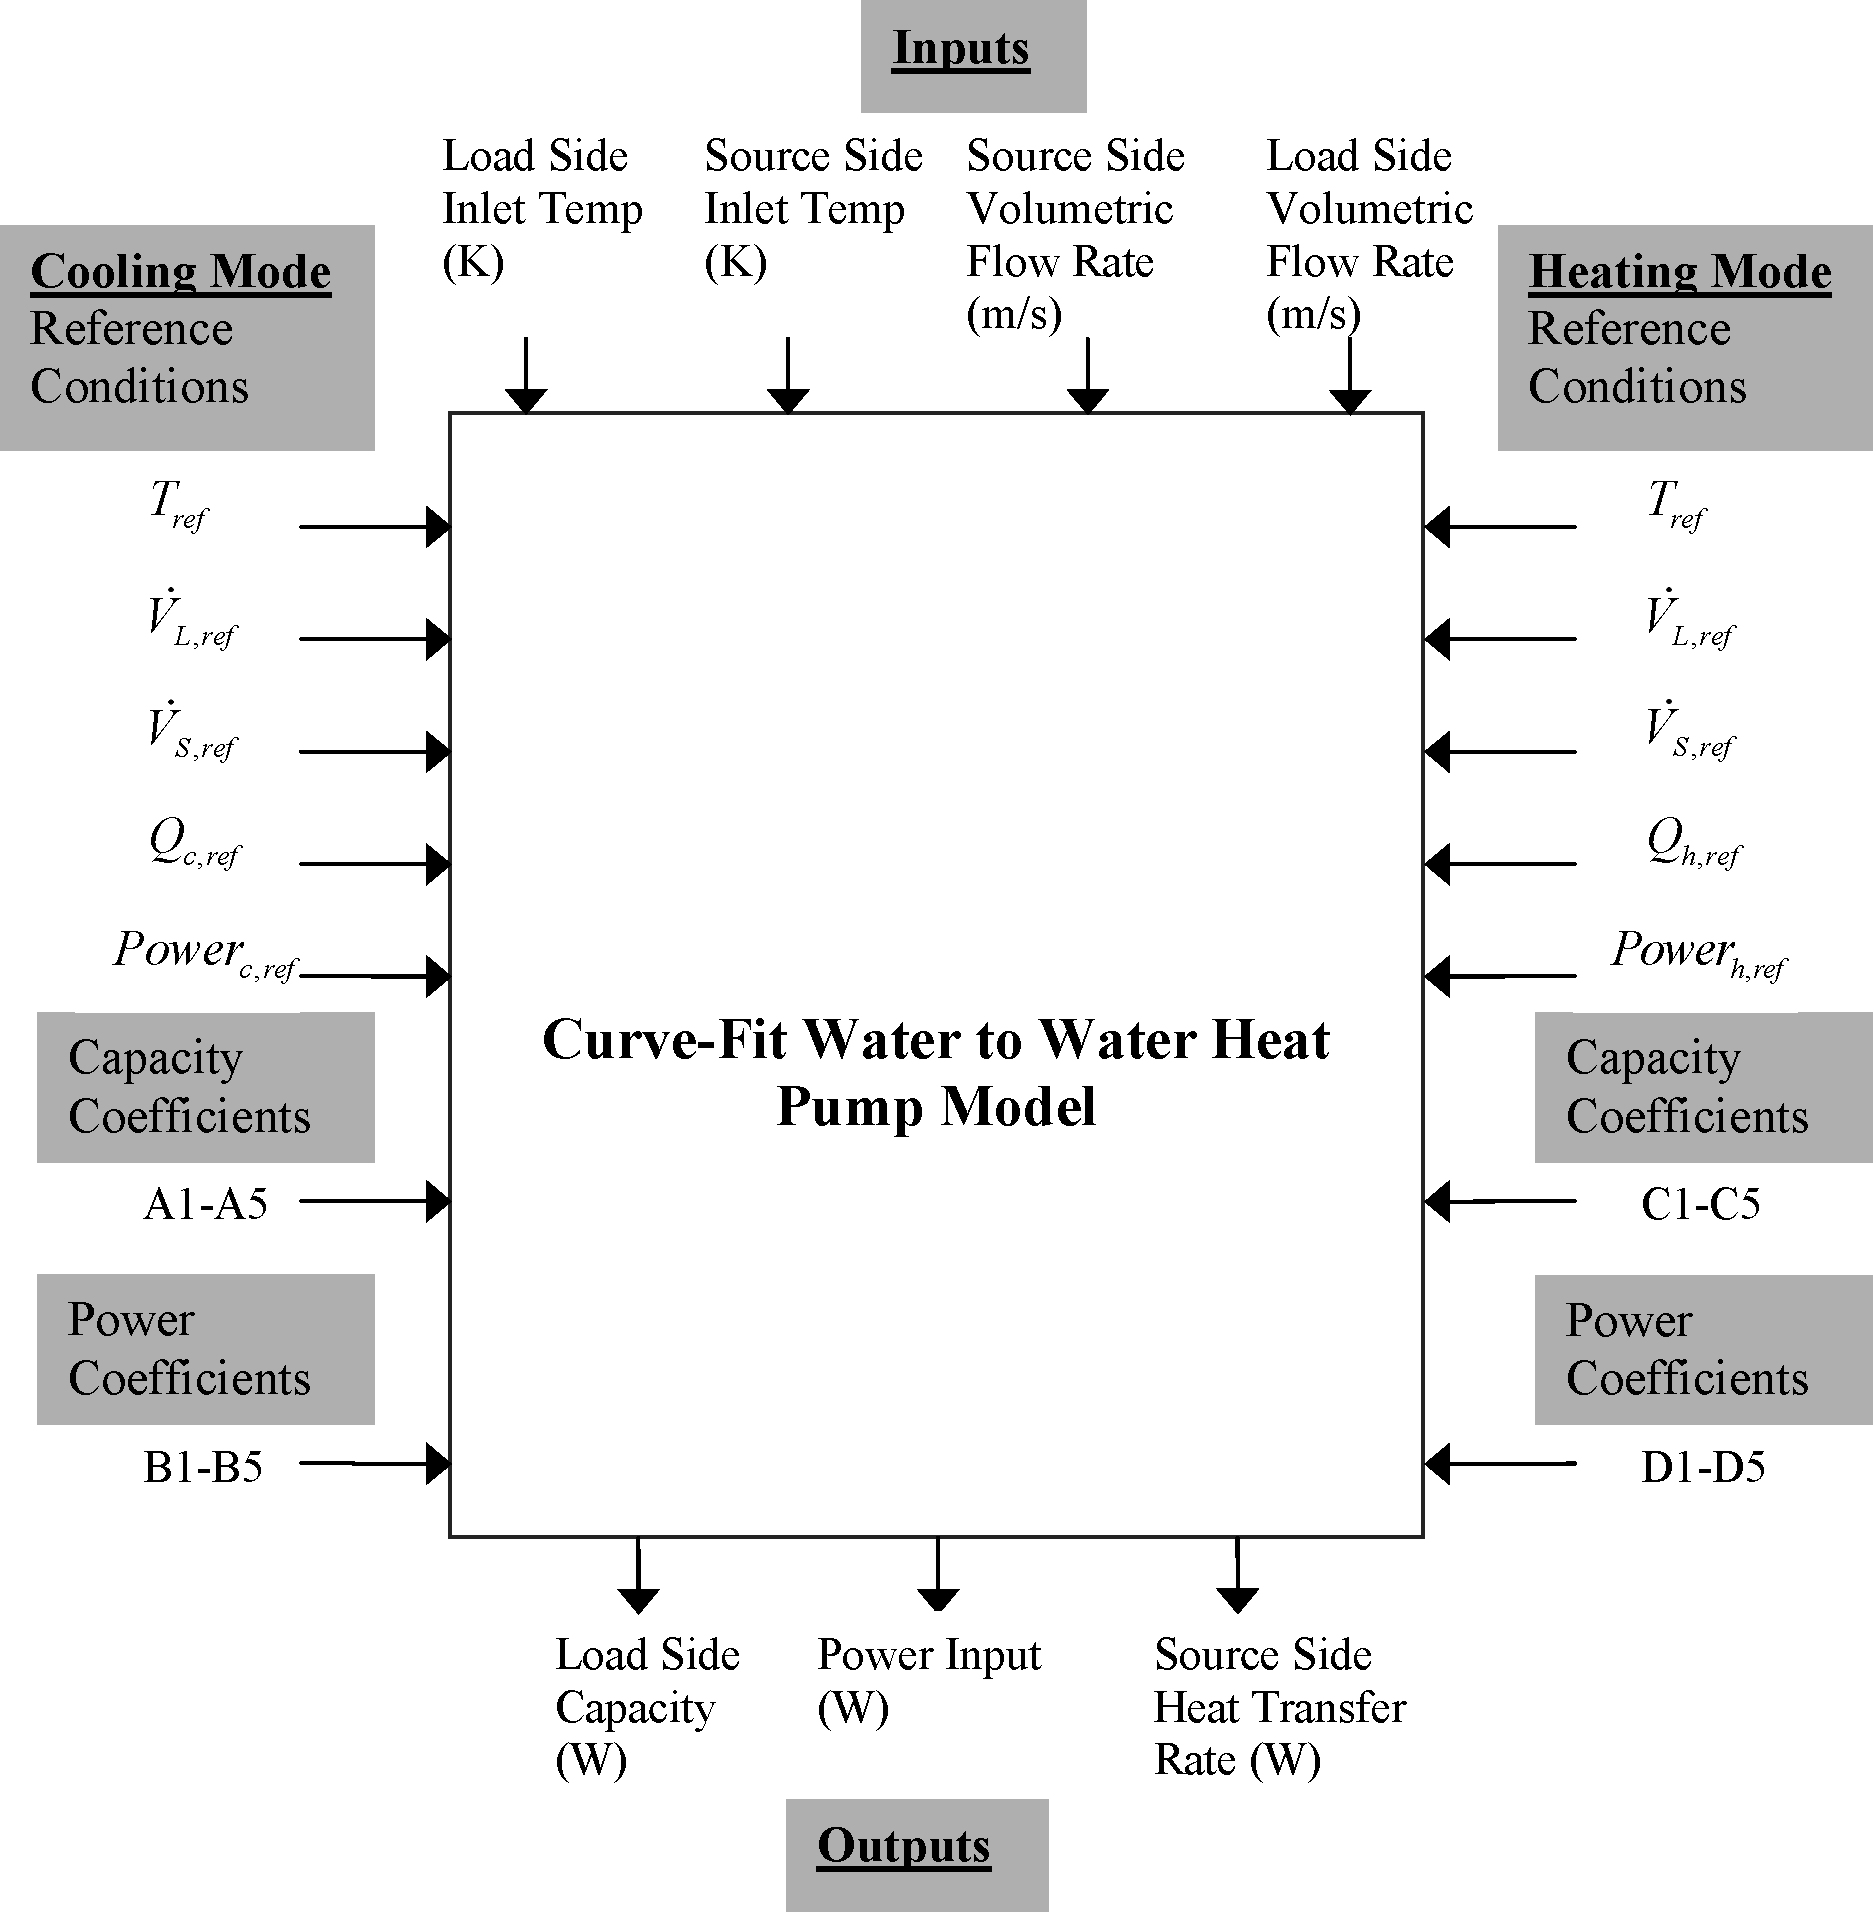
\includegraphics[width=0.9\textwidth, height=0.9\textheight, keepaspectratio=true]{media/image5290.png}
\caption{Information Flow Chart for Water-To-Water Heat Pump Equation Fit (Tang 2005) \protect \label{fig:information-flow-chart-for-water-to-water}}
\end{figure}

\subsection{Parameter Estimation Water-To-Water Heat Pump Model}\label{parameter-estimation-water-to-water-heat-pump-model}

A steady state simulation model for a water-to-water reciprocating vapor compression heat pump (Object names: HeatPump:WaterToWater:ParameterEstimation:Cooling \& HeatPump:WaterToWater:ParameterEstimation:Heating) is described in this section. This documentation is derived from the Ph.D.~dissertation of Hui Jin which is available on the Oklahoma State University web site . The model incorporates a multivariable unconstrained optimization algorithm to estimate several unspecific parameters. The aim of the model is to describe the detailed physical geometry and operation of each component and replicate the performance of the actual unit in operation. Assuming the thermodynamic process in the expansion device and the pressure drop at the suction and discharge valves to be isenthalpic the heat balance equation is given by

\begin{equation}
{\dot Q_s} = \dot W + {\dot Q_{_L}}
\end{equation}

where:

\({\dot Q_s}\) is the source side heat transfer rate (W)

\({\dot Q_L}\) is the load side heat transfer rate (W)

\(\dot W\) is the compressor power input (W).

The compressor model is based on an isentropic process shown in Figure~\ref{fig:schematic-indicator-diagram-for-a} governed by:

\begin{equation}
{PV^{\gamma}} = Constant
\end{equation}

where P is pressure and V is specific volume.

\begin{figure}[hbtp] % fig 239
\centering
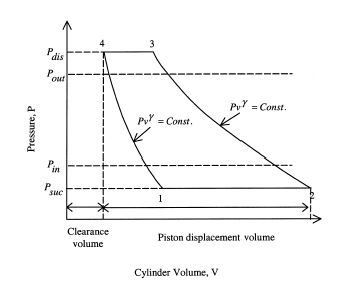
\includegraphics[width=0.9\textwidth, height=0.9\textheight, keepaspectratio=true]{media/image5296.png}
\caption{Schematic indicator diagram for a reciprocating Compressor(Jin 2002) \protect \label{fig:schematic-indicator-diagram-for-a}}
\end{figure}

Since the refrigerant vapor in the clearance volume as shown in the previous figure goes through a re-expansion procedure, the mass flow rate of the compressor refrigerant is a decreasing function of the pressure ratio.

\begin{equation}
{\dot{m}} = \frac{{PD}}{{\nu {}_{suc}}}\left( 1 + C - C{(\frac{{P{}_{dis}}}{{P{}_{suc}}})^{\frac{1}{\gamma }}} \right)
\end{equation}

where:

\({\dot{m}}\) is the refrigerant mass flow rate

PD is the piston displacement

C is the clearance factor

\(P_{dis}\) is the discharge pressure

\(P_{suc}\) is the suction pressure

\(\gamma\) is the isentropic exponent.

\subsubsection{Parameter estimation procedure}\label{parameter-estimation-procedure}

A set of parameters for the cooling mode is defined on the basis of the equations used in the model. An information flowchart indicating the parameters, inputs to the model and the resulting outputs acquired are shown in Figure~\ref{fig:information-flowchart-for-water-to-water-heat}. The estimation of parameters is conducted using the catalog data.

The parameter definition include:

\begin{itemize}
\item Piston displacement, PD
\item Clearance factor, C
\item Pressure drop across the suction and discharge valves, \({\rm{\Delta P}}\)
\item Loss factor used to define the electromechanical losses supposed to be proportional to the theoretical power, \({\rm{\eta }}\)
\item Superheat in \(^{\circ}\)C or F, \({\rm{\Delta T}}{}_{{\rm{sh}}}\)
\item Constant part of the electromechanical losses, \({\rm{W}}{}_{{\rm{loss}}}\)
\item Source side heat transfer coefficient, (UA)\(_{S}\)
\item Load side heat transfer coefficient, (UA)\(_{L}\)
\end{itemize}

\begin{figure}[hbtp] % fig 240
\centering
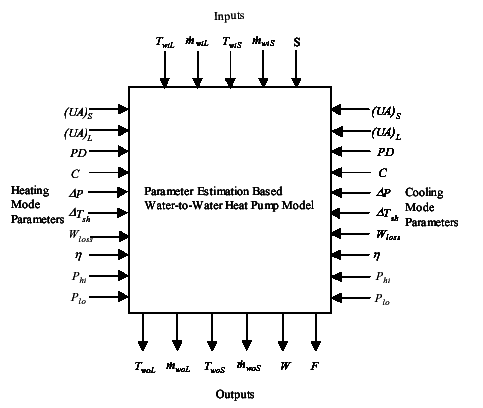
\includegraphics[width=0.9\textwidth, height=0.9\textheight, keepaspectratio=true]{media/image5306.png}
\caption{Information Flowchart for Water-To-Water Heat Pump Parameter Estimation Model implementation (Jin 2002) \protect \label{fig:information-flowchart-for-water-to-water-heat}}
\end{figure}

where:

TWiL is the entering water Load side temperature

TWiS is the entering water Source side temperature

\({\dot{m}_{WiL}}\) is the entering water Load side mass flow rate

\({\dot{m}_{WiS}}\) is the entering water Source side mass flow rate

S is the Thermostatic Signal.

The parameter estimation procedure incorporates an objective function that computes the difference between the model outputs and the catalog outputs.~ The objective function is then minimized by using a multi variable unconstrained multi modal Nelder Mead optimization algorithm. As the objective function value lowers after each iteration, the model outputs approach the catalog outputs consequently leading to convergence and the correct parameters are estimated for the respective model. The inputs to the model include the entering water temperatures and mass flow rates on the load side and the source side. The calculation of the objective function is shown in the form of a formula flowchart in Figure~\ref{fig:flow-diagram-of-energyplus-water-to-water}. The square of the sum of the errors (SSQE) for a given set of parameter values that will be minimized is given by:

\begin{equation}
SSQE = \sum\limits_{i = 1} {{{\left( {\frac{{\left( {\mathop {W{}_{cat}}\limits^{} } \right) - \left( {\mathop W\limits^{} } \right){}_i}}{{\left( {\mathop {W{}_{cat}}\limits^{} } \right)}}} \right)}^2}}  + \left( {\frac{{\left( {\mathop {QL{}_{cat}}\limits^{} } \right) - \left( {\mathop {QL}\limits^{} } \right){}_i}}{{\left( {\mathop {QL{}_{cat}}\limits^{} } \right)}}} \right)
\end{equation}

Where

\({\rm{W}}{}_{{\rm{cat}}}\) is the catalog power consumption

\({\rm{W}}{}_{}\) is the model power consumption

\({\rm{QL}}{}_{{\rm{cat}}}\) is the catalog load side heat transfer

\({\rm{QL}}{}_{}\) is the model load side heat transfer.

Extrapolation beyond the catalog data grants the parameter estimation model an upper hand in comparison with the equation fit and deterministic models. However, the detailed model is computationally more intensive. Moreover, when the model is implemented within a transient system simulation program, it may come across figures that are random and unplanned by the manufacturer such as low water flow rates or extreme temperatures. This oddity may result in unrealistic set of results.

\begin{figure}[hbtp] % fig 241
\centering
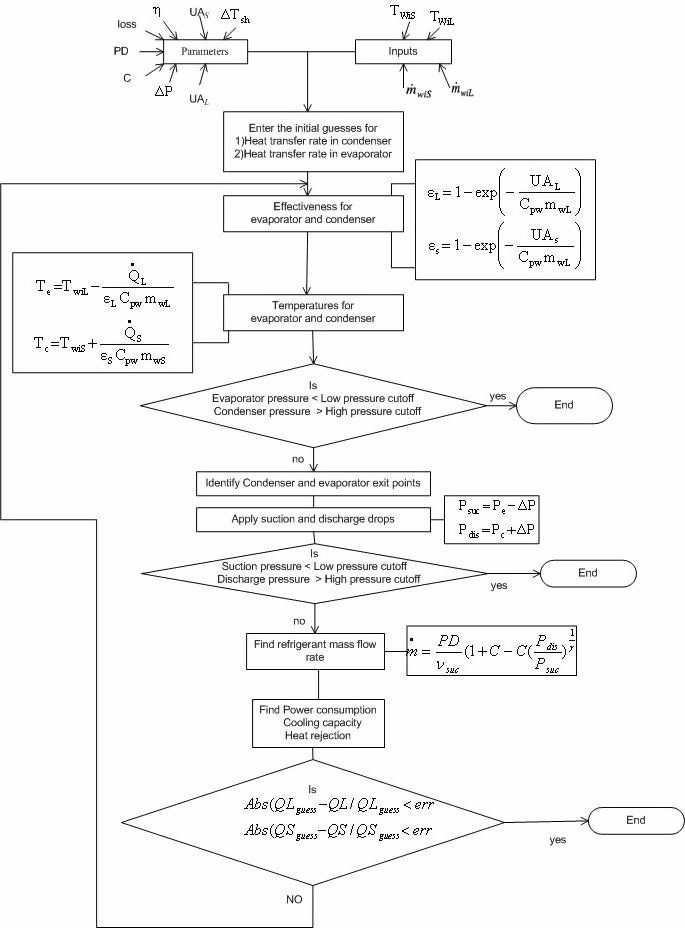
\includegraphics[width=0.9\textwidth, height=0.9\textheight, keepaspectratio=true]{media/image5314.png}
\caption{Flow diagram of EnergyPlus Water to Water Heat Pump implementation \protect \label{fig:flow-diagram-of-energyplus-water-to-water}}
\end{figure}

\subsubsection{Control Strategy}\label{control-strategy}

Both water-to-water heat pump models; parameter estimation based model and curve-fit model use the ``cycle time control logic'' developed by Murugappan (2002).

This strategy keeps the heat pump from short-cycling whereby the heat pump will stay on or off for the specified cycle time after switching states. The control logic is identical to the operation of a physical heat pump whereby the heat pump does not switch between on and off instantly. Refer to Muraggapan (2002) for the further details on the control strategy.

\subsubsection{References}\label{references-1}

Jin, Hui. 2002. Parameter Estimation Based Models of Water Source Heat Pumps. Phd. Thesis, Department of Mechanical and Aerospace Engineering, Oklahoma State University. (downloadable from \href{http://www.hvac.okstate.edu}{http://www.hvac.okstate.edu/})

Tang,C. C. 2005. Modeling Packaged Heat Pumps in Quasi-Steady State Energy Simulation Program. M.S. Thesis. Department of Mechanical and Aerospace Engineering, Oklahoma State University. (downloadable from \href{http://www.hvac.okstate.edu}{http://www.hvac.okstate.edu/})

Murugappan, Arun. 2002.~ Implementing Ground Source Heat Pump and Ground Loop Heat Exchanger Models in the EnergyPlus Simulation Environment, M.S. Thesis, Department of Mechanical and Aerospace Engineering, Oklahoma State University (downloadable from \href{http://www.hvac.okstate.edu}{http://www.hvac.okstate.edu/})

\subsection{EIR Formulated Plant Loop Heat Pump Model}\label{eir-plant-loop-heat-pump-model}

This section describes the EIR formulated model for plant loop heat pumps, which can be configured as either a water-source or air-source object. (Object names: HeatPump:PlantLoop:EIR:Cooling \& HeatPump:PlantLoop:EIR:Heating). The heating component has multiple defrost models to choose from and water outlet temperature minimum and maximum inputs to further control the unit, if desired. In general, these heat pump objects are treated the same as the other heat pump models by the plant loop.  Even though a heat pump is generally a single load coil and a single source coil with a reversing valve, in EnergyPlus, the paradigm is to split the operation into two separate coils, one for heating and another for cooling.  It is certainly possible to connect the load side of both of these to a single plant loop if the controls are established properly.  For water-source operation the source side of the coils are often placed on a single loop with some form of condensing supply, either a ground loop heat exchanger or a cooling tower (or a combination of the two). For air-source operation, the outdoor air node is used on the source-side inlet node. This is a typical congifiguration for chillers/boilers or heat pumps conditioning water loops that serve chilled or hot water coils.

For advanced plant configurations the heat pump could be connected to a cold and hot plant loop to move energy from one plant to another. This is a form of heat recovery that is used to meet small plant loads in one plant loop (e.g., heating) while the other plant loop is active (e.g., cooling). The activation of a heat recovery heat pump in this manner will reduce the active cooling plant load while meeting the heating plant load which improves the overall plant efficiency. In Energyplus the plants are separate and therefore the load side of one coil is connected to one loop (e.g., cooling) while the source side is connected to the other loop (e.g., heating). The corresponding coil would be connect in the opposite fashion where the load side is connected to the other loop (e.g., heating) while the source side is connected to the original loop (e.g., cooling). Given the constraints of a single mixer and splitter for a given plant loop this connection can be challenging. One possible connection option is to connect one coil's load side to the plant inlet branch while the source side is connected to the other plant's demand side outlet branch. Only 1 or the other coil is operating while the idle coil operates as a pass-through unit. The following figure shows the HeatPump:PlantLoop:EIR coils configured as typical air-cooled plant equipment on the supply side of each plant in parallel branches where a cooling and heating coil are considered a single heat pump (i.e., 2-pipe units AWHP-1, 2 and 3. These could also be 4-pipe units connected to a condenser or ground source loop.). Also shown is a 4-pipe water-to-water heat pump connected between the plant loops in a heat recovery configuration (as of V22.3). A heat pipe configured this way would required that both plant loops have flow and specialized controls to determine which coil operates (see PlantEquipmentOperation:ChillerHeaterChangeover). An important connection criteria for the 4-pipe heat recovery configuration is to connect the load side of the heat pump to the plant supply side inlet and the source side to the demand side outlet. The model will check whether there is a connection to the plant in this fashion and use that information to decide whether to add the heat pump water flow rates during plant sizing since this configuration should not increase plant design water flow rate.

\begin{figure}[hbtp]
\centering
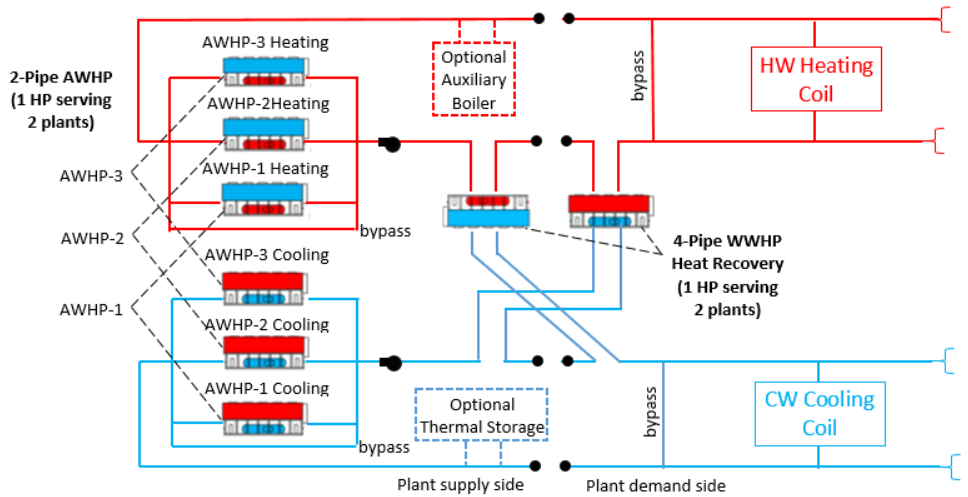
\includegraphics[width=0.9\textwidth, height=0.9\textheight, keepaspectratio=true]{media/ChillerHeaterPlantLoopEIRSchematic.png}
\caption{Schematic of the Cold and Hot water loops using Heat Pumps \protect \label{fig:schematic-of-the-energyplus-cold-and-hot-plant-loop-heat-pumps}}
\end{figure}

Note that this component is a constant or variable flow device (it will either request its full design flow from the plant or flow proportional to the operating part-load ratio). The heat pump can respond to a load or outlet node setpoint.

The bookkeeping part of the plant heat pump model with regards to flow requests and nodal conditions is similar to other water-to-water heat pump components. This section will briefly describe the mathematical formulation of the model and then itemize more detailed calculations.

Once load and source water flow rates have been established for the component, using the SetComponentFlowRate interface to the plant, and inlet temperatures for each side have been read, a model function calculates the response of the unit to these conditions. The process to evaluate the outlet state is as follows:

\begin{enumerate}
      \item Determine the operating water flow rate of the heat pump. Constant water flow heat pumps will operating at the design water flow rate and variable speed water flow heat pumps will operate at a water flow rate proportional to operating part-load ratio. In addition, if a heat pump is configured as a heat recovery unit (see figure) then the water flow rate is set as pass-through when the unit is off.
	\item If set point controlled, retrieve the load side temperature setpoint to determine the load on the heat pump. If load controlled, directly use the load passed to the model. 
	\item Evaluate the capacity modifier function using the load side setpoint temperature as the projected outlet temperature and the source inlet temperature ($CAPFT = f(T_{out,load,set}, T_{in,source}) $)
     \item Evaluate source outlet temperature limits and defrost operation, if selected, to determine the impact on operating capacity
	\item Calculate available load side capacity using the reference value and the modifier ($\dot{Q}_{avail} = \dot{Q}_{ref} \times CAPFT$)
	\item Calculate the part load ratio using the current plant-dispatched load (constrained between zero and one) ($PLR = \frac{\dot{Q}_{plant}}{\dot{Q}_{avail}}$)
	\item Calculate the actual operating load side heat transfer and the load side outlet temperature ($\dot{Q}_{load} = \dot{Q}_{avail}PLR$, $T_{out,load} = T_{in,load} \pm \frac{\dot{Q}_{load}}{\dot{m}_{load}C_{p,load}}) $) -- note the plus/minus refers to how the value will be added in heating mode and subtracted in cooling mode.
     \item Take the reference power usage as $P_{ref}$ = $Q_{ref}$ divided by $COP_{ref}$
	\item Evaluate power usage by evaluating the EIR curves using the target load side outlet temperature, source inlet temperature, and the current part load ratio ($EIRFT = f(T_{out,load,set}, T_{in,source})$, $EIRFPLR = f(PLR)$, $P = P_{ref} \times EIRFT \times EIRFPLR$)
	\item Perform an energy balance on the unit to determine the source side heat transfer rate and the source side outlet temperature ($\dot{Q}_{source} = \dot{Q}_{load} \pm P$, $T_{out,source} = T_{in,source} \pm \frac{\dot{Q}_{source}}{\dot{m}_{source}C_{p,source}} $) -- again the plus/minus refers to the different behavior between cooling and heating mode.
\end{enumerate}

The following sections identify model calculations in more detail:

\subsubsection{Water Flow Rate Initialization}\label{eir-air-to-water-heat-pumps-water-flow-rate-initialization}
The heat pump initially sets the load and source side water flow rates to either an off condition, a pass-through condition, or the design values to allow other plant components (e.g., pumps, boilers, coils, etc.) to operate if needed. If the plant is operating, the water flow rate is set according to logical progression from the initial iteration to the final iteration of a specific time step.

\begin{equation}
\dot{m}_{load} = \dot{m}_{rated}
\end{equation}
\begin{equation}
\dot{m}_{source} = \dot{m}_{source}
\end{equation}
On subsequent iterations, the flow rate is also set to the design values, however, if the pump is variable speed the load and source side water flow rates are set proportional to the operating part-load ratio from the previous iteration. When a load-side branch pump is used the load-side flow is also limited to the minimum pump flow rate. If the heat pump is air-cooled the source side flow is set to design without multiplying by operating part-load ratio. If the heat pump is off and is configured as a heat recovery heat pump connected to the supply side inlet and demand side outlet then the heat pump will allow the plant water to flow through the heat pump when the heat pump is off. For heat pumps that are connected to a parallel branch on the plant supply side (see figure for 2-pipe AWHPs) then the water flow rate is set to 0 when the heat pump is off.\\

When the heat pump is off and conncted to the plant supply side only:

\begin{equation}
\dot{m}_{load} = 0
\end{equation}
\begin{equation}
\dot{m}_{source} = 0\;\; (water-cooled\;only)
\end{equation}

When the heat pump is off and conncted to the plant supply side and plant demand side (heat recovery configuration):

\begin{equation}
\dot{m}_{load} = \dot{m}_{inlet,\;load}
\end{equation}
\begin{equation}
\dot{m}_{source} =  \dot{m}_{inlet,\;source}\;\; (water-cooled\;only)
\end{equation}

When the heat pump is on, regardless where the heat pump is connected, and the water flow rate is selected as constant flow:

\begin{equation}
\dot{m}_{load} = \dot{m}_{load,\; rated}
\end{equation}
\begin{equation}
\dot{m}_{source} = \dot{m}_{source,\; rated}\;\; (water-cooled\;only)
\end{equation}

When the heat pump is on, regardless where the heat pump is connected, and the water flow rate is selected as variable flow:

\begin{equation}
\dot{m}_{load} = \dot{m}_{load,\; rated} \times PLR_{operating},\;{(PLR_{min} \le PLR_{operating} \le 1)}\;\; (\dot{m} \ge VS_{branchpump,\; minflow})
\end{equation}
\begin{equation}
\dot{m}_{source} = \dot{m}_{source,\; rated} \times PLR_{operating},\;{(PLR_{min} \le PLR_{operating} \le 1)}\;\; (water-cooled\;only)
\end{equation}

\subsubsection{Operating Set Point}\label{eir-air-to-water-heat-pumps-operating-set-point}
If the plant loop operating scheme is set point based the loop set point is used. For component based controls the component outlet set point is used otherwise the plant loop set point is used. For dual set point control the lower set point is used for cooling and the higher set point is used for heating. In the following equations the operating set point temperature is $T_{setpoint}$.

\subsubsection{Heat Pump Performance Calculations}\label{eir-air-to-water-heat-pumps-heat-pump-performance-calculations}
Calculations begin by determing the operating capacity of the heat pump. The capacity of the heat pump is a function of the load-side outlet temperature and the source-side inlet temperature. The heat pump is assumed to meet the load-side temperature set point and therefore the load-side outlet temperature is assumed to be the set point temperature.
\begin{equation}
CAPFT = f(T_{setpoint}, T_{source,\; inlet})
\end{equation}
\begin{equation}
\dot{Q}_{avail} = \dot{Q}_{ref} \times CAPFT
\end{equation}

\subsubsection{Dry Outdoor Coil Calculations (Heating mode only)}\label{eir-air-to-water-heat-pumps-dry-coil-calculations}
For air-cooled heat pumps a dry coil correction factor, if used, is applied for heating operation. As the moisture content of the ambient air changes the heating capacity also changes. This change in performance is limited to an ambient relative humidity range of 60 - 90\% where below 60\% the outdoor coil is dry and reduces heating capacity and above 90\% the coil is fully wet and yields full heating capacity. In the following equations, below 60\% relative humidity the $Factor_{correction} = Factor_{correction,\;dry}$ and above 90\% relative humidity the $Factor_{correction} = 1$. These calculations apply only to heating operation.
\begin{equation}
RH_{range} = 90 - 60
\end{equation}
\begin{equation}
Factor_{correction,\;dry} = f(T_{ambient})
\end{equation}
\begin{equation}
%Real64 semiDryFactor = dryCorrectionFactor + (1.0 - dryCorrectionFactor) * ((RH90 - state.dataEnvrn->OutRelHum) / rangeRH);
Factor_{correction} = Factor_{correction,\;dry} + (1 - Factor_{correction,\;dry}) \times (1 - \frac{90 - RH_{ambient}}{RH_{range}})
\end{equation}
\begin{equation}
\dot{Q}_{avail} = \dot{Q}_{avail} \times Factor_{correction}
\end{equation}
\begin{equation}
PLR = \frac{\dot{Q}_{load}}{\dot{Q}_{avail}}
\end{equation}
\begin{equation}
T_{setpoint,\;min} = f(T_{ambient})
\end{equation}
\begin{equation}
T_{setpoint,\;max} = f(T_{ambient})
\end{equation}
\begin{equation}
T_{setpoint} = T_{setpoint,\;min} \le T_{setpoint} \le T_{setpoint,\;max}
\end{equation}
Since the capacity as a function of temperature (CAPFT) relies on $T_{setpoint}$ the above performance calculations are repeated. If the Minimum/Maximum Supply Water Temperature Curves are not used or the water temp limits are not exceeded then the calculations proceed without repeating.

\subsubsection{Part Load Ratio Calculations}\label{eir-air-to-water-heat-pumps-part-load-ratio-calculations}
The heat pump operates to meet a load or temperature set point and therefore will operate at less than full capacity for most operating hours. The heat pump will run the entire time step to the point where the part-load ratio (PLR) is below the minimum part-load ratio provided by the user. Below this point the heat pump will cycle on and off to meet the load.
\begin{equation}
CyclingRatio = 1
\end{equation}
\begin{equation}
PLR_{operating} = PLR
\end{equation}
\begin{equation}
CyclingRatio = \frac{PLR_{operating}}{PLR_{min}}, {(PLR_{operating}\le PLR_{min})}
\end{equation}
\begin{equation}
PLR = PLR_{min}, {(PLR_{operating}\le PLR_{min})}
\end{equation}
\begin{equation}
PLR_{operating} = PLR \times CyclingRatio, {(PLR_{operating}\le PLR_{min})}
\end{equation}


\subsubsection{Defrost Model Description (Heating mode only)}\label{eir-air-to-water-heat-pumps-defrost-model-description}
The plant heat pump as 3 Heat Pump Defrost Control types which will impact heat pump heating capacity. The valid choices are None, Timed, OnDemand or TimedEmpirical. When None is selected these calculations are not performed and defrost operation will not impact energy use. Otherwise, one of the following calculation sets are executed if the outdoor ambient temperature is less than or equal to the user entered Maximum Outdoor Dry Bulb Temperature For Defrost Operation. The defrost model reports are set to 0 when defrost is not used or not active. These calculations apply only to heating operation.

%                this->loadDueToDefrost = 0.0;
%                this->defrostEnergyRate = 0.0;
%                this->fractionalDefrostTime = 0.0;
\begin{equation}
\dot{Q}_{load,\; defrost} = {0}
\end{equation}
\begin{equation}
\dot{Q}_{defrost} = {0}
\end{equation}
\begin{equation}
Fraction_{defrost, time} = {0}
\end{equation}
When defrost is active the following calculations are performed according to the user selected defrost model:

\begin{equation}
% Real64 OutdoorCoilT = 0.82 * state.dataEnvrn->OutDryBulbTemp - 8.589;
T_{defrost, coil} = {0.82 \times T_{ambient} - 8.589}
\end{equation}
\begin{equation}
% Real64 OutdoorCoildw = max(1.0e-6, (state.dataEnvrn->OutHumRat - Psychrometrics::PsyWFnTdpPb(state, OutdoorCoilT, state.dataEnvrn->OutBaroPress)));
{w_{defrost, coil} = w_{ambient} - w_{sat}}, where\; {w_{sat} = f(T_{dewpoint},\; Pressure_{ambient})}
\end{equation}

\subsubsection*{Timed Defrost Model:}\label{eir-air-to-water-heat-pumps-timed-defrost}

%                this->fractionalDefrostTime = this->defrostTime; // DefrostTime in hours
%                HeatingCapacityMultiplier = 0.909 - 107.33 * OutdoorCoildw;
%                InputPowerMultiplier = 0.90 - 36.45 * OutdoorCoildw;
%                this->loadDueToDefrost =
%                    (0.01 * this->fractionalDefrostTime) * (7.222 - state.dataEnvrn->OutDryBulbTemp) * (this->referenceCapacity / 1.01667);
%                Real64 defrostEIRFT = 1.0 / this->referenceCOP;
%                if (defrostEIRFTIndex > 0) {
%                    defrostEIRFT = Curve::CurveValue(
%                        state, this->defrostEIRFTIndex, max(15.555, state.dataEnvrn->OutWetBulbTemp), max(15.555, state.dataEnvrn->OutDryBulbTemp));
%                }
%                this->defrostEnergyRate = defrostEIRFT * (this->referenceCapacity / 1.01667) * this->fractionalDefrostTime;
\begin{equation}
Fraction_{defrost, time} = user\; input,\; Heat\; Pump\; Defrost\; Time\; Period\; Fraction
\end{equation}
\begin{equation}
Multiplier_{heating,\; capacity} = {0.909 - 107.33 \times w_{defrost,\; coil}}
\end{equation}
\begin{equation}
Multipler_{heating,\; power} = {0.90 - 36.45 \times w_{defrost,\; coil}}
\end{equation}
\begin{equation}
\dot{Q}_{load,\; defrost} = {0.01 \times Fraction_{defrost,\; time} \times (7.222 - T_{ambient}) \times (\frac{Q_{ref}}{1.01667})}
\end{equation}
\begin{equation}
EIRFT_{defrost} = \frac{1}{COP_{ref}}
\end{equation}
If the Defrost Energy Input Ratio Function of Temperature Curve has been entered by the user this curve will update the value of $EIRFT_{defrost}$. This performance curve is a function of outdoor wet-bulb temperature and outdoor dry-bulb temperature. If either of these outdoor temperatures are below 15.555 C, the minimum temperature of 15.555 C is used.
\begin{equation}
{EIRFT_{defrost} = f(T_{ambient,\; wetbulb}, T_{ambient})}
\end{equation}
\begin{equation}
\dot{Q}_{defrost} = EIRFT_{defrost} \times \frac{Q_{ref}}{1.01667} \times Fraction_{defrost,\; time}
\end{equation}

\subsubsection*{On Demand Defrost Model:}\label{eir-air-to-water-heat-pumps-on-demand-defrost}
%            this->fractionalDefrostTime = 1.0 / (1.0 + 0.01446 / OutdoorCoildw);
%            HeatingCapacityMultiplier = 0.875 * (1.0 - this->fractionalDefrostTime);
%            InputPowerMultiplier = 0.954 * (1.0 - this->fractionalDefrostTime);
%            this->loadDueToDefrost =
%                (0.01 * this->fractionalDefrostTime) * (7.222 - state.dataEnvrn->OutDryBulbTemp) * (this->referenceCapacity / 1.01667);
%            Real64 defrostEIRFT = 0.0;
%            if (defrostEIRFTIndex > 0) {
%                defrostEIRFT = Curve::CurveValue(
%                    state, this->defrostEIRFTIndex, max(15.555, state.dataEnvrn->OutWetBulbTemp), max(15.555, state.dataEnvrn->OutDryBulbTemp));
%            }
%            this->defrostEnergyRate = defrostEIRFT * (this->referenceCapacity / 1.01667) * this->fractionalDefrostTime;
\begin{equation}
Fraction_{defrost, time} = \frac{1}{1+\frac{0.01446}{w_{defrost,\; coil}}}
\end{equation}
\begin{equation}
Multiplier_{heating,\; capacity} = {0.875 \times Fraction_{defrost,\; time}}
\end{equation}
\begin{equation}
Multipler_{heating,\; power} = {0.954 \times (1 - Fraction_{defrost,\; time})}
\end{equation}
\begin{equation}
\dot{Q}_{load,\; defrost} = {0.01 \times Fraction_{defrost,\; time} \times (7.222 - T_{ambient}) \times (\frac{\dot{Q}_{ref}}{1.01667})}
\end{equation}
\begin{equation}
EIRFT_{defrost} = 0
\end{equation}
If the Defrost Energy Input Ratio Function of Temperature Curve has been entered by the user this curve will update $EIRFT_{defrost}$.  If either of these outdoor temperatures are below 15.555 C, the minimum temperature of 15.555 C is used.
\begin{equation}
{EIRFT_{defrost} = f(T_{ambient,\; wetbulb}, T_{ambient})}
\end{equation}
\begin{equation}
\dot{Q}_{defrost} = EIRFT_{defrost} \times \frac{\dot{Q}_{ref}}{1.01667} \times Fraction_{defrost,\; time}
\end{equation}

\subsubsection*{Timed Empirical Defrost Model:}\label{eir-air-to-water-heat-pumps-timed-empirical-defrost}
%            // cycles of defrost per hour
%            Real64 thisHourDefrostCycles = Curve::CurveValue(state, this->defrostFreqCurveIndex, state.dataEnvrn->OutDryBulbTemp);
%            // is directly proportional to the ratio of capacity used for that hour (PLR)
%            thisHourDefrostCycles *= operatingPLR;
%            // fraction of heat load per cycle of defrost
%            Real64 thisHourDefrostHeatLoad = 0.0;
%            if (this->defrostLoadCurveDims == 2) { // BiQuadratic
%                thisHourDefrostHeatLoad =
%                    Curve::CurveValue(state, this->defrostHeatLoadCurveIndex, state.dataEnvrn->OutWetBulbTemp, state.dataEnvrn->OutDryBulbTemp);
%            } else {
%                thisHourDefrostHeatLoad = Curve::CurveValue(state, this->defrostHeatLoadCurveIndex, state.dataEnvrn->OutDryBulbTemp);
%            }
%            // heat load is applied to full load (not rated) and is proportional to defrost cycles per hour
%            this->loadDueToDefrost = availableCapacity * thisHourDefrostHeatLoad * thisHourDefrostCycles;
%            // electric input fraction due to defrost
%            Real64 defrostHeatEnergyFraction = 0.0;
%            if (this->defrostEnergyCurveDims == 2) { // BiQuadratic
%                defrostHeatEnergyFraction =
%                    Curve::CurveValue(state, this->defrostHeatEnergyCurveIndex, state.dataEnvrn->OutWetBulbTemp, state.dataEnvrn->OutDryBulbTemp);
%            } else {
%                defrostHeatEnergyFraction = Curve::CurveValue(state, this->defrostHeatEnergyCurveIndex, state.dataEnvrn->OutDryBulbTemp);
%            }
%            // defrost energy rate is applied to rated power and is proportional to defrost cycles per hour
%            this->defrostEnergyRate = (this->referenceCapacity / this->referenceCOP) * defrostHeatEnergyFraction * thisHourDefrostCycles;
%
%            // question on how these multipliers are accounted for with capacity and power (e.g., 1+ or 1-)
%            InputPowerMultiplier = 1.0 + thisHourDefrostHeatLoad;
%            HeatingCapacityMultiplier = 1.0 + (thisHourDefrostHeatLoad * thisHourDefrostCycles);
%            this->fractionalDefrostTime = thisHourDefrostCycles * this->fractionalDefrostTime;
The model for Timed Empirical Defrost uses a Timed Empirical Defrost Frequency Curve to determine the number of defrost cycles that occur each hour. The number of defrost cycles is multiplied by the operating part-load ratio to determine the defrost cycle frequency. The heat load due to defrost is also initialized to 0.
\begin{equation}
{Cycles_{defrost} = f(T_{ambient})} \times PLR_{operating}
\end{equation}
\begin{equation}
Heat_{load,\; defrost} = 0
\end{equation}
The heat load per cycle of defrost is calculated based on a user provided performance curve. This curve can be either a univariate or bivariate using one of the following equations. If the Timed Empirical Defrost Heat Load Penalty Curve has been entered by the user this curve will update $Heat_{load,\; defrost}$ as:
\begin{equation}
Heat_{load,\; defrost} = f(T_{ambient})
\end{equation}
\begin{equation}
Heat_{load,\; defrost} = f(T_{ambient,\;wetbulb})
\end{equation}
The heat load per cycle of defrost is applied to the available capacity and is proportional to the defrost cycle per hour as: 
\begin{equation}
\dot{Q}_{defrost} = \dot{Q}_{avail} \times Heat_{load,\; defrost} \times Cycles_{defrost}
\end{equation}
\begin{equation}
Fraction_{heat,\; energy} = 0
\end{equation}
The defrost input energy fraction is calculated based on a user provided performance curve. This curve can be either a univariate or bivariate using one of the following equations. If the Timed Empirical Defrost Heat Input Energy Fraction Curve has been entered by the user this curve will update $Fraction_{heat,\; energy}$ as:
\begin{equation}
Fraction_{heat,\; energy} = f(T_{ambient})
\end{equation}
\begin{equation}
Fraction_{heat,\; energy} = f(T_{ambient,\;wetbulb},\;T_{ambient})
\end{equation}
\begin{equation}
DefrostPower = \frac{\dot{Q}_{ref}}{COP_{ref}} \times Fraction_{heat,\; energy} \times Cycles_{defrost}
\end{equation}
\begin{equation}
Multiplier_{heating,\; capacity} = {1 + (Heat_{load,\; defrost} \times Cycles_{defrost})}
\end{equation}
\begin{equation}
Multipler_{heating,\; power} = {(1 + Heat_{load,\; defrost})}
\end{equation}
\begin{equation}
Fraction_{defrost, time} = user\; input, Heat\; Pump\; Defrost\; Time\; Period\; Fraction \times Cycles_{defrost}
\end{equation}

These defrost method calculations, if used, will result in an adjustment to the available heating capacity as:

\begin{equation}
\dot{Q}_{avail} *= Multiplier_{heating,\; capacity};
\end{equation}

\subsubsection{Final Calculation of Load and Energy, Power and Electricity, and Outlet Conditions}\label{eir-air-to-water-heat-pumps-final-calculations}
The plus/minus in a few of the following equations differentiates behavior between cooling and heating.
\begin{equation}
\dot{Q}_{load} = \dot{Q}_{avail} \times PLR_{operating}
\end{equation}
\begin{equation}
{Q}_{load} = \dot{Q}_{load} \times TimeStepInSeconds
\end{equation}
\begin{equation}
T{out,\;load} = T_{in,\;load} \pm \frac{\dot{Q}_{load}}{\dot{m}_{load}} \times C_{p,\;load}
\end{equation}
\begin{equation}
EIRFT = {f(T_{out,\;load}, T_{in,\;source})}
\end{equation}
\begin{equation}
EIRFPLR = {f(PLR_{operating})}
\end{equation}
\begin{equation}
Power = \frac{\dot{Q}_{load}}{COP_{ref}} \times EIRFT \times EIRFPLR \times Multipler_{heating,\; power} \times CyclingRatio
\end{equation}
\begin{equation}
Energy = Power \times TimeStepInSeconds
\end{equation}
\begin{equation}
{\dot{Q}_{source} = (\dot{Q}_{load} \pm Power) \times CyclingRatio}
\end{equation}
\begin{equation}
T{out,\;source} = T_{in,\;source} \pm \frac{\dot{Q}_{source}}{\dot{m}_{source} \times C_{p,\;source}}
\end{equation}
\begin{equation}
{Q}_{source} = \dot{Q}_{source} \times TimeStepInSeconds
\end{equation}

\subsection{Fuel-Fired Air to Water Heat Pumps}\label{fuel-fired-air-to-water-heat-pumps}

This section describes the EIR formulated model for fuel-fired plant loop absorption air-to-water heat pumps. The object is similar to a conventional air-to-water heat pump, except that it uses an absorption cycle driven by fuel combustion. The object names are HeatPump:AirToWater:FuelFired:Heating and HeatPump:AirToWater:FuelFired:Cooling. In general, these heat pump objects are treated in the same way as the other plant loop heat pump models. When dealing with the heating and cooling modules of the equipment, it uses a similar paradigm as the electric-driven \hyperref[eir-plant-loop-heat-pump-model]{EIR Formulated Plant Loop Heat Pump}: even though a heat pump is generally a single load coil and a single source coil with a reversing valve, in EnergyPlus, the paradigm is to split the operation into two separate units, one for heating a hot water loop and one for cooling a chilled water loop. It is certainly possible to connect the load side of both of these to a single plant loop if the controls are established properly. This equipment only supports air-source operation with an outdoor air node used as the source-side inlet node.

The underlying fuel-fired absorption heat pump model uses equation-fit models based on manufacturer data. The implemented model is as follows: 

\subsubsection{Equipment Capacity}
The heating and cooling capacities are derived from the nominal (rated) capacity and a capacity function of temperatures. 
\begin{equation}
\mathrm{GAHP Heating/Cooling Capacity} = \mathrm{Rated Capacity} \times \mathrm{CAPFT}
\end{equation}

The temperatures used for the equation model are the ambient air temperature ($T_{mathrm{amb}}$) and the returning (or entering) water temperature ($T_{\mathrm{ret}}$) of the load side.
\begin{equation}
\mathrm{CAPFT} = a_1 \times T_{\mathrm{amb}} + b_1 \times T_{\mathrm{amb}}^{2} + c_1 \times T_{\mathrm{ret}} + d_1 \times T_{\mathrm{ret}}^{2} + e_1 \times T_{\mathrm{amb}} \times T_{\mathrm{ret}} + f_1
\end{equation}

\subsubsection{Part Load Ratio}
Part Load Ratio is the ratio for the actual heating/cooling load over the current full capacity load. In real absorption machines, the PLR is usually between 0.2 and 1.0. 
\begin{equation}
\mathrm{PLR} = \frac{\mathrm{Load}}{\mathrm{Capacity}}, 0.2 \leq \mathrm{PLR} \leq 1
\end{equation}

\subsubsection{Fuel Use}
The fuel usage is calculated using the following formula, taking consideration of the load capacity, nominal COP, and the various adjustment factors (temperature, PLR, Defrosting, and Cycling Ratio):

\begin{equation}
\mathrm{Fuel Use} = \frac{\mathrm{Load} \times \mathrm{EIRFT} \times \mathrm{EIRFPLR} \times \mathrm{EIRDEFROST}}{\mathrm{COP}_\mathrm{nominal} \times \mathrm{CRF}}
\end{equation}

\subsubsection{EIR Temperature Adjustment}
A typical EIR temperature correction function will involve two independent temperature variables---the ambient air temperature ($T_{mathrm{amb}}$) and the returning (or entering) water temperature ($T_{\mathrm{ret}}$) of the load side. 
\begin{equation}
\mathrm{EIRFT} = a_2 \times Tamb + b_2 \times T_{\mathrm{amb}}^{2} + c_2 \times T_{\mathrm{ret}}^{2} + d_2 \times T_{\mathrm{ret}}^{2} + e_2 \times T_{\mathrm{amb}} \times T_{\mathrm{ret}} + f_2
\end{equation}

\subsubsection{EIR PLR Adjustment}
The EIR PLR correction function is a cubic function that takes the PLR as the sole independent variable. For example, a potential curve can be used is like the following:  
\begin{equation}
\mathrm{EIRFPLR} = 0.0865 \times \mathrm{PLR}^{2} - 0.006 \times \mathrm{PLR} + 0.9814, \mathrm{for} 0.25 \leq \mathrm{PLR} \leq 1 
\end{equation}

\subsubsection{Defrosting Adjustment (Heating mode only)}
If the defrost control type is OnDemand, then the defrost fuel use correction is modeled using the ambient air temperature as the independent variable. The inputs allows a cubic (or lower order) function. For example, one possible curve correlation can look like the following:  
\begin{equation}
\mathrm{EIRDEFROST} = -0.0011 \times T_{\mathrm{amb}}^{2} - 0.006 \times T_{\mathrm{amb}} + 1.0317, \mathrm{for} -8.89^{\circ}\mathrm{C} \leq T_{\mathrm{amb}} \leq 3.33^{\circ}\mathrm{C} 
\end{equation}

\subsubsection{Cycling Ratio Adjustment}
The cycling ratio correction is also used for fuel use calculations when the PLR is below the minimum. This curve can be inputted by the user. An example correlation for CRF is as follows: 
\begin{equation}
\mathrm{CRF} = 0.4167 \times \mathrm{CR} + 0.5833,
\end{equation}

where $\mathrm{CRF}$ is the Cycling Ratio Factor; and $\mathrm{CR}$ is the Cycling Ratio, which is defined as: 

\begin{equation}
\mathrm{CR} = \frac{\mathrm{PLR}}{\mathrm{PLR}_{\mathrm{min}}}, \mathrm{for} 0.2 \leq \mathrm{PLR} \leq 0.25
\end{equation}

Please note that since the object is based on curve inputs, the user also has the flexibility of defining the curves by themselves---e.g. from the capacity function of temperature to the defrost EIR corrections. 

\subsubsection{Electricty Use}

The electricity use for the fuel-fired absorption heat pump is modeled using EIR (Electricity based relation) input curves. The two part of electricity use is the ``auxiliary electricity'' and the ``standby electricity'':
\begin{equation}
\mathrm{Electricity use} = \mathrm{Norminal Auxiliary Power} \times \mathrm{EIR}_{\mathrm{auxiliary}} + \mathrm{Electricty}_{\mathrm{Standby}},
\end{equation}
where $\mathrm{EIR}_{\mathrm{auxiliary}}$ are supplied by the curve input, and $\mathrm{Norminal Auxiliary Power}$ and $\mathrm{Electricty}_{\mathrm{Standby}}$ are supplied by the equipment standby electricity inputs. 
